\section{Йерархия на сигмоидните модели}
\subsection{Експериментът на Марков и Стойчева}
Тук ще прехвърлим фокуса от получаването на конкретен модел към изграждане на кратка йерархия на база поведение, брой параметри, физичен смисъл на параметрите и т.н. Експерименталните данни, спрямо които ще сравняваме моделите са тези на \textit{Марков и Стойчева} от 1976~г. \cite{Markov1976}. Това са едни от най-фините експерименти за зародишообразуване под действието на външен електричен потенциал.

В този експеримент е изследван броят на зародишите като функция на времето и  концентрацията на електролит при електроотлагане на $Hg$ от воден разтвор на $Hg_2(NO_3)_2$ върху ,,безсктруктурен`` \textit{планарен} $Pt$-електрод. В статията си \textit{Марков и Стойчева} правят заключение, че в началото има \textit{линейно нарастване} на броя зародиши и след това се достига плато. Броят зародиши, в платото зависи от експерименталните условия. От \textit{Фиг. 5} на \textit{Марков и Стойчева} се вижда, че броят зародиши всъщност следва сигмоиден закон. Още повече, отлагането върху планарен електрод предполага \textit{квази-двумерен растеж} $(D=2)$. Тези експериментални условия ще бъдат важни за избора на модел, като най-подходящ от разглежданите.

\subsection{Модели за описание на данните}
Ще използваме по-общата дефиниция на степен на превръщане \autoref{eq:alpha_ndef_def} през $N(t)$, тъй като експериментът е именно за броя образувани зародиши. Допълнително, максималният брой зародиши $N_{max}$, ще направим параметър на модела, подлежащ на идентификация. Общо трите модела, които ще разгледаме, ще записваме във вида:

\begin{equation*}
    N(t) = N_{max} f(\overline{p}, t)
\end{equation*}
Където $f(\overline{p}, t)$ е дясната страна на интегралната сигмоидна крива за конкретния модел, $t$ - време,  $\overline{p}$ e векторът с параметрите, освен $N_{max}$.
Трите модела, които ще разгледаме са Ричардс, JMAKn и $\alpha_{21}$.
\paragraph{Модел на Ричардс.} Това е един от най-общите модели на сигмоиден растеж, с множител отчитащ положителната обратна връзка и такъв, отчитащ самоограничаването поради изчерпване на ресурс (пресищането в контекста на кристалния растеж). Той е изведен като обобщение на логистичните модели в контекста на описание на растежа на популации. Диференциалната форма на Ричардс е:
\begin{equation}
    \label{eq:richards_diff_form}
    \frac{d(N/N_{max})}{dt} = \frac{k N}{N_{max}(q-1)}\left[ 1 - \left(\frac{N}{N_{max}}\right)^{q-1} \right]
\end{equation}
В основното ОДУ се вижда, че членът отговарящ за положителната обратна връзка води до $N \propto e^t$ за малки времена. Това ОДУ може да бъде интегрирано точно, за да бъде получено решение в затворен вид \cite{Richards1959}:
\begin{equation}
    \label{eq:richards_int_form}
    N(t) = \frac{N_{max}}{\left\{1 + (q-1)\exp{\left[ - (t-t_{i})/t_k \right]}\right\}^{\frac{1}{q-1}}}
\end{equation}
Където $t_k = 1/k$, е характеристичното време на процеса, $k$ - кинетичен коефициент, $t_{i}$ е времето, в което се достига инфлексната точка. Може да се покаже \cite{Tjrve2010}, че $N_i (t_i) = N_{max} d ^ {\frac{1}{1-d}}$. И съответно времевата скала е:
\begin{equation*}
    \tau_R = t_i q ^ {\frac{1}{q-1}}
\end{equation*}
Рескалираме и получаваме безразмерната форма:
\begin{equation*}
    \alpha \equiv \frac{N(t)}{N_{max}} = \left[ 1 + (q-1) \exp{\left( -K \left( \frac{t}{\tau_R} - q ^ {\frac{1}{1-q}} \right) \right)} \right] ^ {\frac{1}{1-q}}
\end{equation*}
Така в модела остават 2 параметъра (спрямо безразмерното време $t/\tau_R$): $K \coloneqq q^{1/(q-1)} t_i / t_k$ и $q$. Тогава и позицията на инфлексната точка е на линията $\alpha = t/\tau_R$ и не зависи от избора на $q$ и $K$.
Изборът на $q = 2$ дава познатият модел на Ферхюлст, a при $q = 1$ - Гомперц (граничен преход). Заедно с времевата скала, за
$\overline{p} = (q, K, \tau_R)$. Тогава за целите на параметричната идентификация имаме \textbf{четири} параметъра, които трябва да определим.

\paragraph{Модел JMAKn.} Ще използваме интегралната крива във вида даден от \autoref{eq:jmakn_with_time_scale}, като заместим степента на превръщане с $N$ през \autoref{eq:alpha_ndef_def}. Получаваме:
\begin{equation}
    \label{eq:jmakn_intform_n}
    N(t) = N_{max} \left\{ 1 - \exp{\left[  \left( 2 \frac{t}{\tau_{JMAK}} \right)^n \right]} \right\}
\end{equation}
Параметрите са степента $n$ (вж. \autoref{prem:jmak}) и времевата $\tau_{JMAK}$. Тогава $\overline{p} = (n, \tau_{JMAK})$. Заедно с $N_{max}$ параметрите за определяне в този случай са \textbf{три}.

\paragraph{Модел $\boldsymbol{\alpha_{21}}$.} Тъй като експерименталните условия предполагат квази-двумерен растеж, тук директно ще използваме вариацията на $\aDg$ с $D = 2$, $g = 1$. Предимствата на този модел спрямо JMAKn в близък експериментален контекст  бяха описани в \autoref{sub:experimental_validation}. Единствено остава да запишем кривата за $\alpha_{21}$ от \autoref{sub:analytic_results} като такава за $N(t)$:
\begin{equation}
    \label{eq:alpha21_intform_n}
    N(t) = N_{max} \tanh^2{\left( 2 \frac{t}{\tau_{21}} \right)}
\end{equation}
Тук $\overline{p} = (\tau_{21})$. Заедно с $N_{max}$ общият брой параметри подлежащи на определяне е \textbf{два}.

Моделите следват ясна йерархия в броя параметри, като най-много са при Ричардс и най-малко - при $\alpha_{21}$. Най-ценен ще е такъв модел, който може да даде най-добро физично описание с най-малък брой параметри. Т.е., ако $\alpha_{21}$ дава съизмерими по $R^2$ резултати на Ричардс, ние бихме предпочели $\alpha_{21}$ заради по-малкия брой параметри и заради по-ясния им смисъл в контекста на кристализация.

Тук няма да се ограничим само с определянето на скалите за всеки конкретен модел и набор данни от \textit{Фиг. 5 и 6} от \cite{Markov1976}, a ще разгледаме зависимостта параметрите на модела и най-вече времевите скали от свръхпотенциала, при който е проведена кристализацията (еквивалент на пресищане).

\subsection{Резултати от определянето на параметрите}
\subsubsection{Модел на Ричардс}
\begin{figure}[hbpt]
    \centering
    \caption{Рескалирани данни с параметрите получени за модела на Ричардс (вж. също \cite{VikiPHD2023} \cite{ivanmarkovpreprint})}
        \subfloat[Фиг. 5]{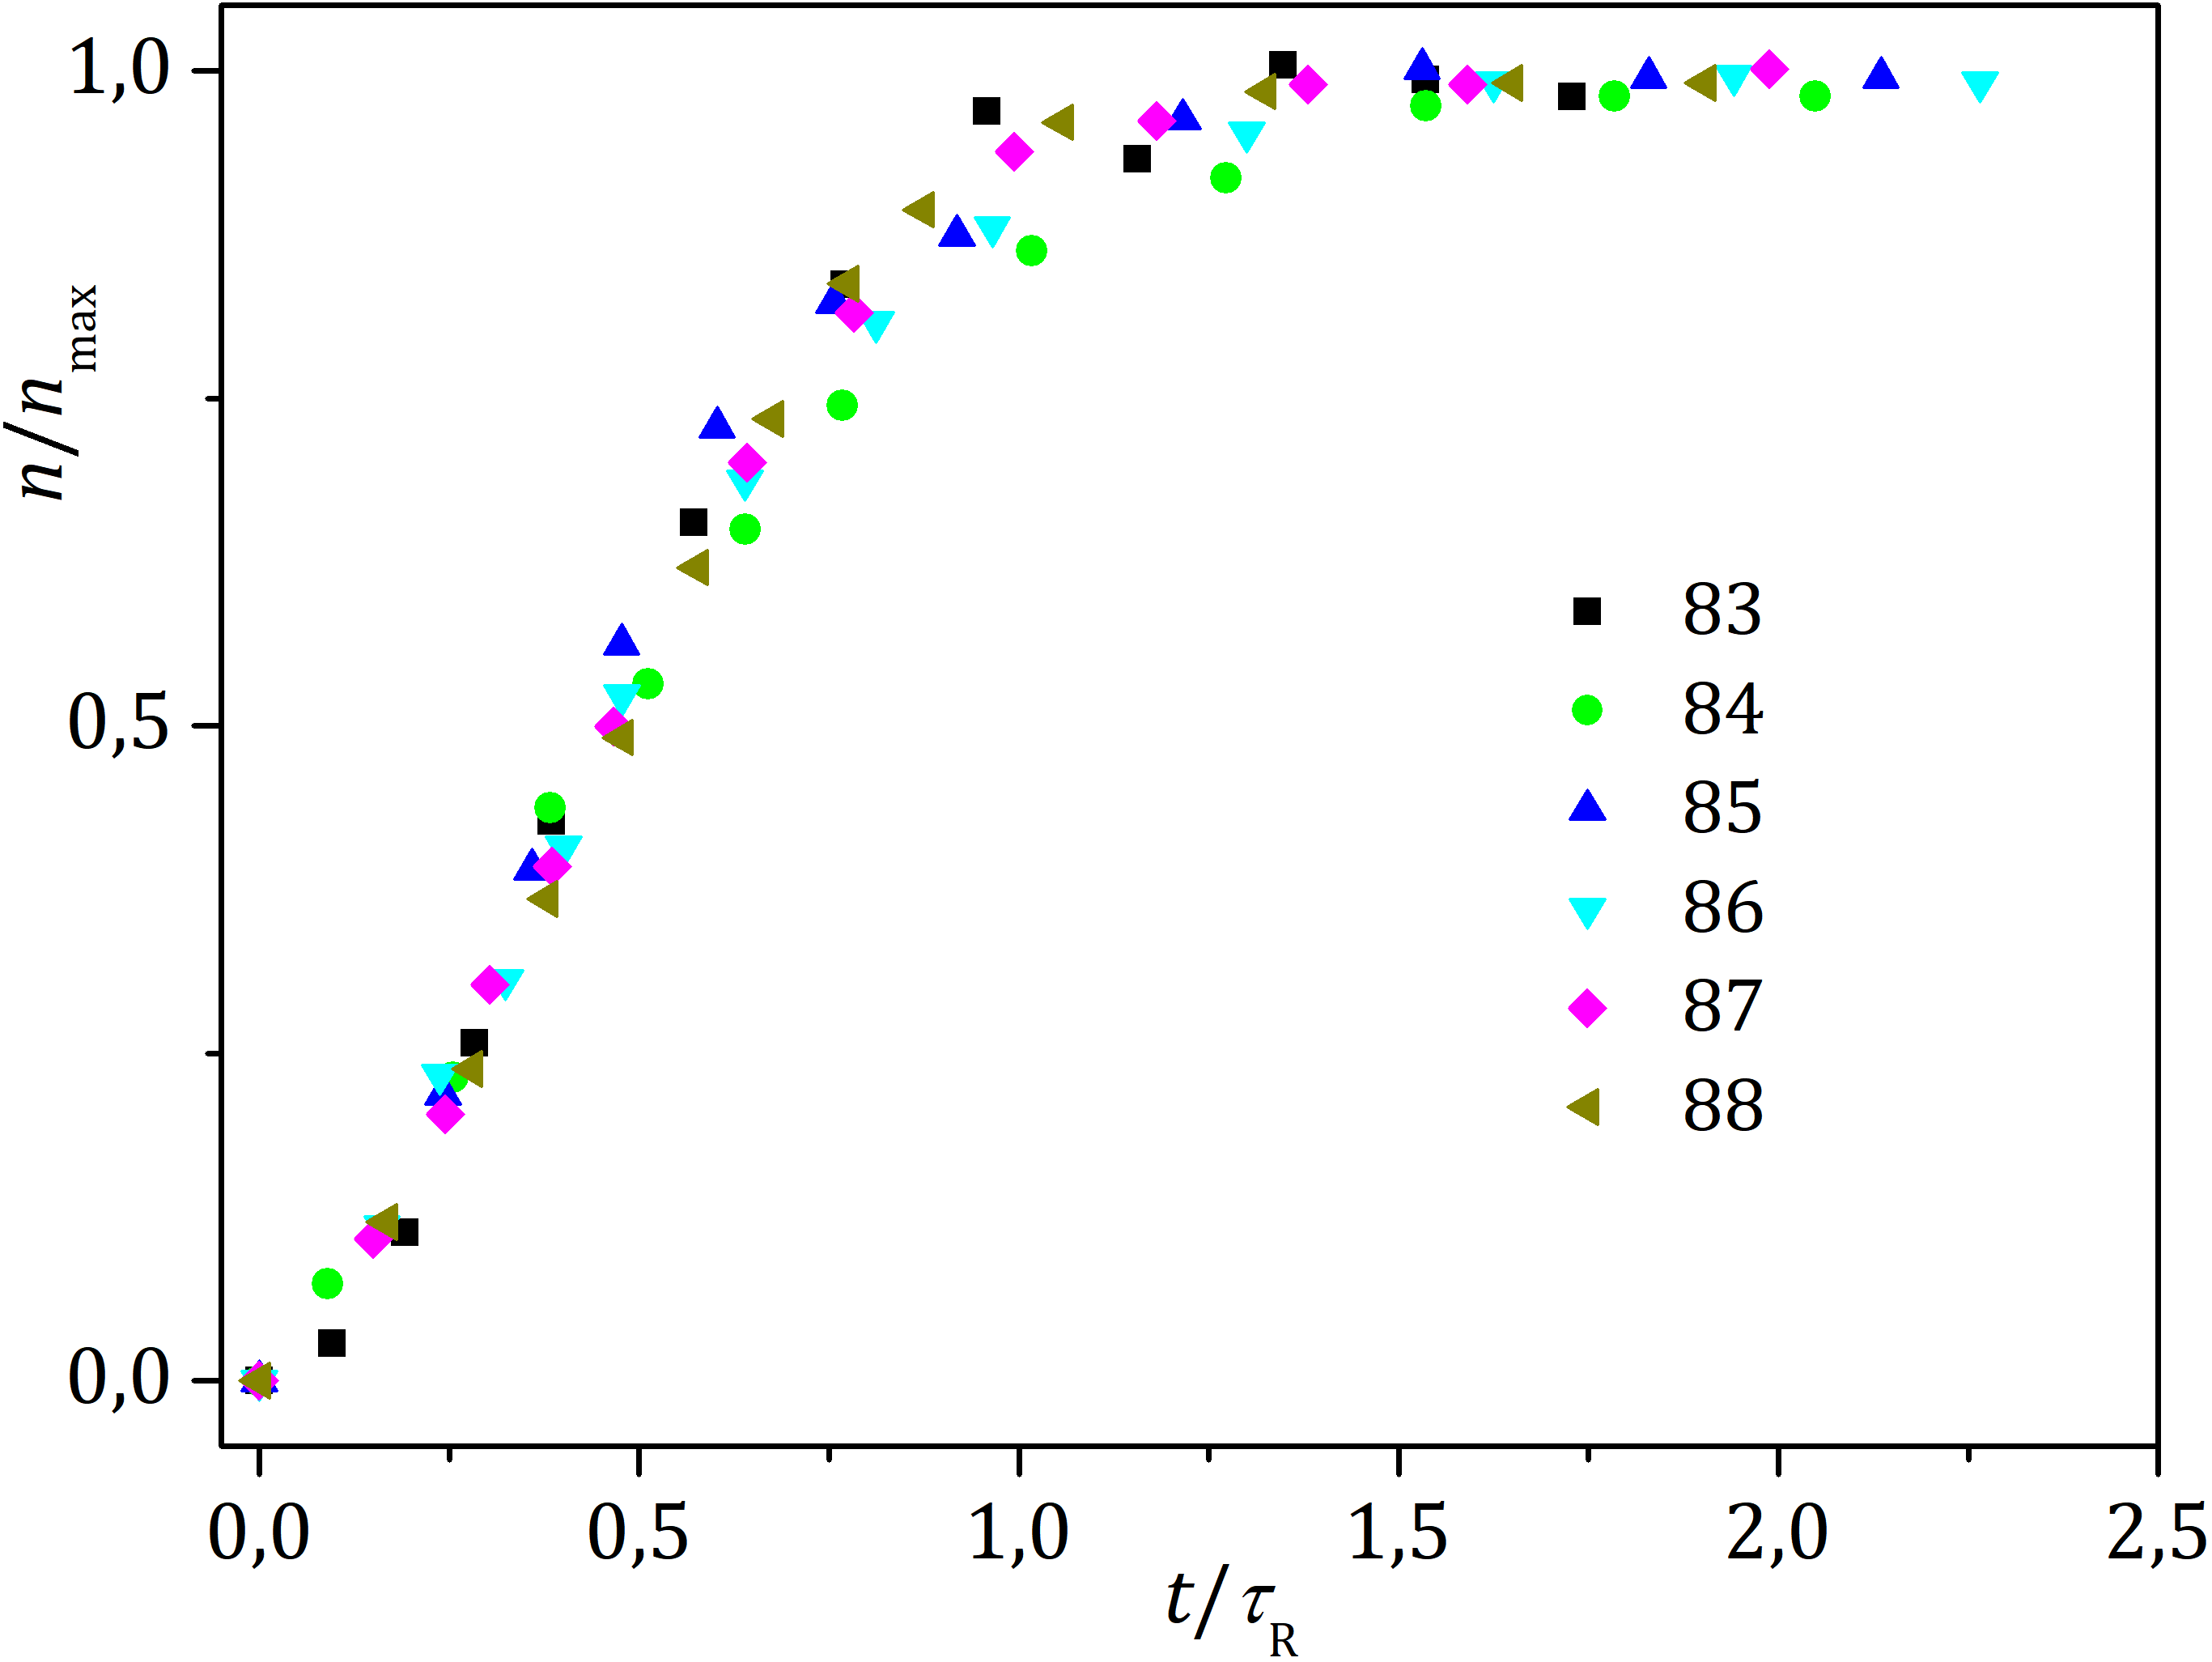
\includegraphics[width=0.43\textwidth]{ivan_markov_graphs/richards_rescaled_fig5.png}}
        \subfloat[Фиг. 6]{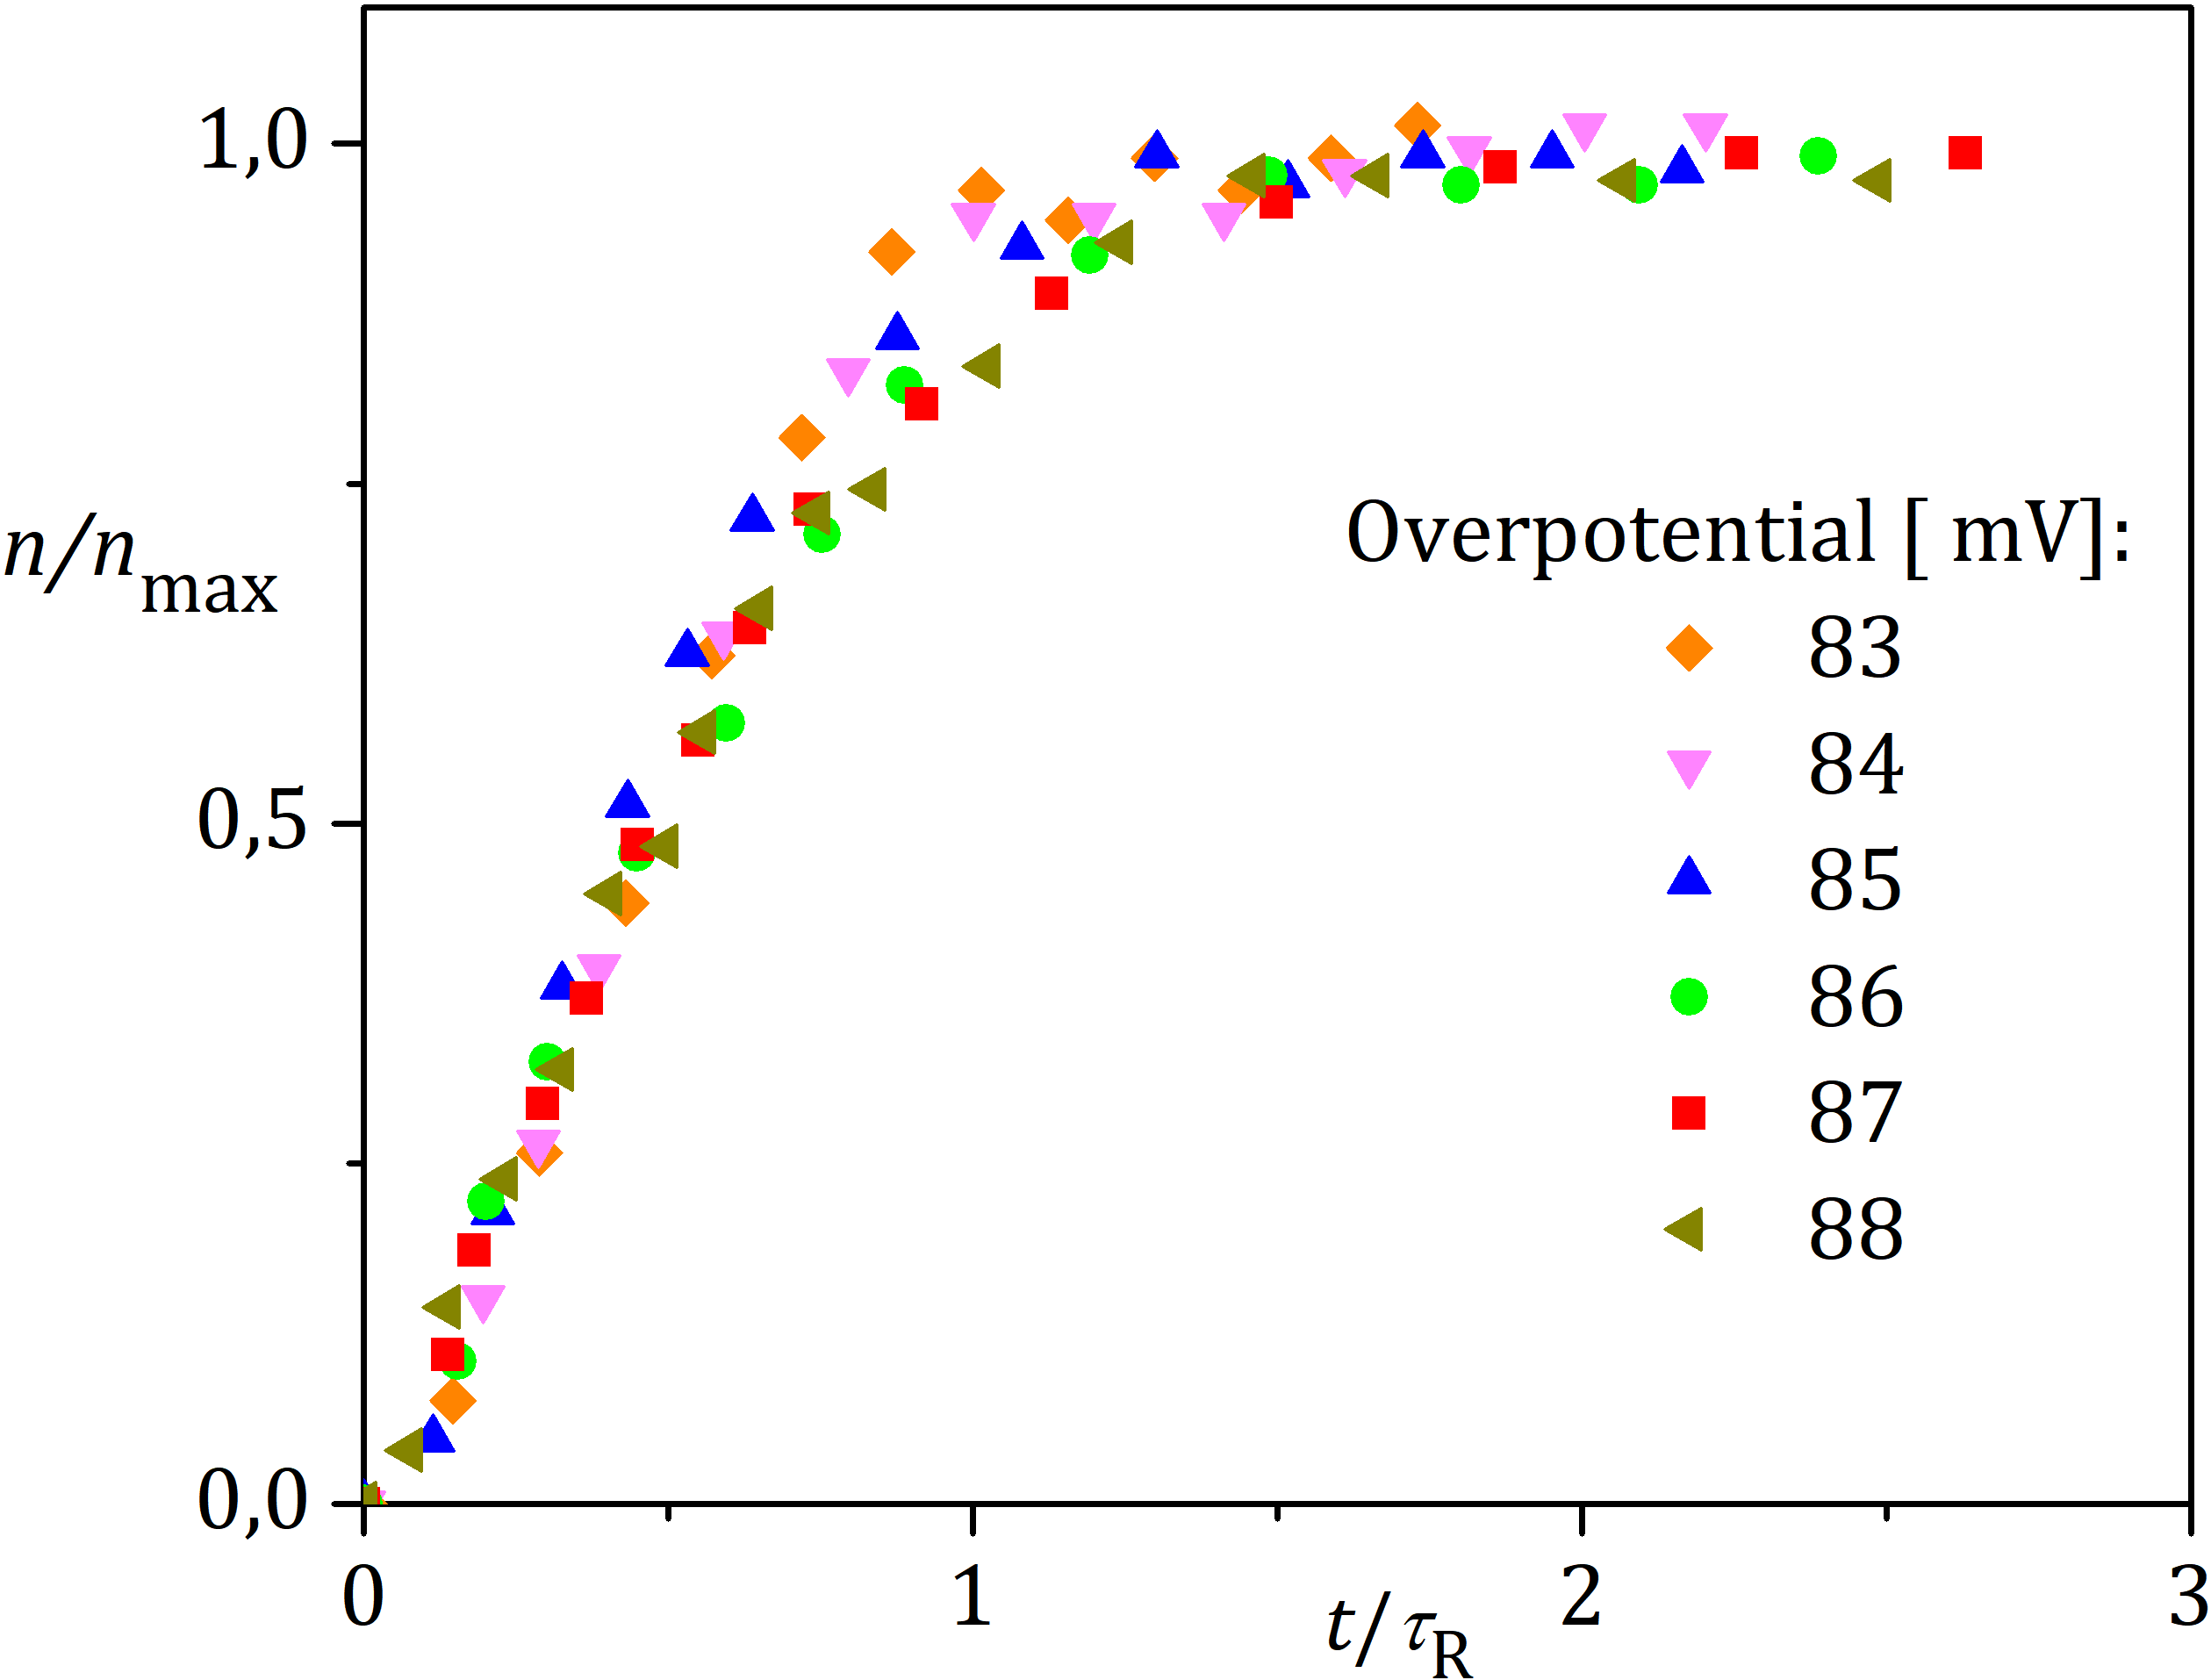
\includegraphics[width=0.43\textwidth]{ivan_markov_graphs/richards_rescaled_fig6.png}}
    \label{fig:richards_rescaled}
\end{figure}
\begin{figure}[H]
    \centering
        \subfloat[Фиг. 5]{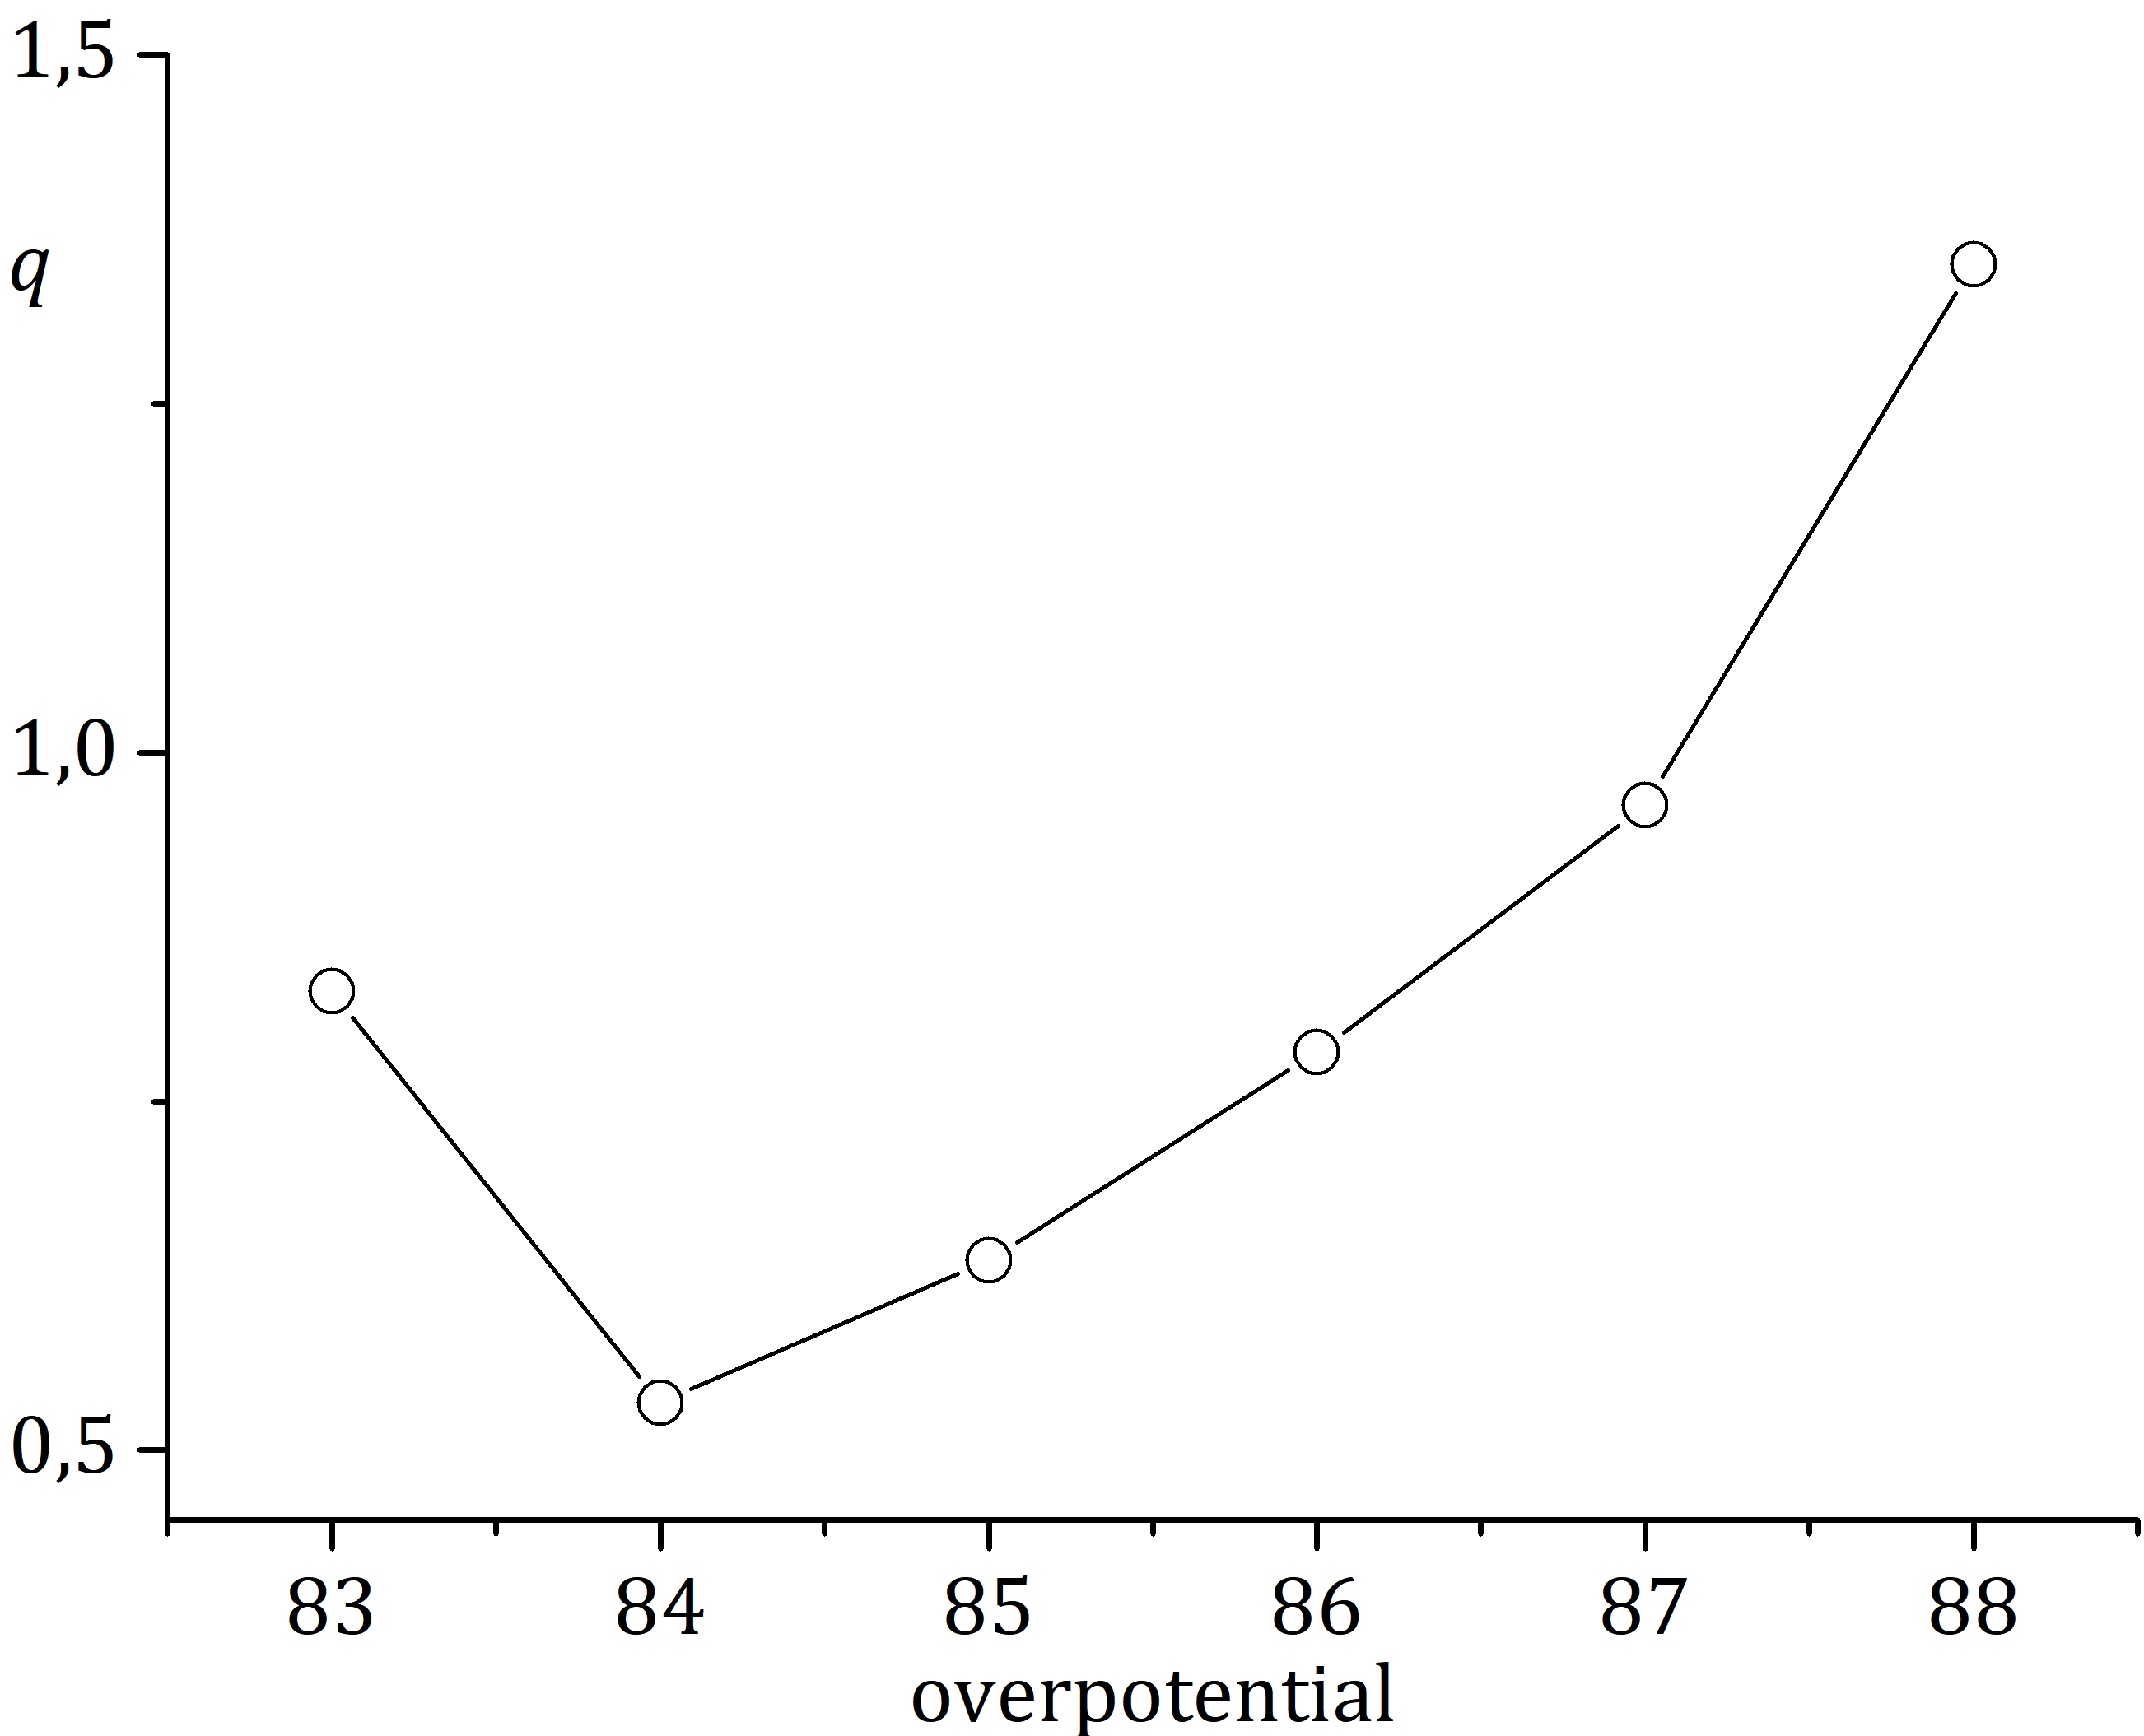
\includegraphics[width=0.38\textwidth]{ivan_markov_graphs/Fig5_q-overpotential.png}}
        \subfloat[Фиг. 6]{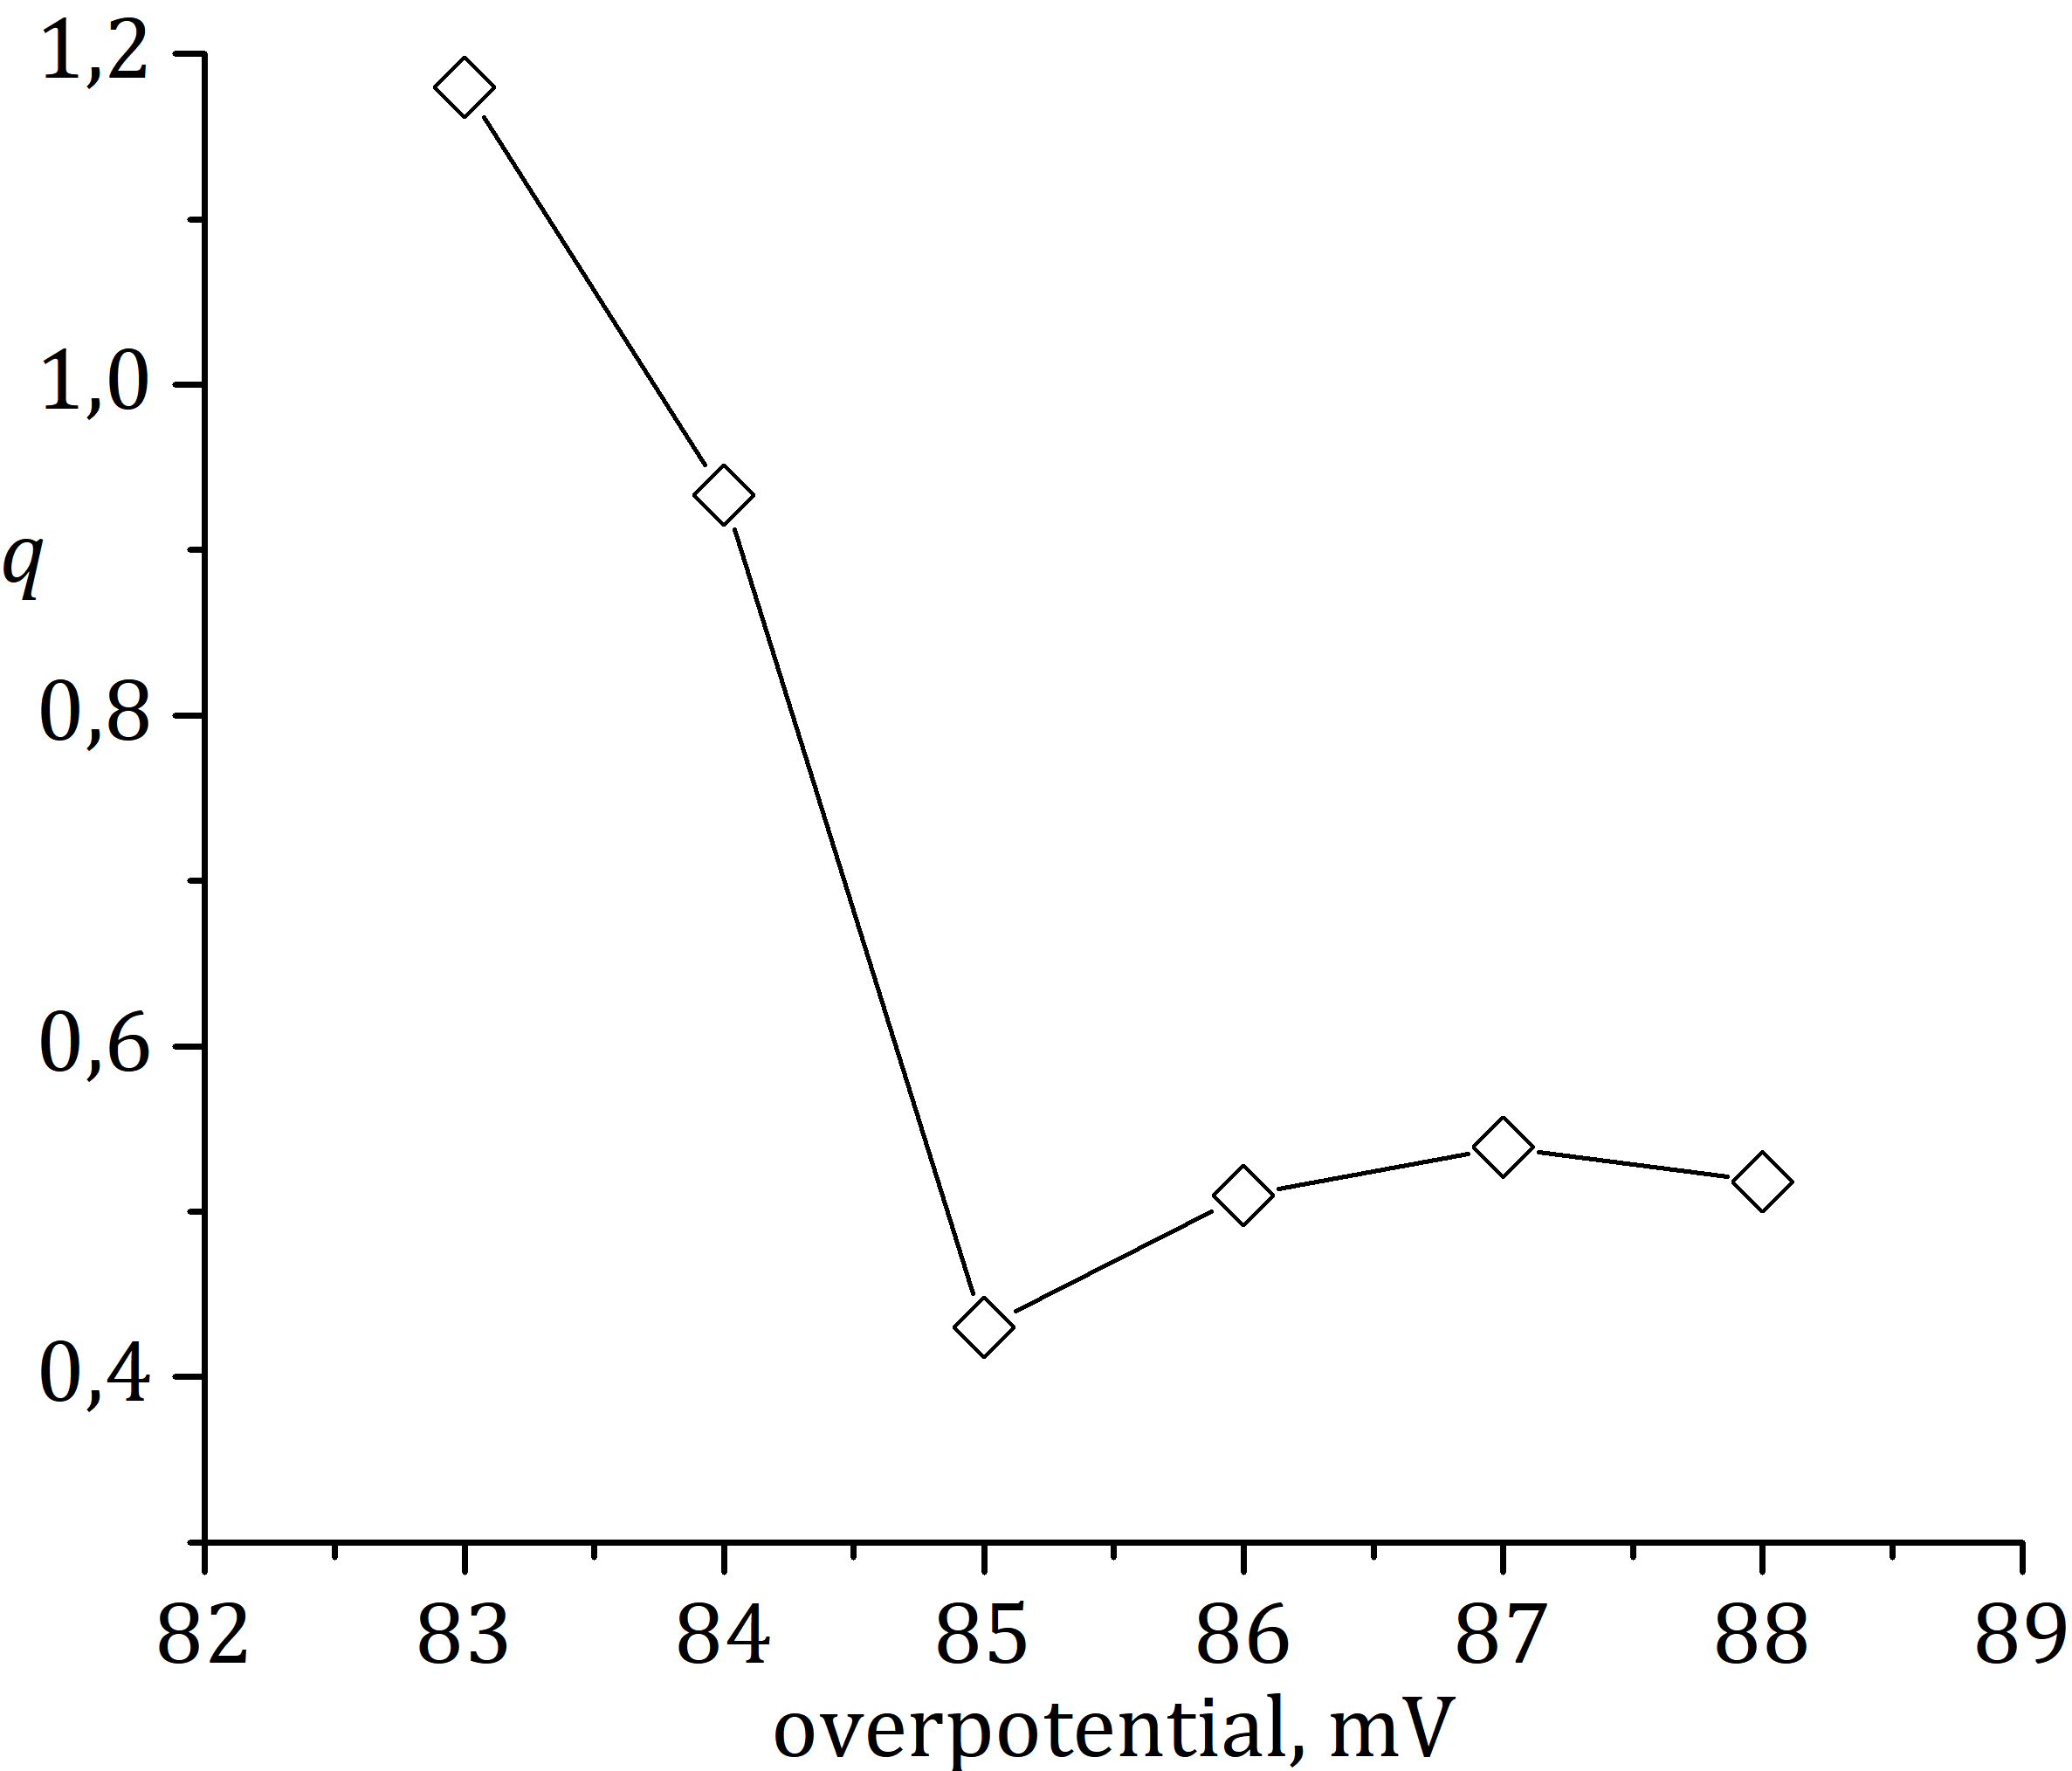
\includegraphics[width=0.38\textwidth]{ivan_markov_graphs/Fig6_q-overpotential.png}}
    \caption{Зависимост на параметъра $q$ от модела на Ричардс от свръхпотенциала (вж. също \cite{VikiPHD2023} \cite{ivanmarkovpreprint})}
\end{figure}
\begin{figure}[H]
    \centering
        \subfloat[Фиг. 5]{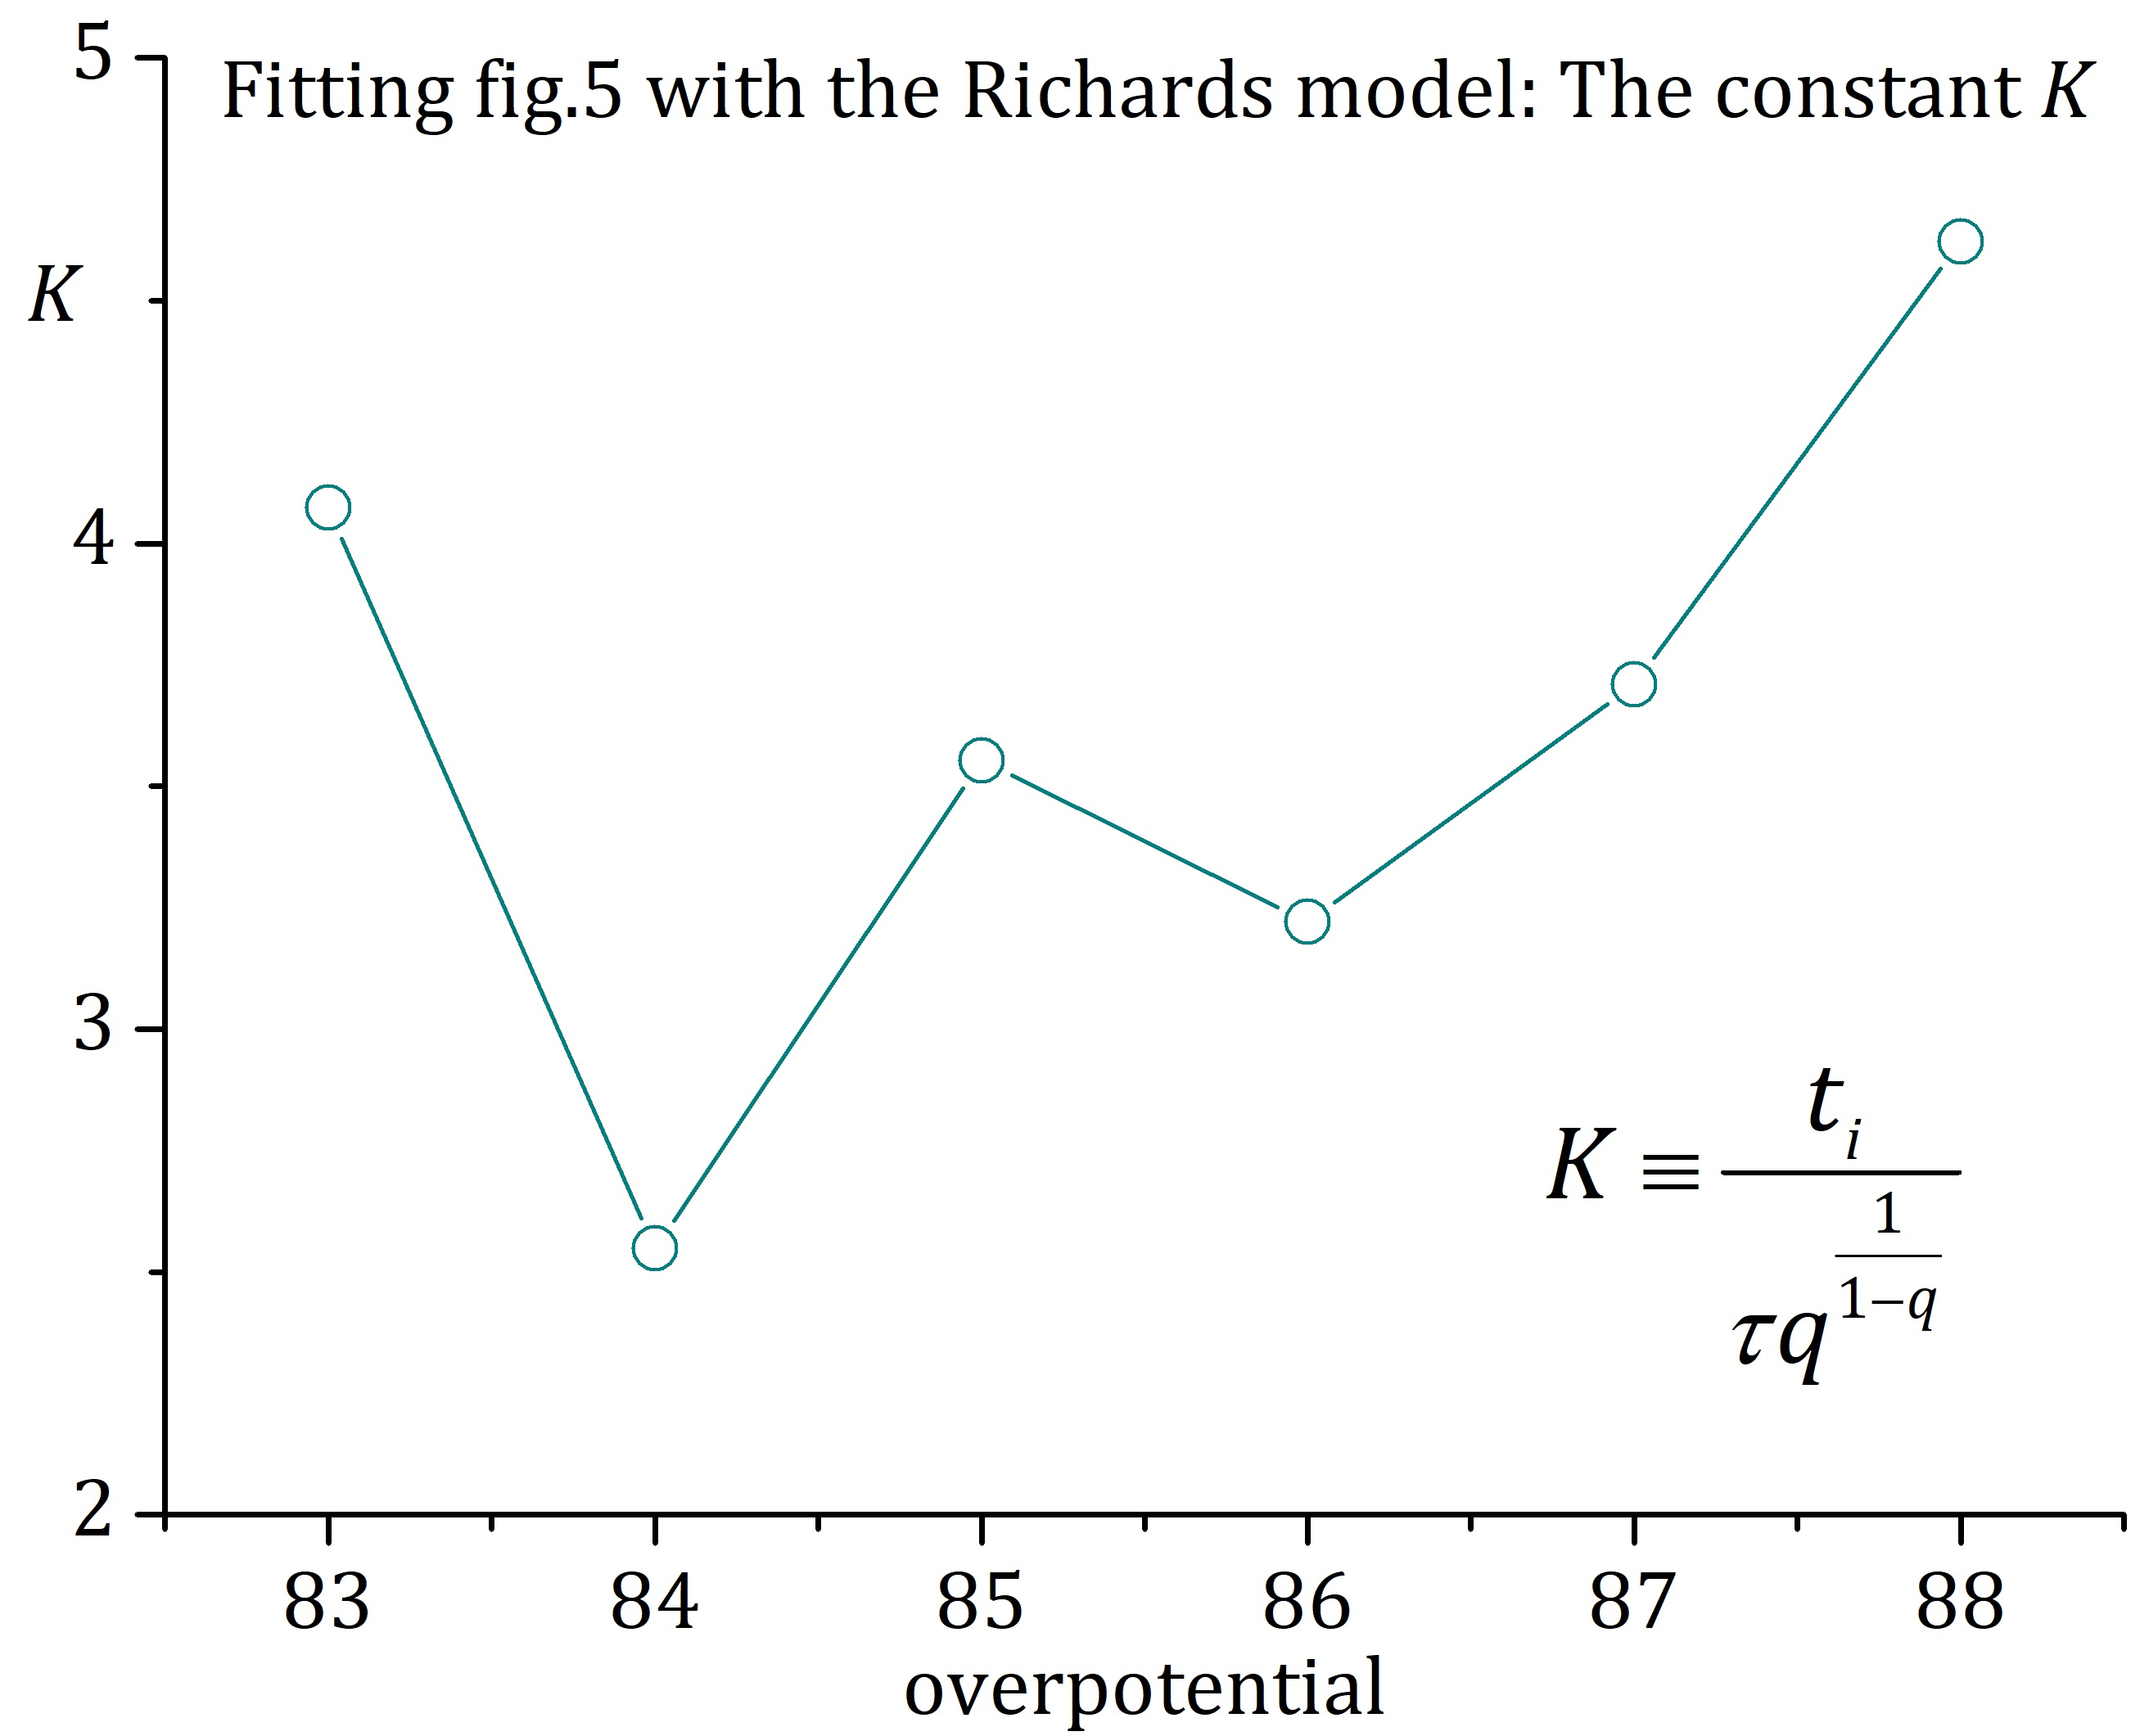
\includegraphics[width=0.45\textwidth]{ivan_markov_graphs/Fig5_K-overpotential.jpg}}
        \subfloat[Фиг. 6]{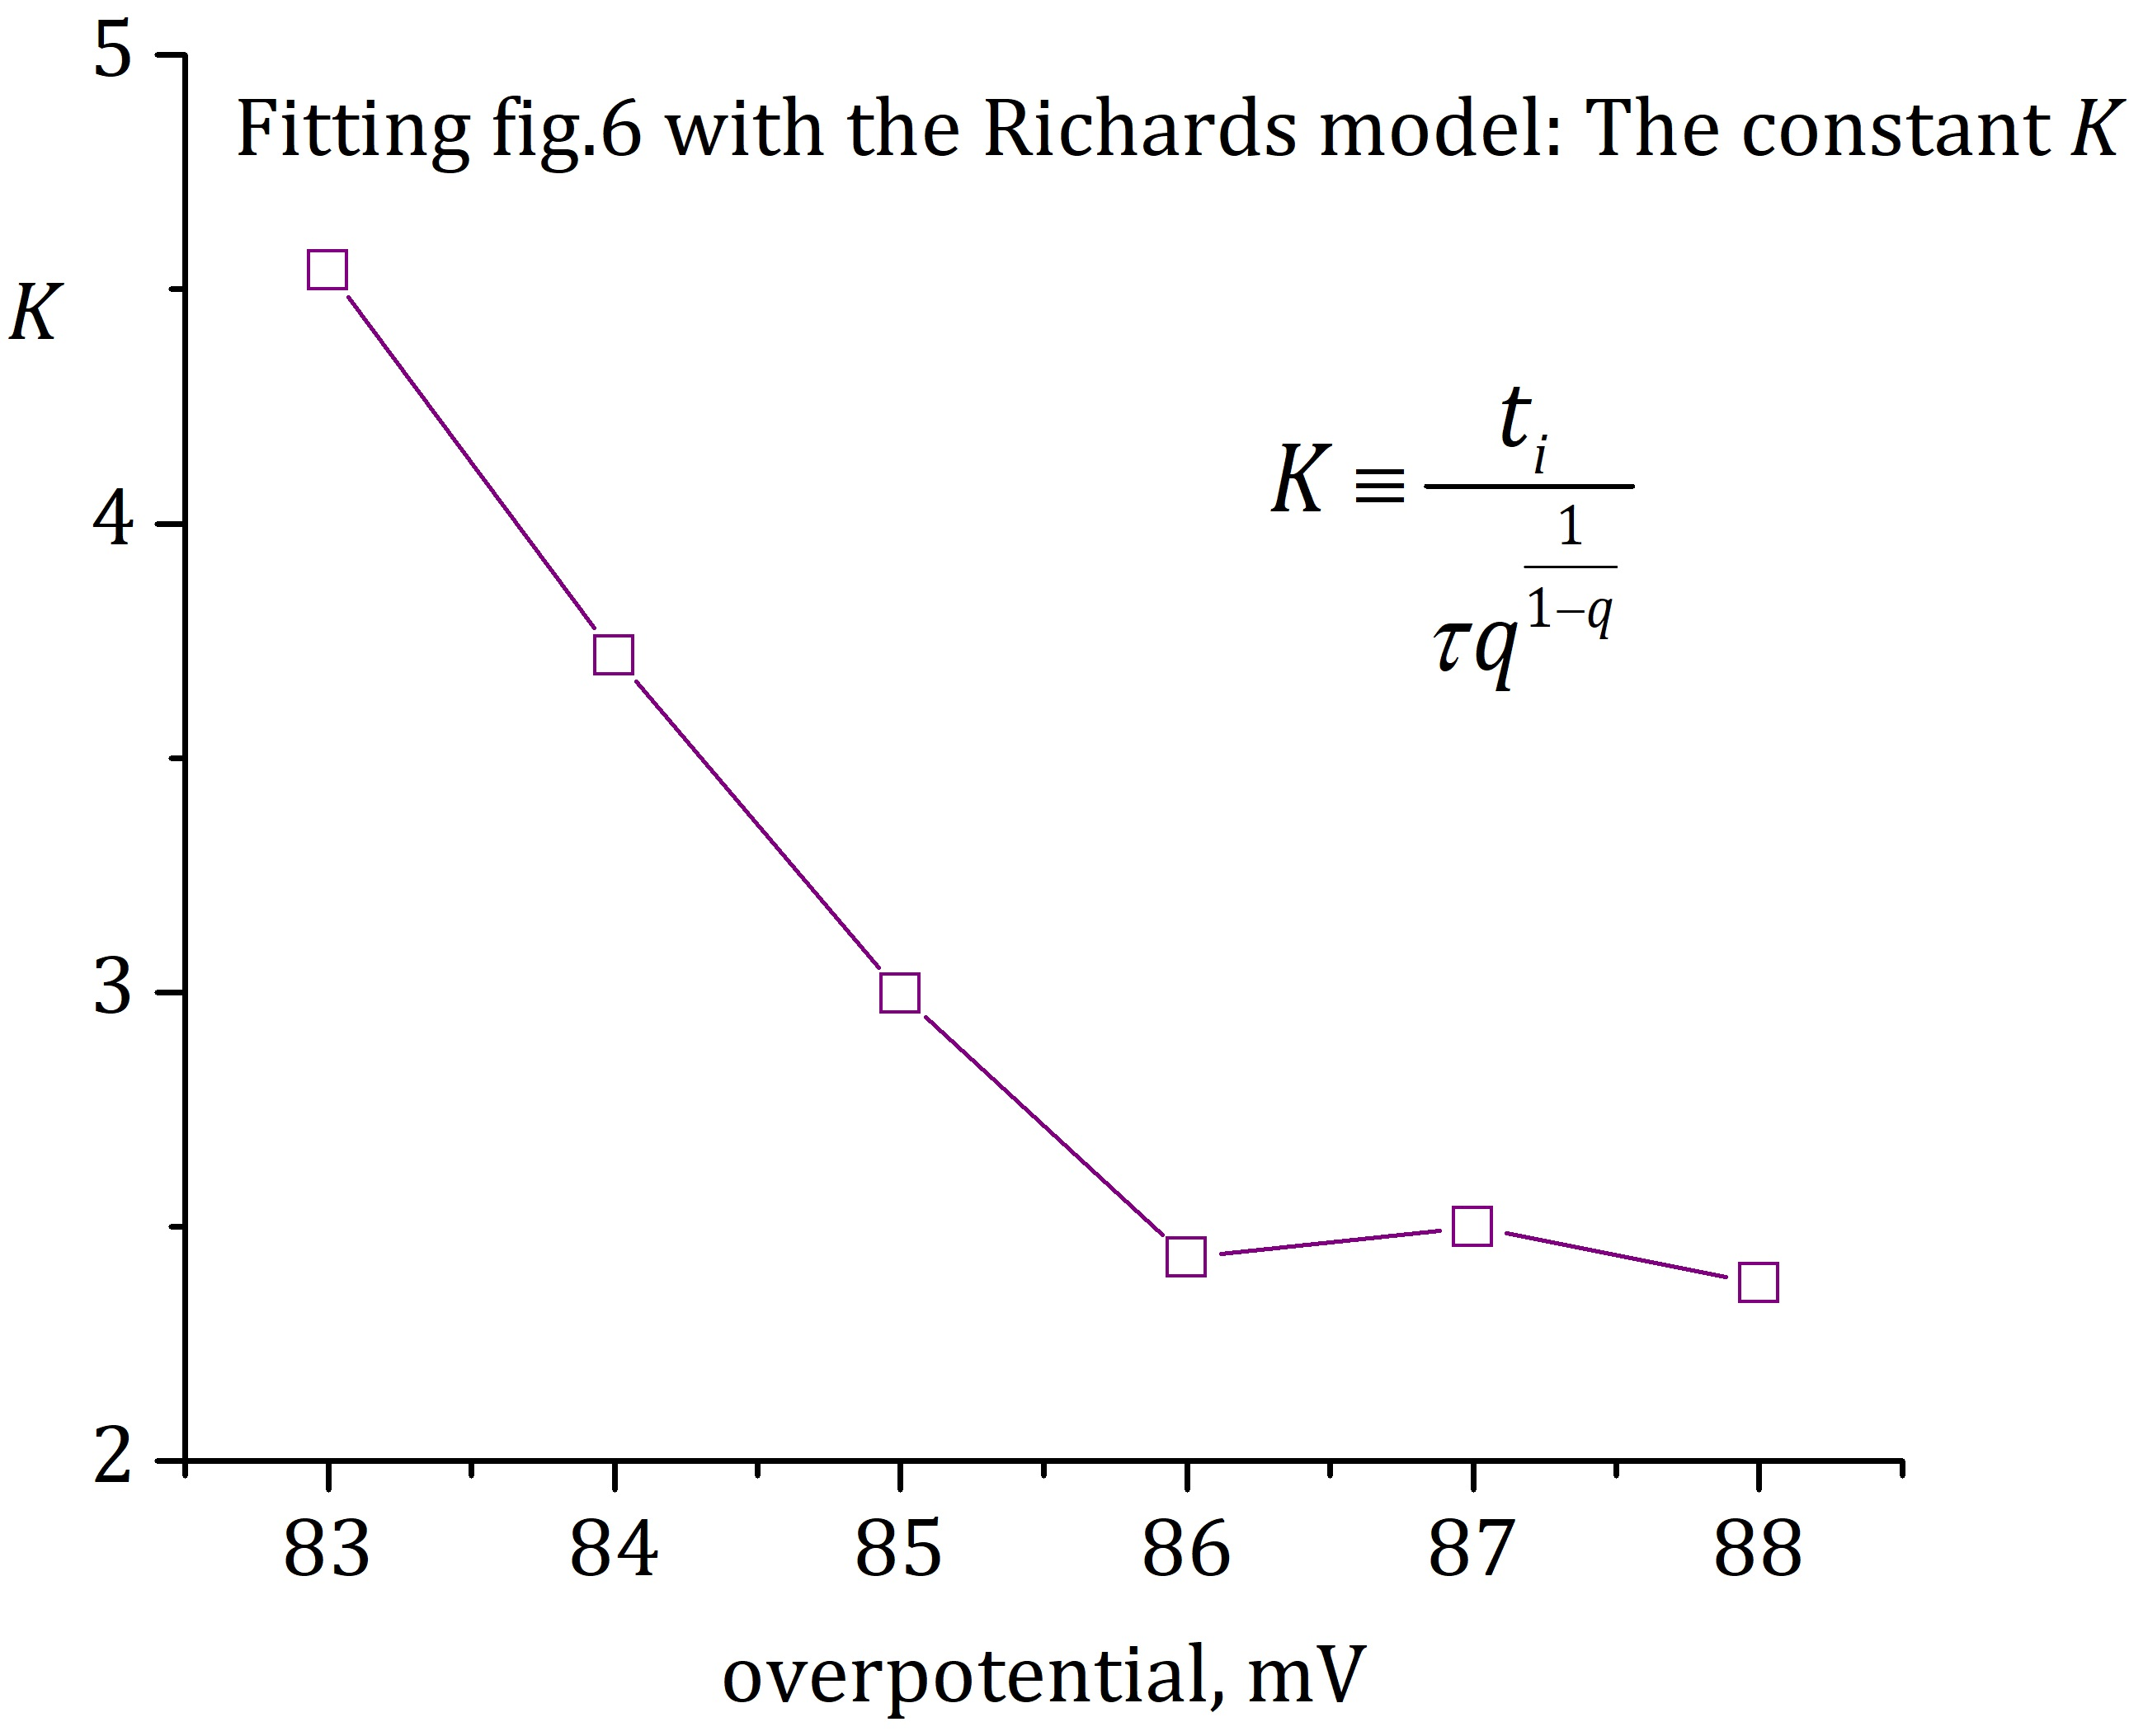
\includegraphics[width=0.45\textwidth]{ivan_markov_graphs/Fig6_K-overpotential.jpg}}
    \caption{Зависимост на параметъра $K$ от модела на Ричардс от свръхпотенциала}
\end{figure}

Важно е да отбележим, че на \autoref{fig:richards_rescaled} няма универсална крива, тъй като параметрите $q, K$ на модела са различни за всеки набор данни.
\subsubsection{Модел JMAKn}
\begin{figure}[H]
    \centering
        \subfloat[Фиг. 5]{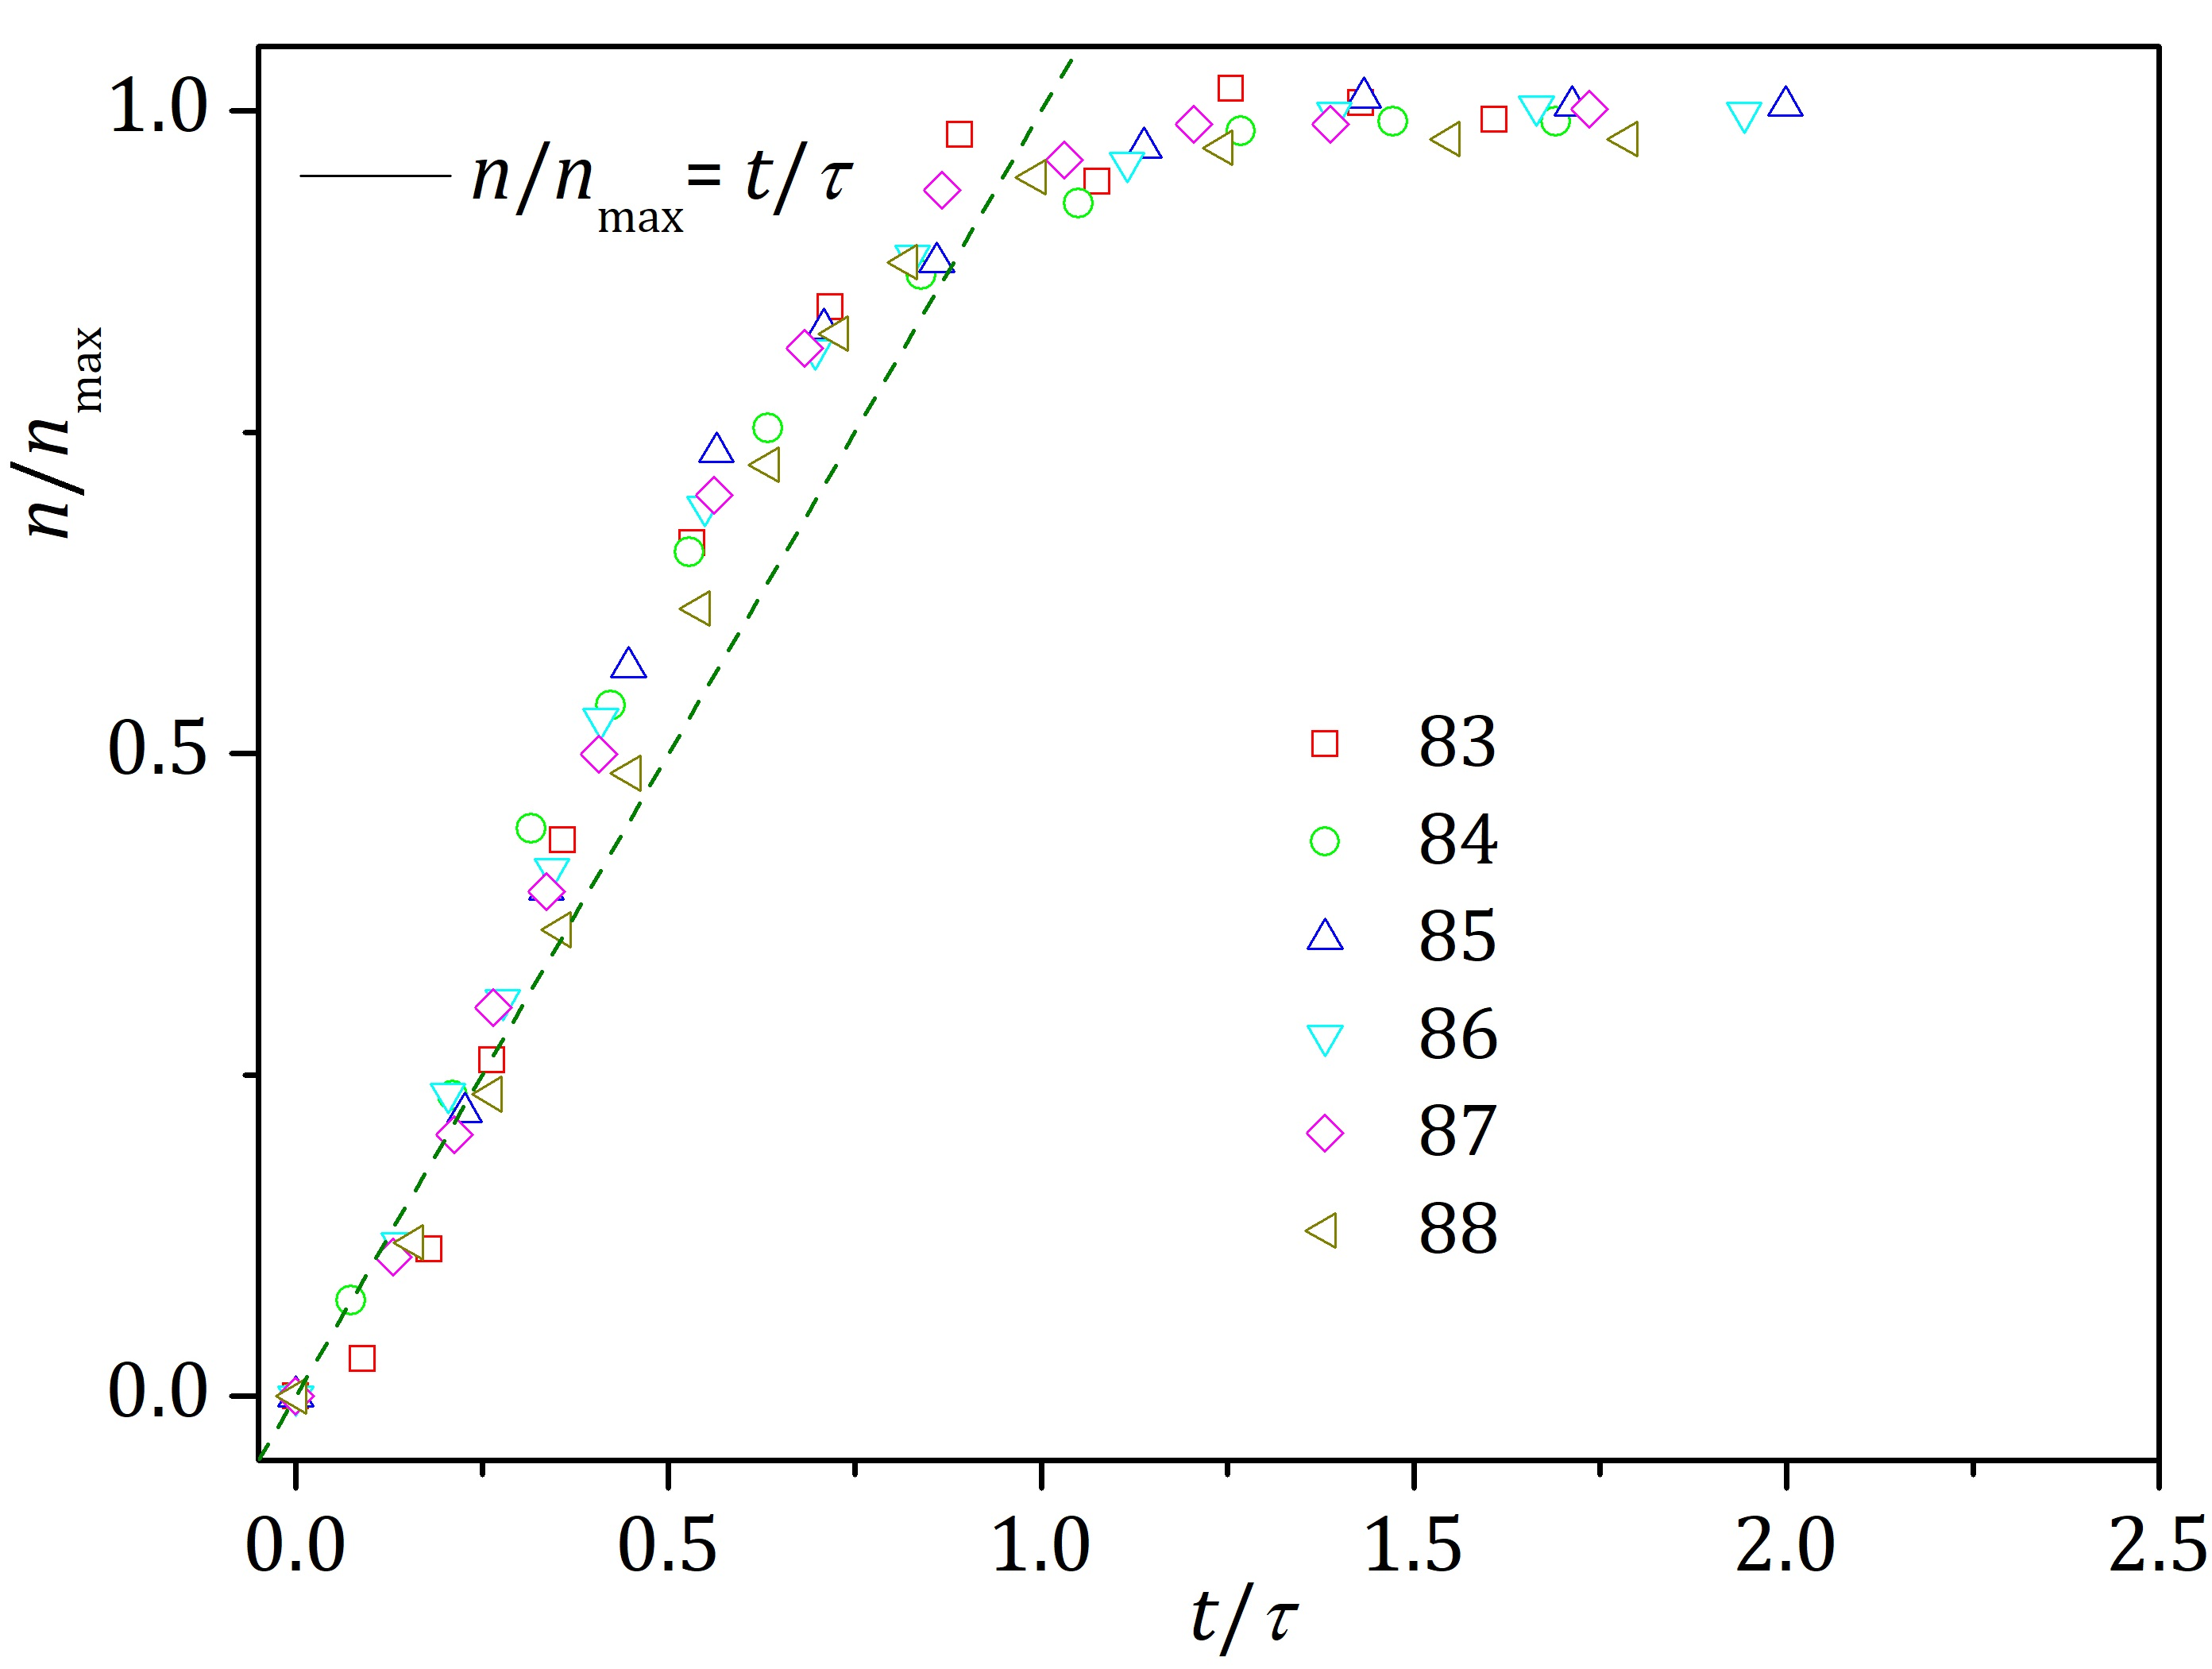
\includegraphics[width=0.48\textwidth]{ivan_markov_graphs/Fig5-jmak_rescaled.jpg}}
        \subfloat[Фиг. 6]{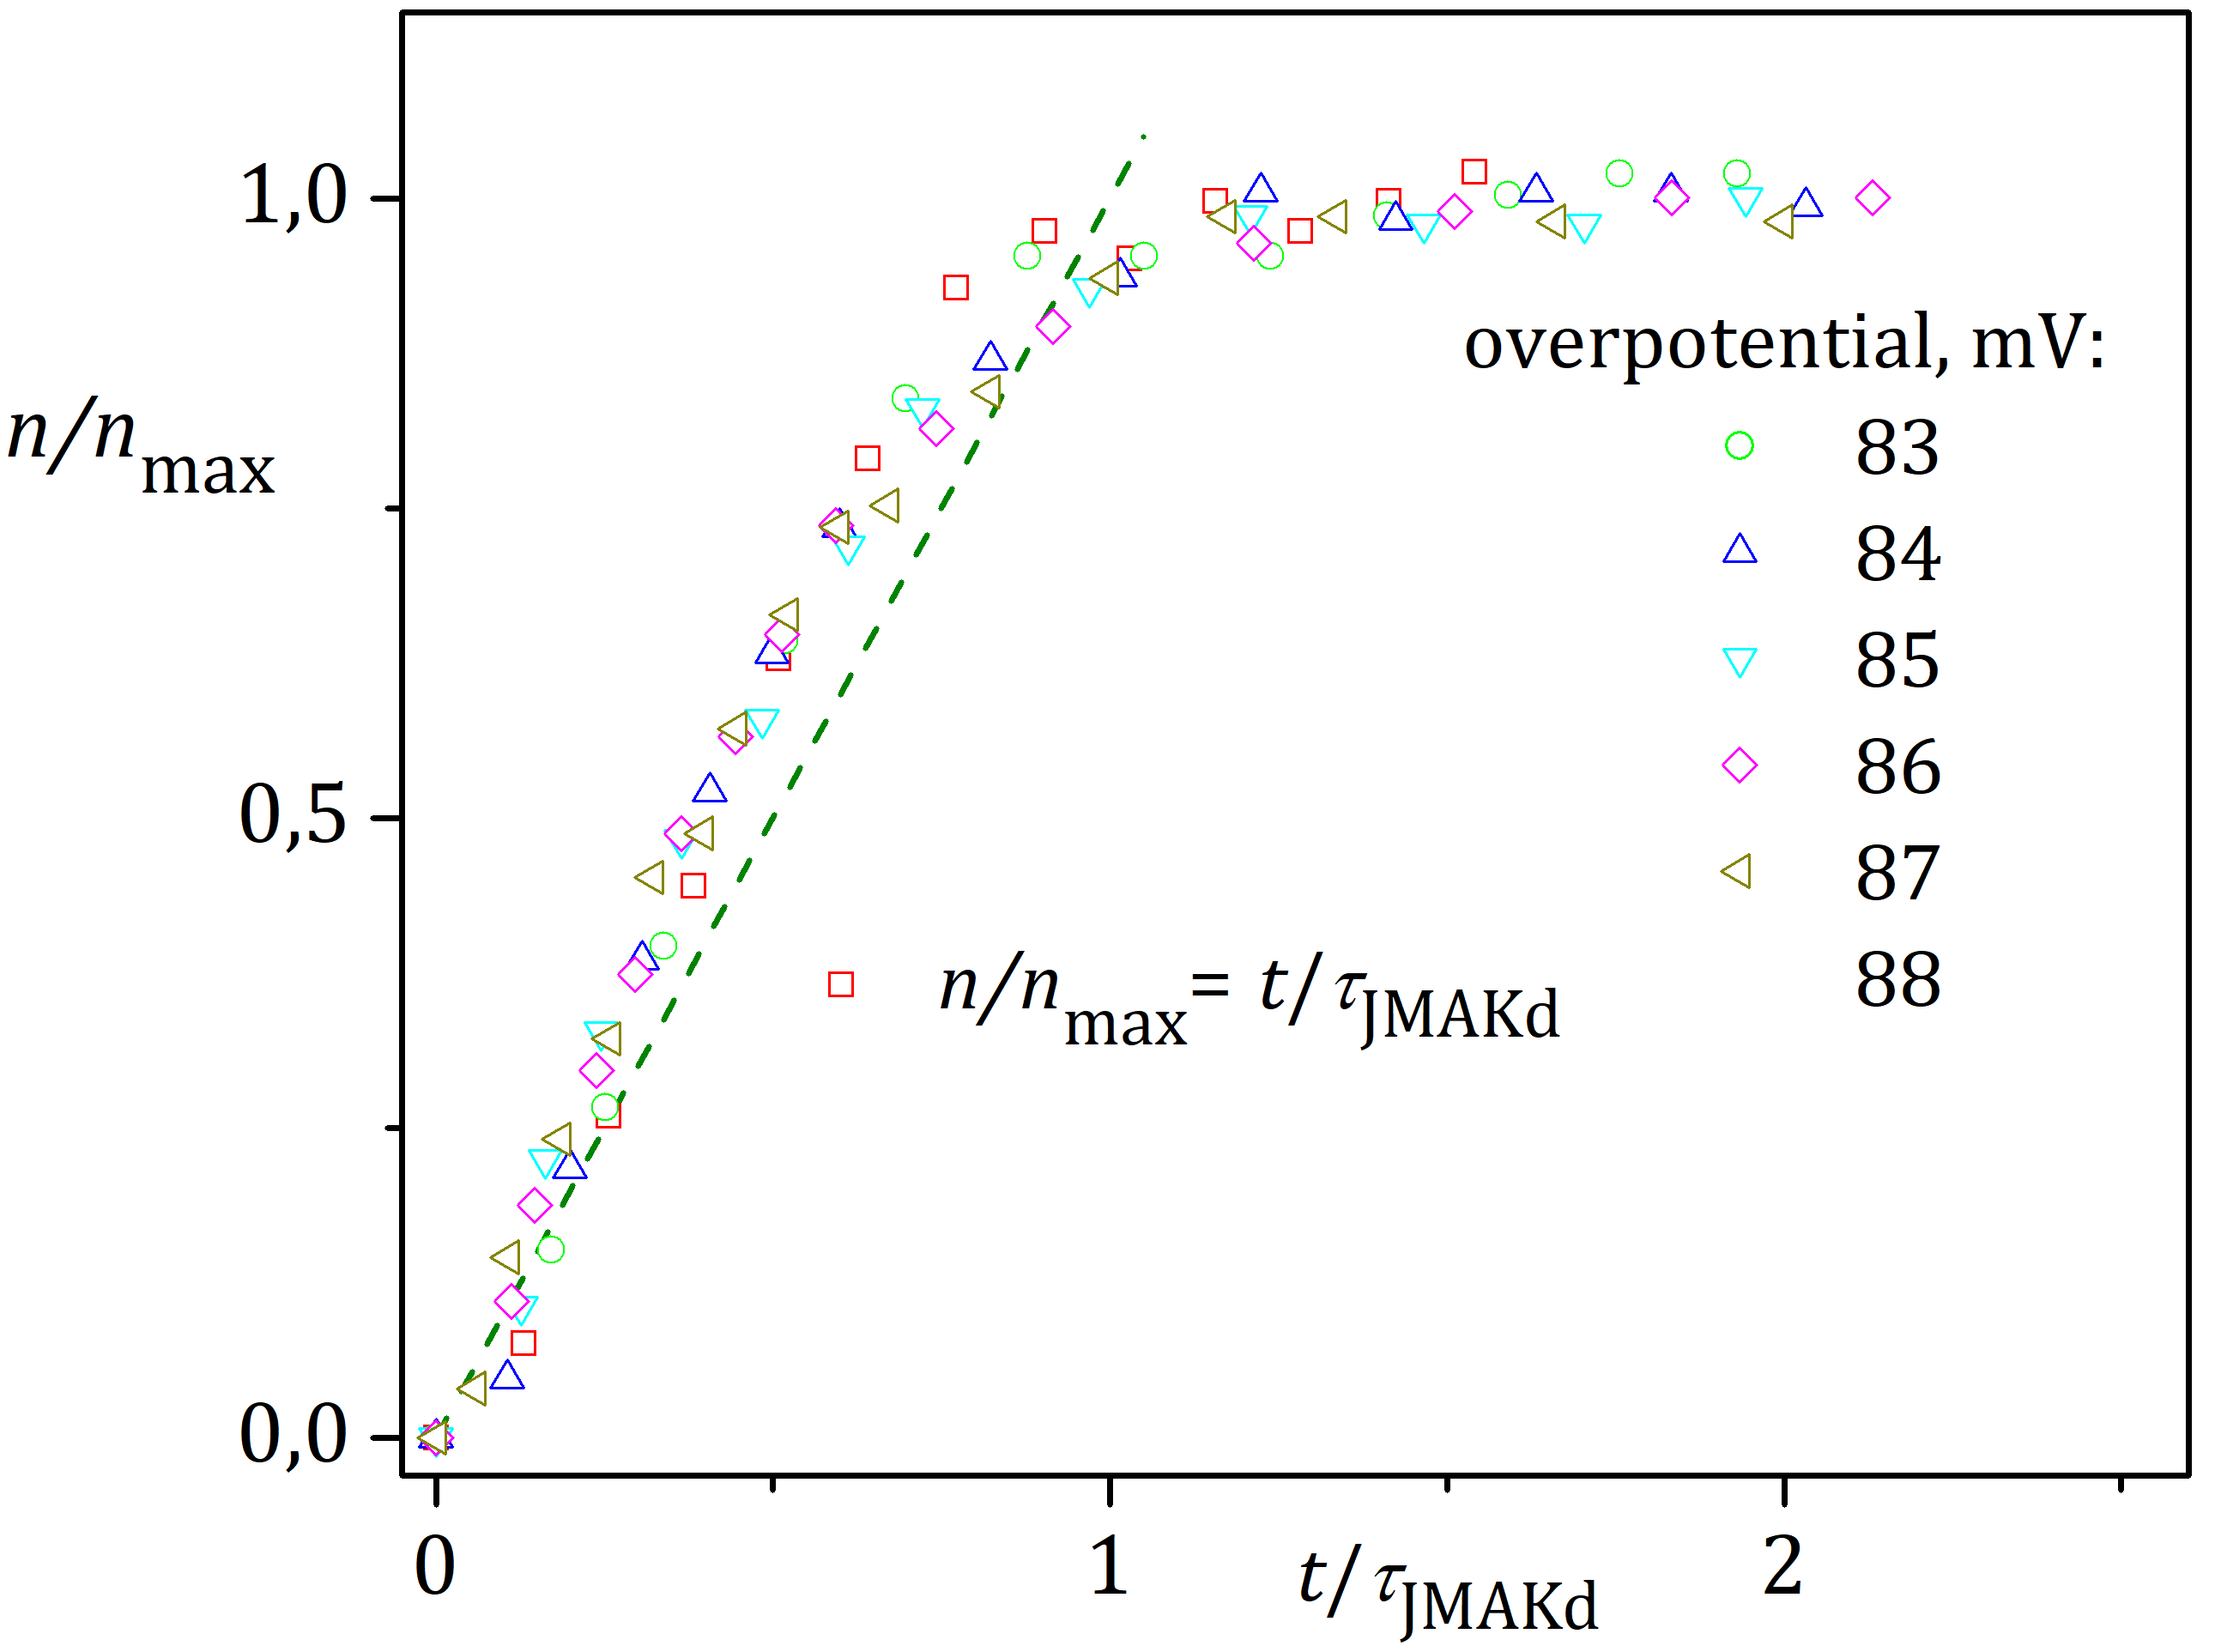
\includegraphics[width=0.48\textwidth]{ivan_markov_graphs/Fig6-jmak_rescaled.png}}
    \caption{Рескалирани данни от JMAKn за различни свръхпотенциали}
\end{figure}
%% TODO: ADD REFERENCE TO TABLE WITH DATA!!!!

Тук отново нямаме универсална крива, тъй като за различните набори данни $n$ е различно. Стойността им е в интервала $n \in [1.6, 1.9]$, т.е. $n \approx 2$. Това потвърждава в комбинация с \autoref{fig:nvsd_graph} изборът ни за $\alpha_{21}$ като най-прост модел, съдържащ само $N_{max}$ и времева скала като параметри.
%% TODO: FIX d to be n on graph!!!!!!!
\begin{figure}[H]
    \centering
        \subfloat[Фиг. 5]{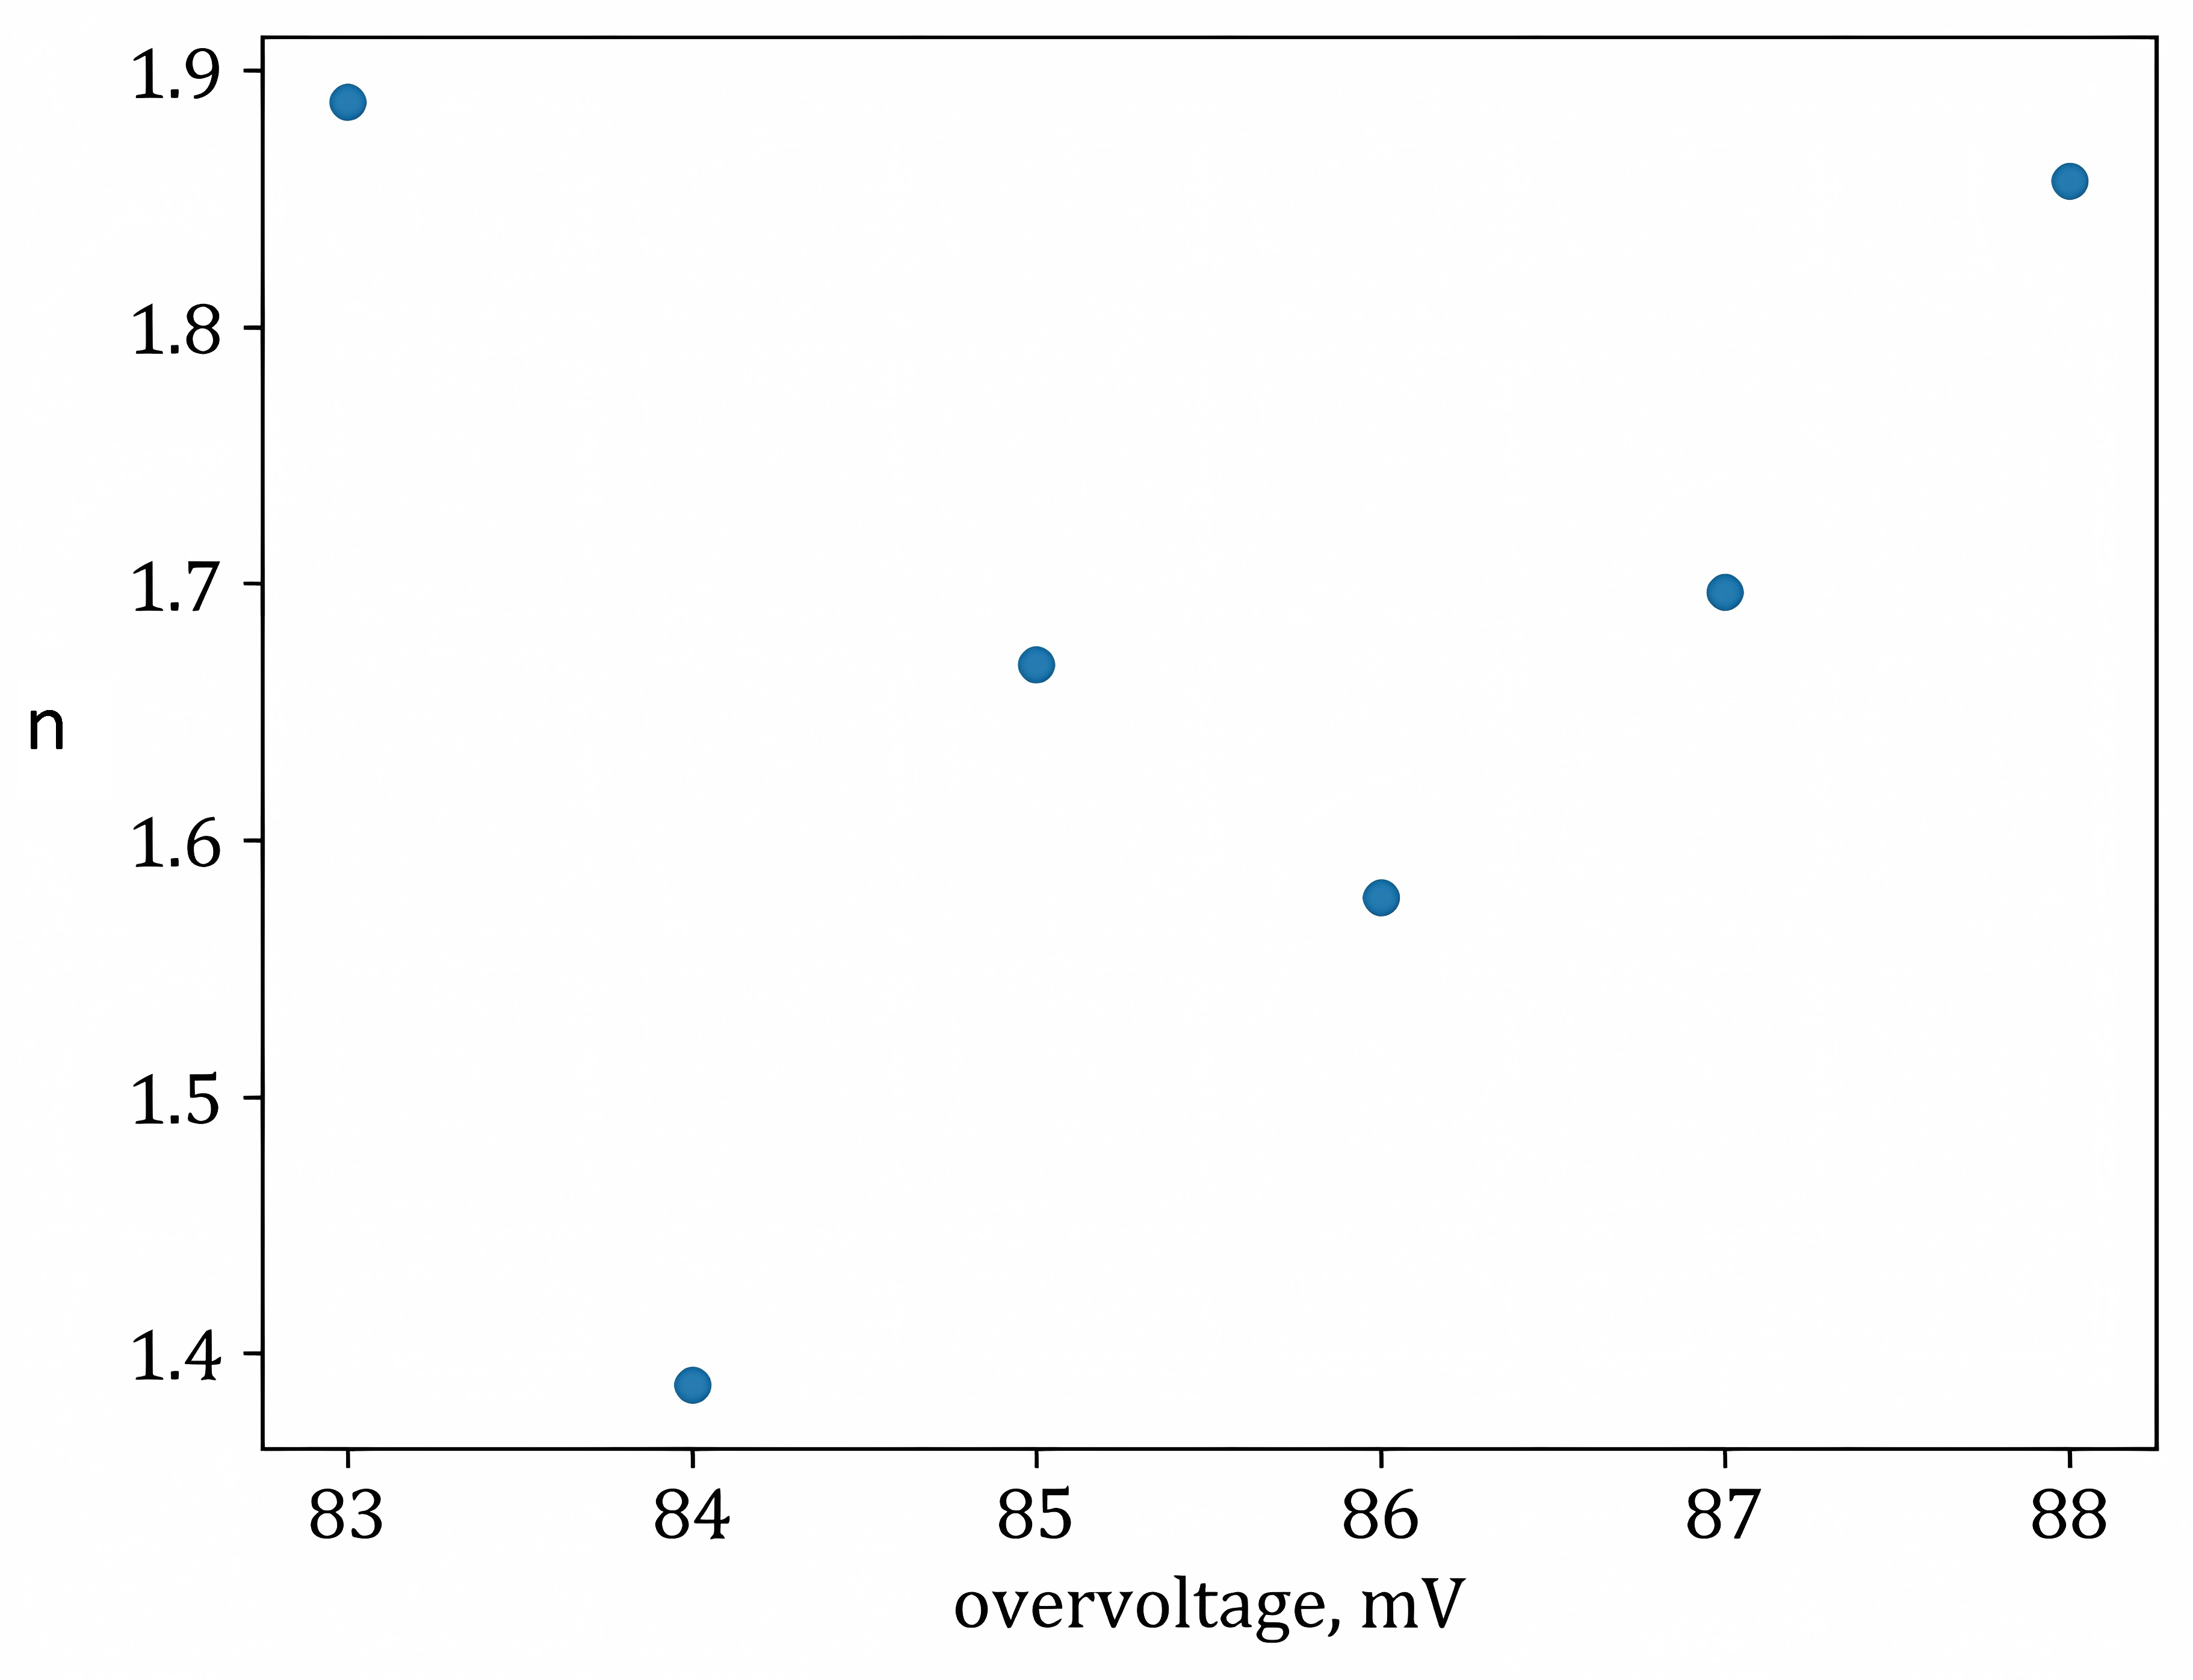
\includegraphics[width=0.48\textwidth]{ivan_markov_graphs/fig5_d_jmakn.png}}
        \subfloat[Фиг. 6]{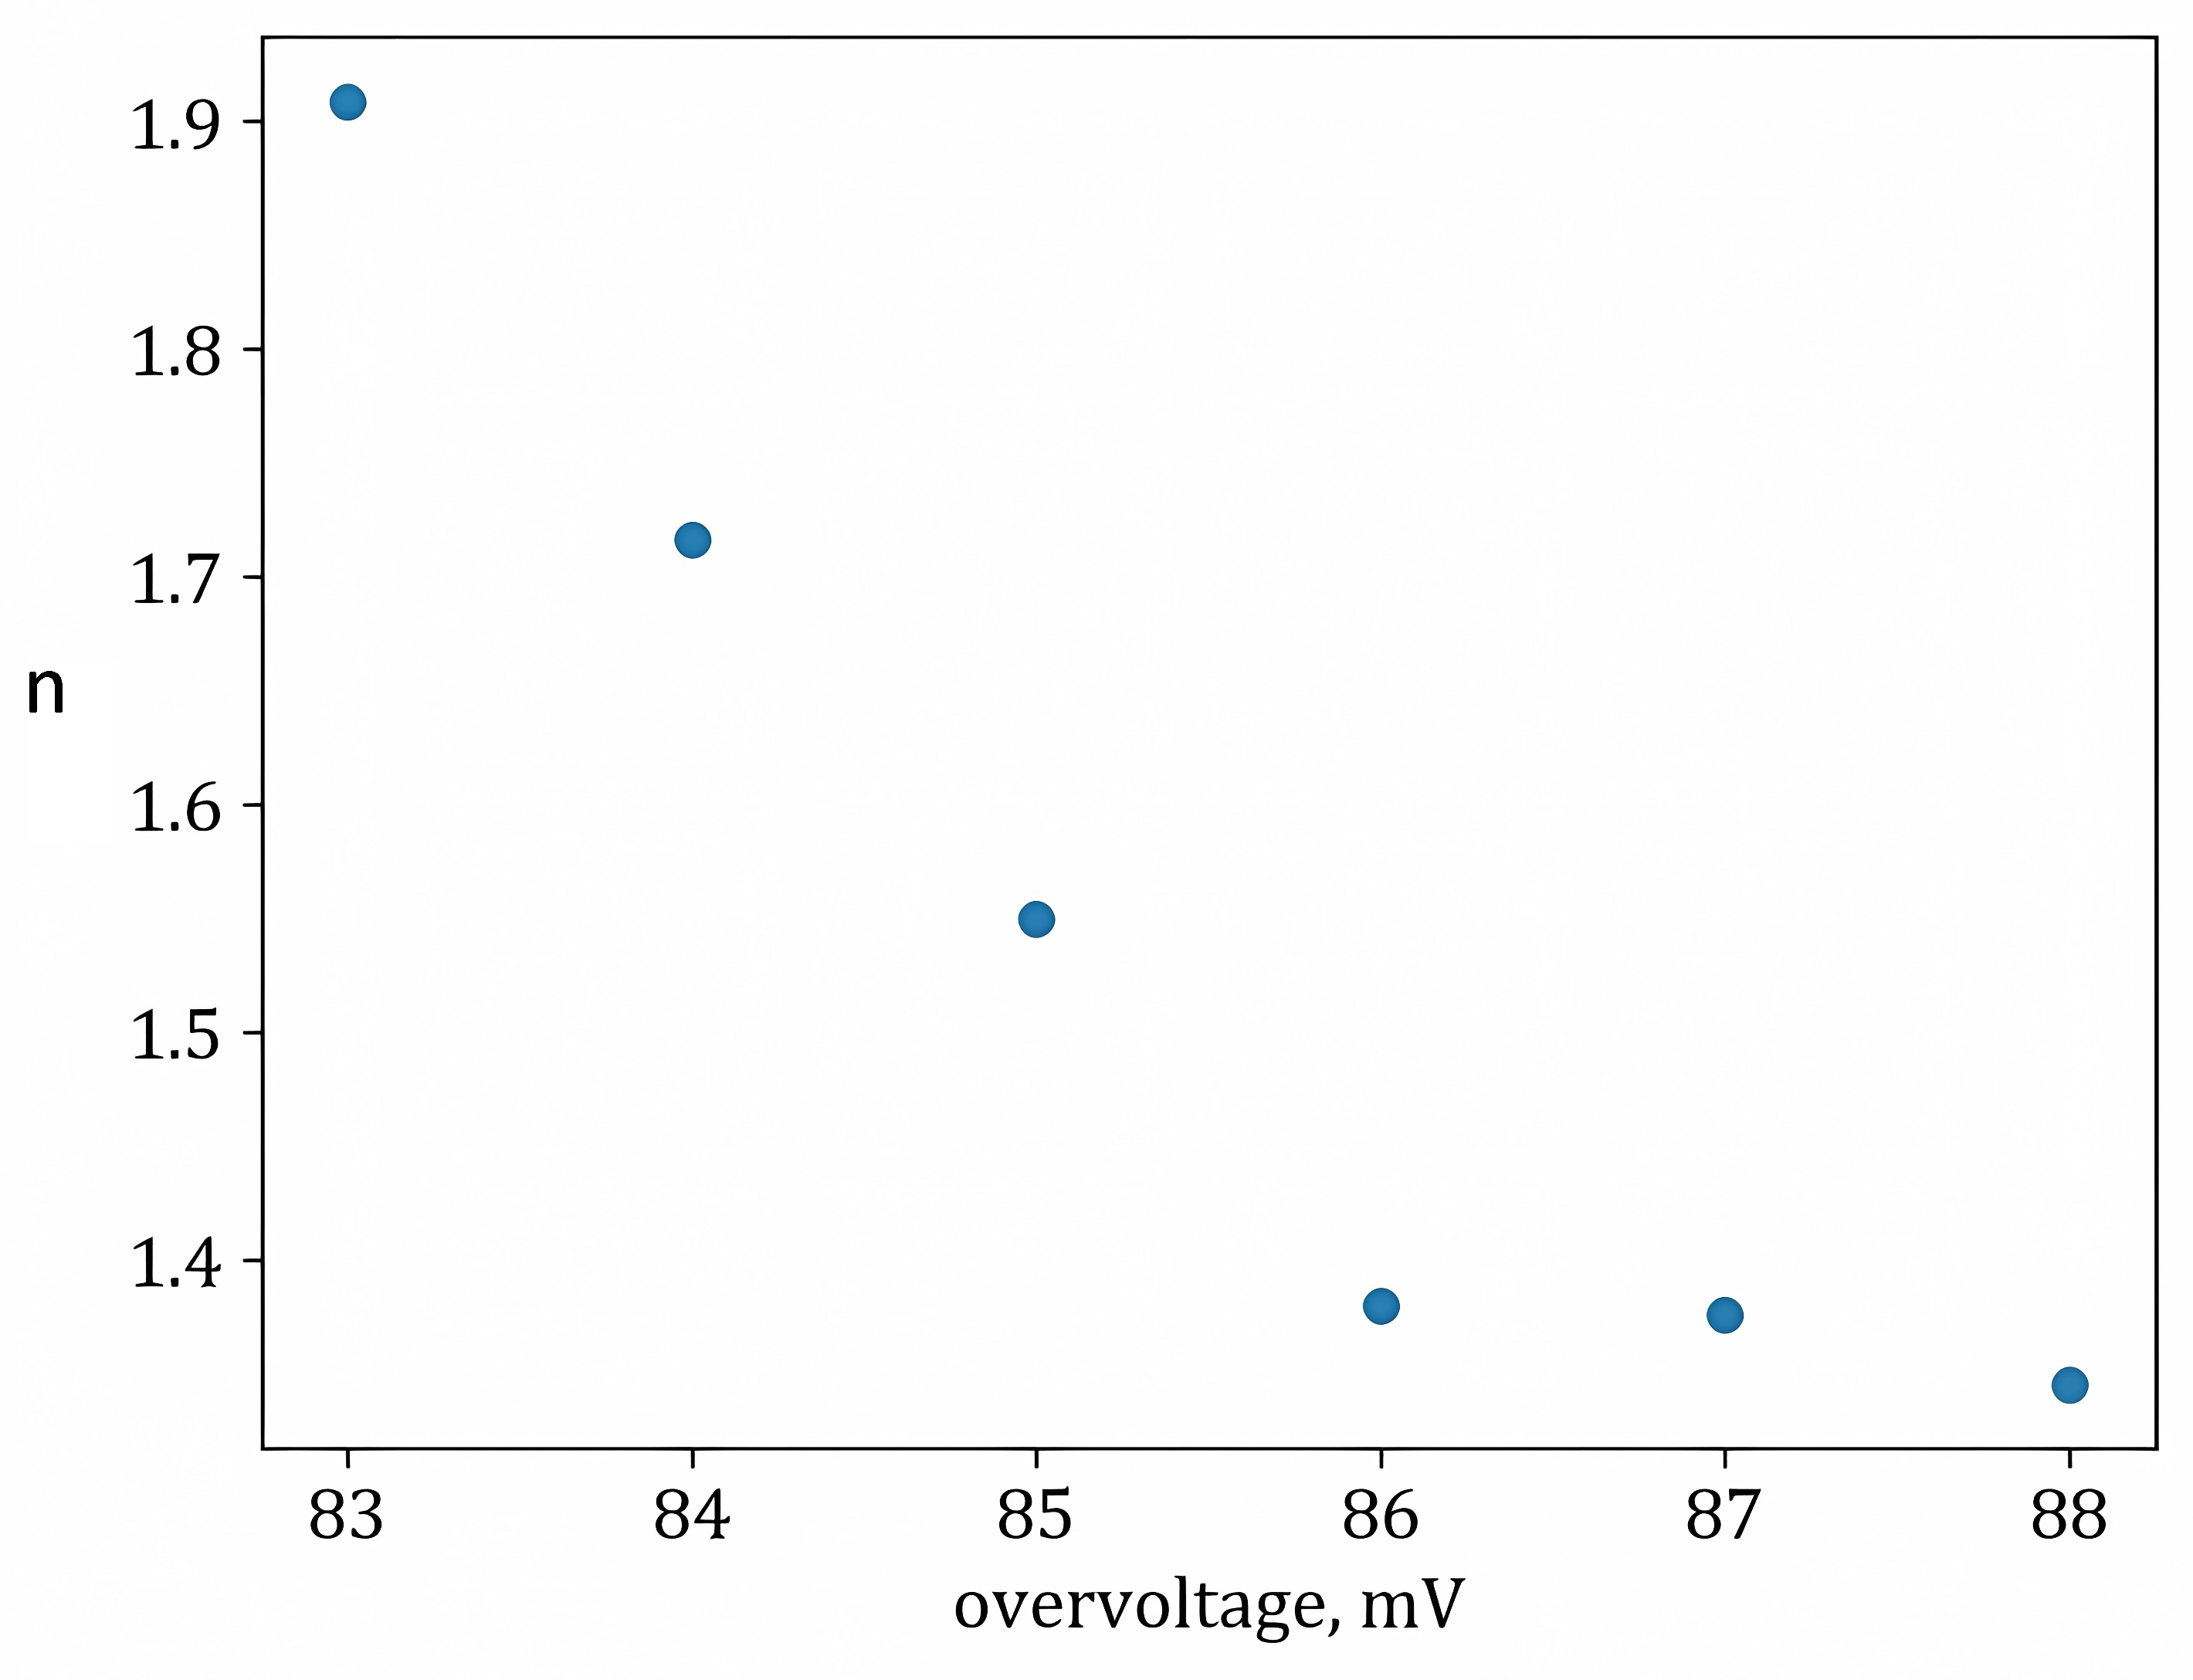
\includegraphics[width=0.48\textwidth]{ivan_markov_graphs/fig6_d_jmakn.png}}
    \caption{Стойности за параметъра $n$ от JMAKn}
\end{figure}
\begin{figure}[H]
    \centering
        \subfloat[Фиг. 5]{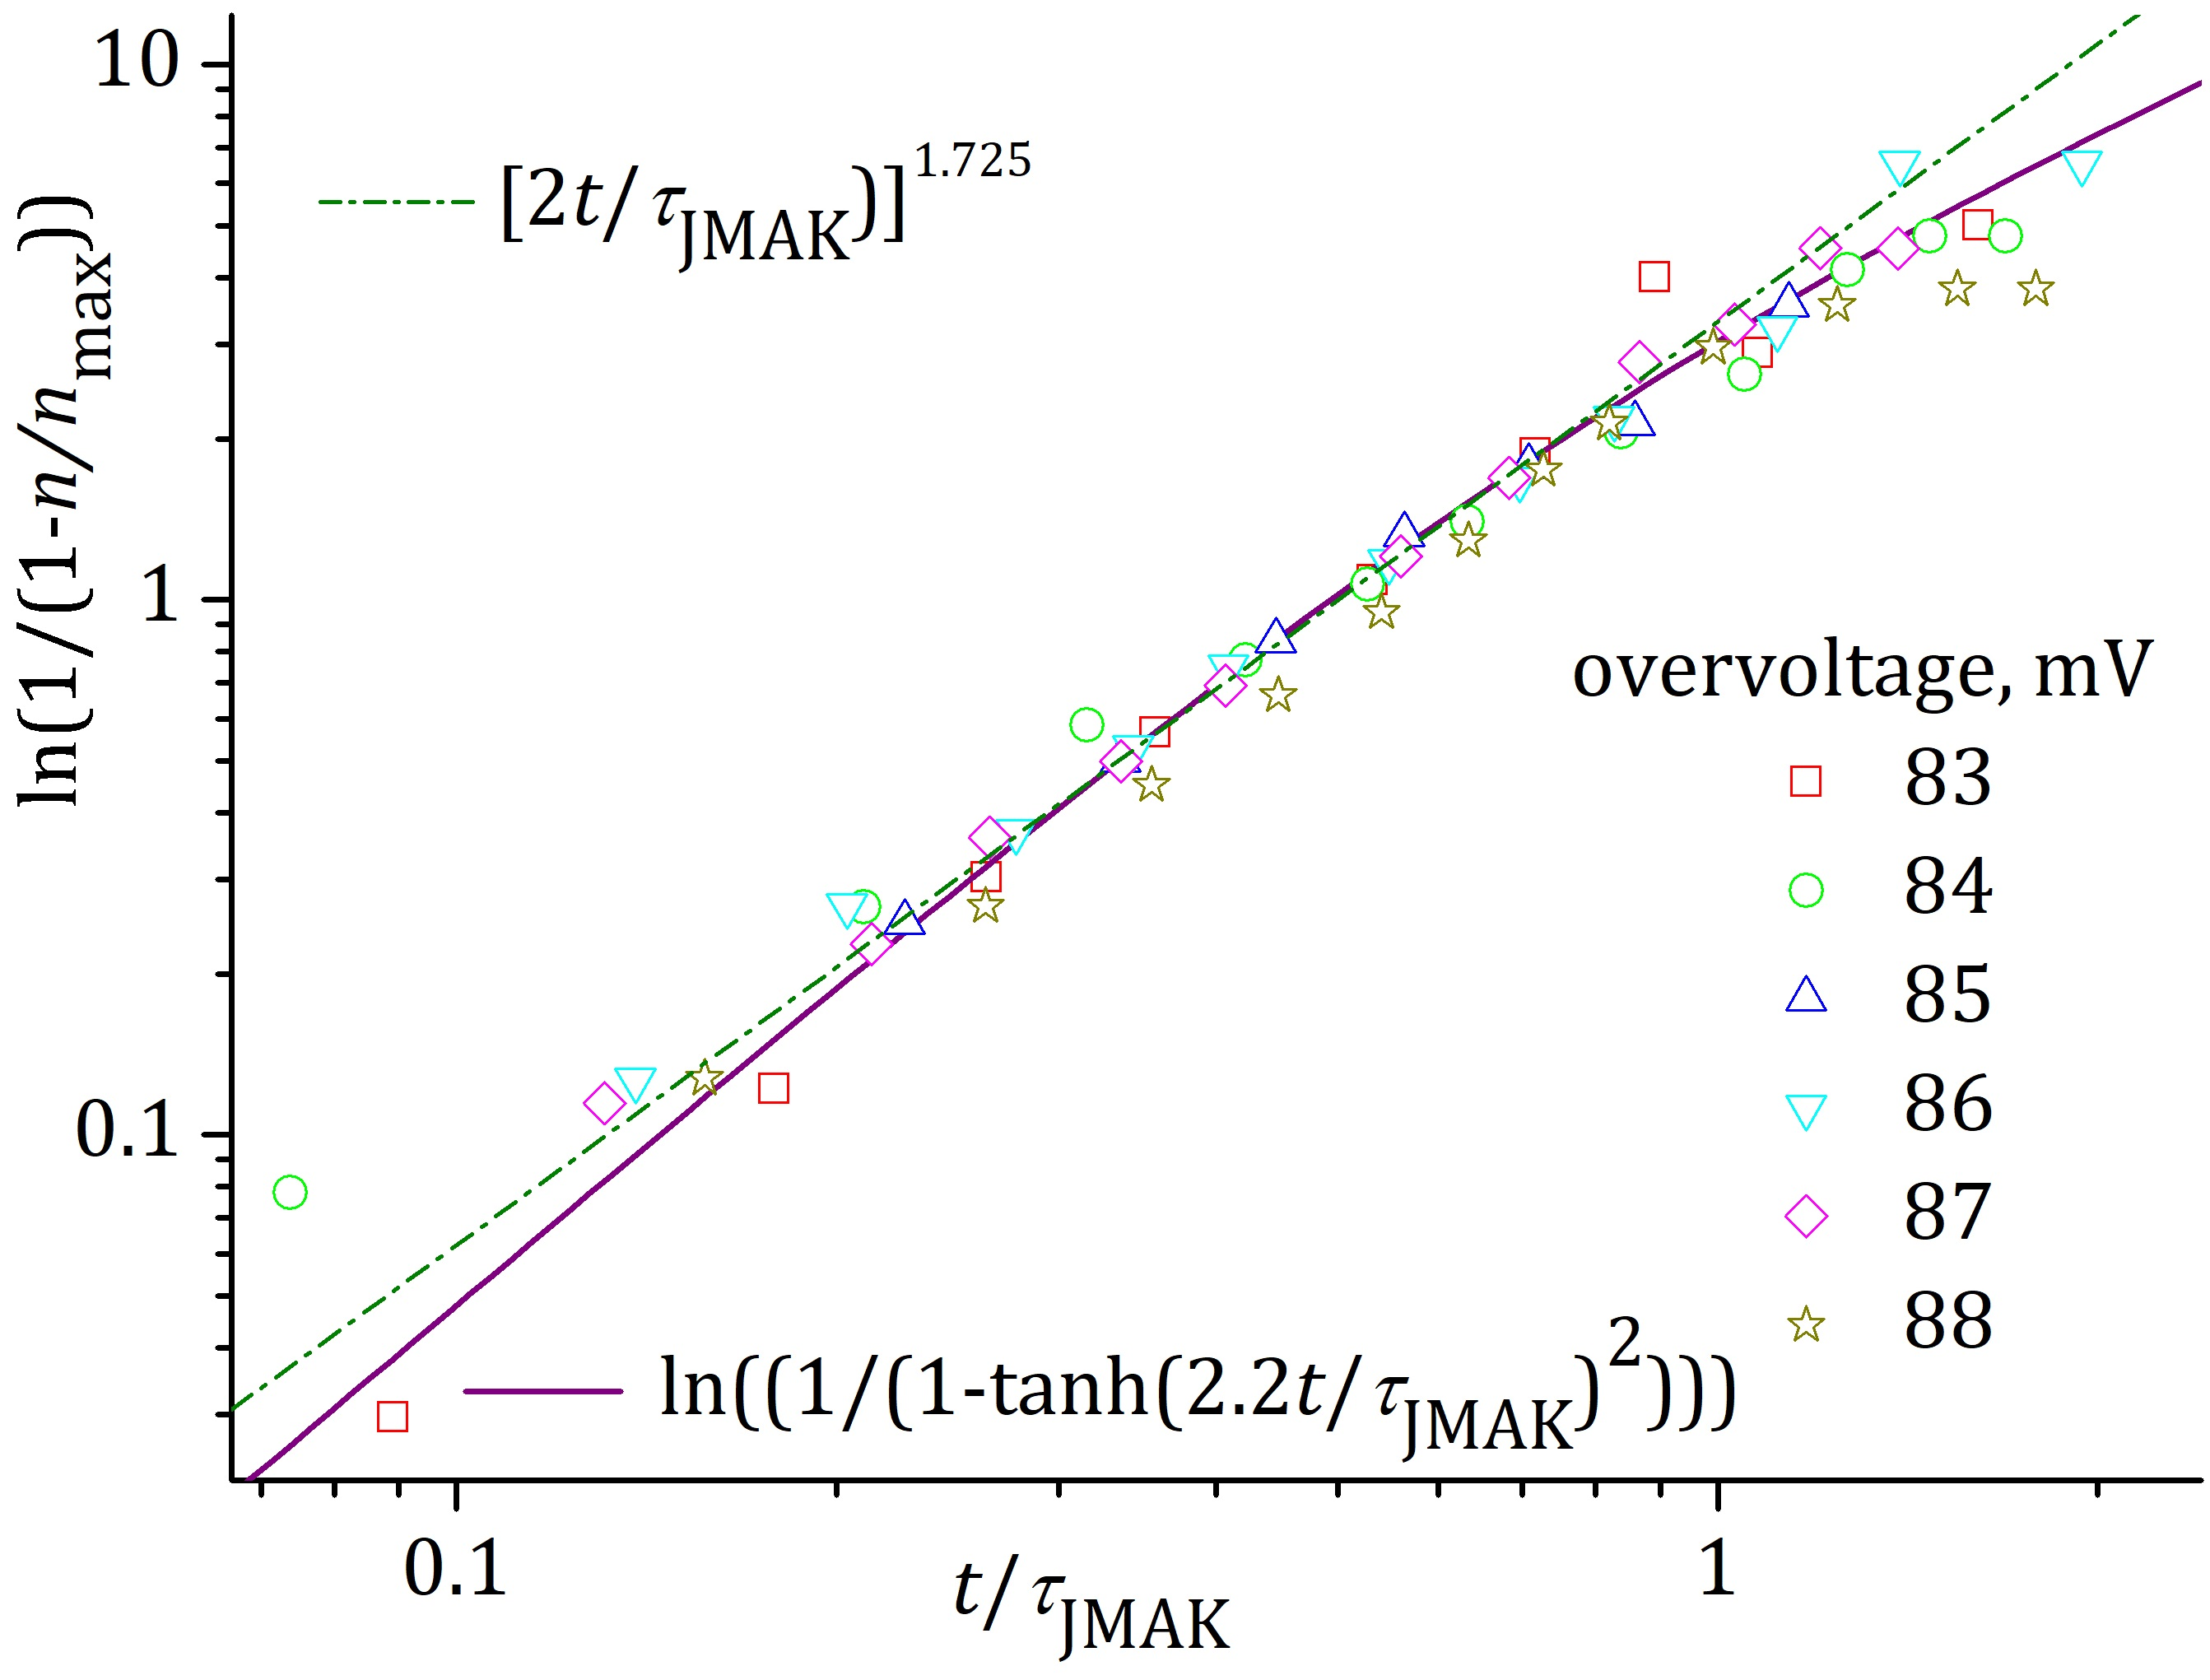
\includegraphics[width=0.48\textwidth]{ivan_markov_graphs/Fig5-jmak_rescaled_inAvramiCoordinates.jpg}}
        \subfloat[Фиг. 6]{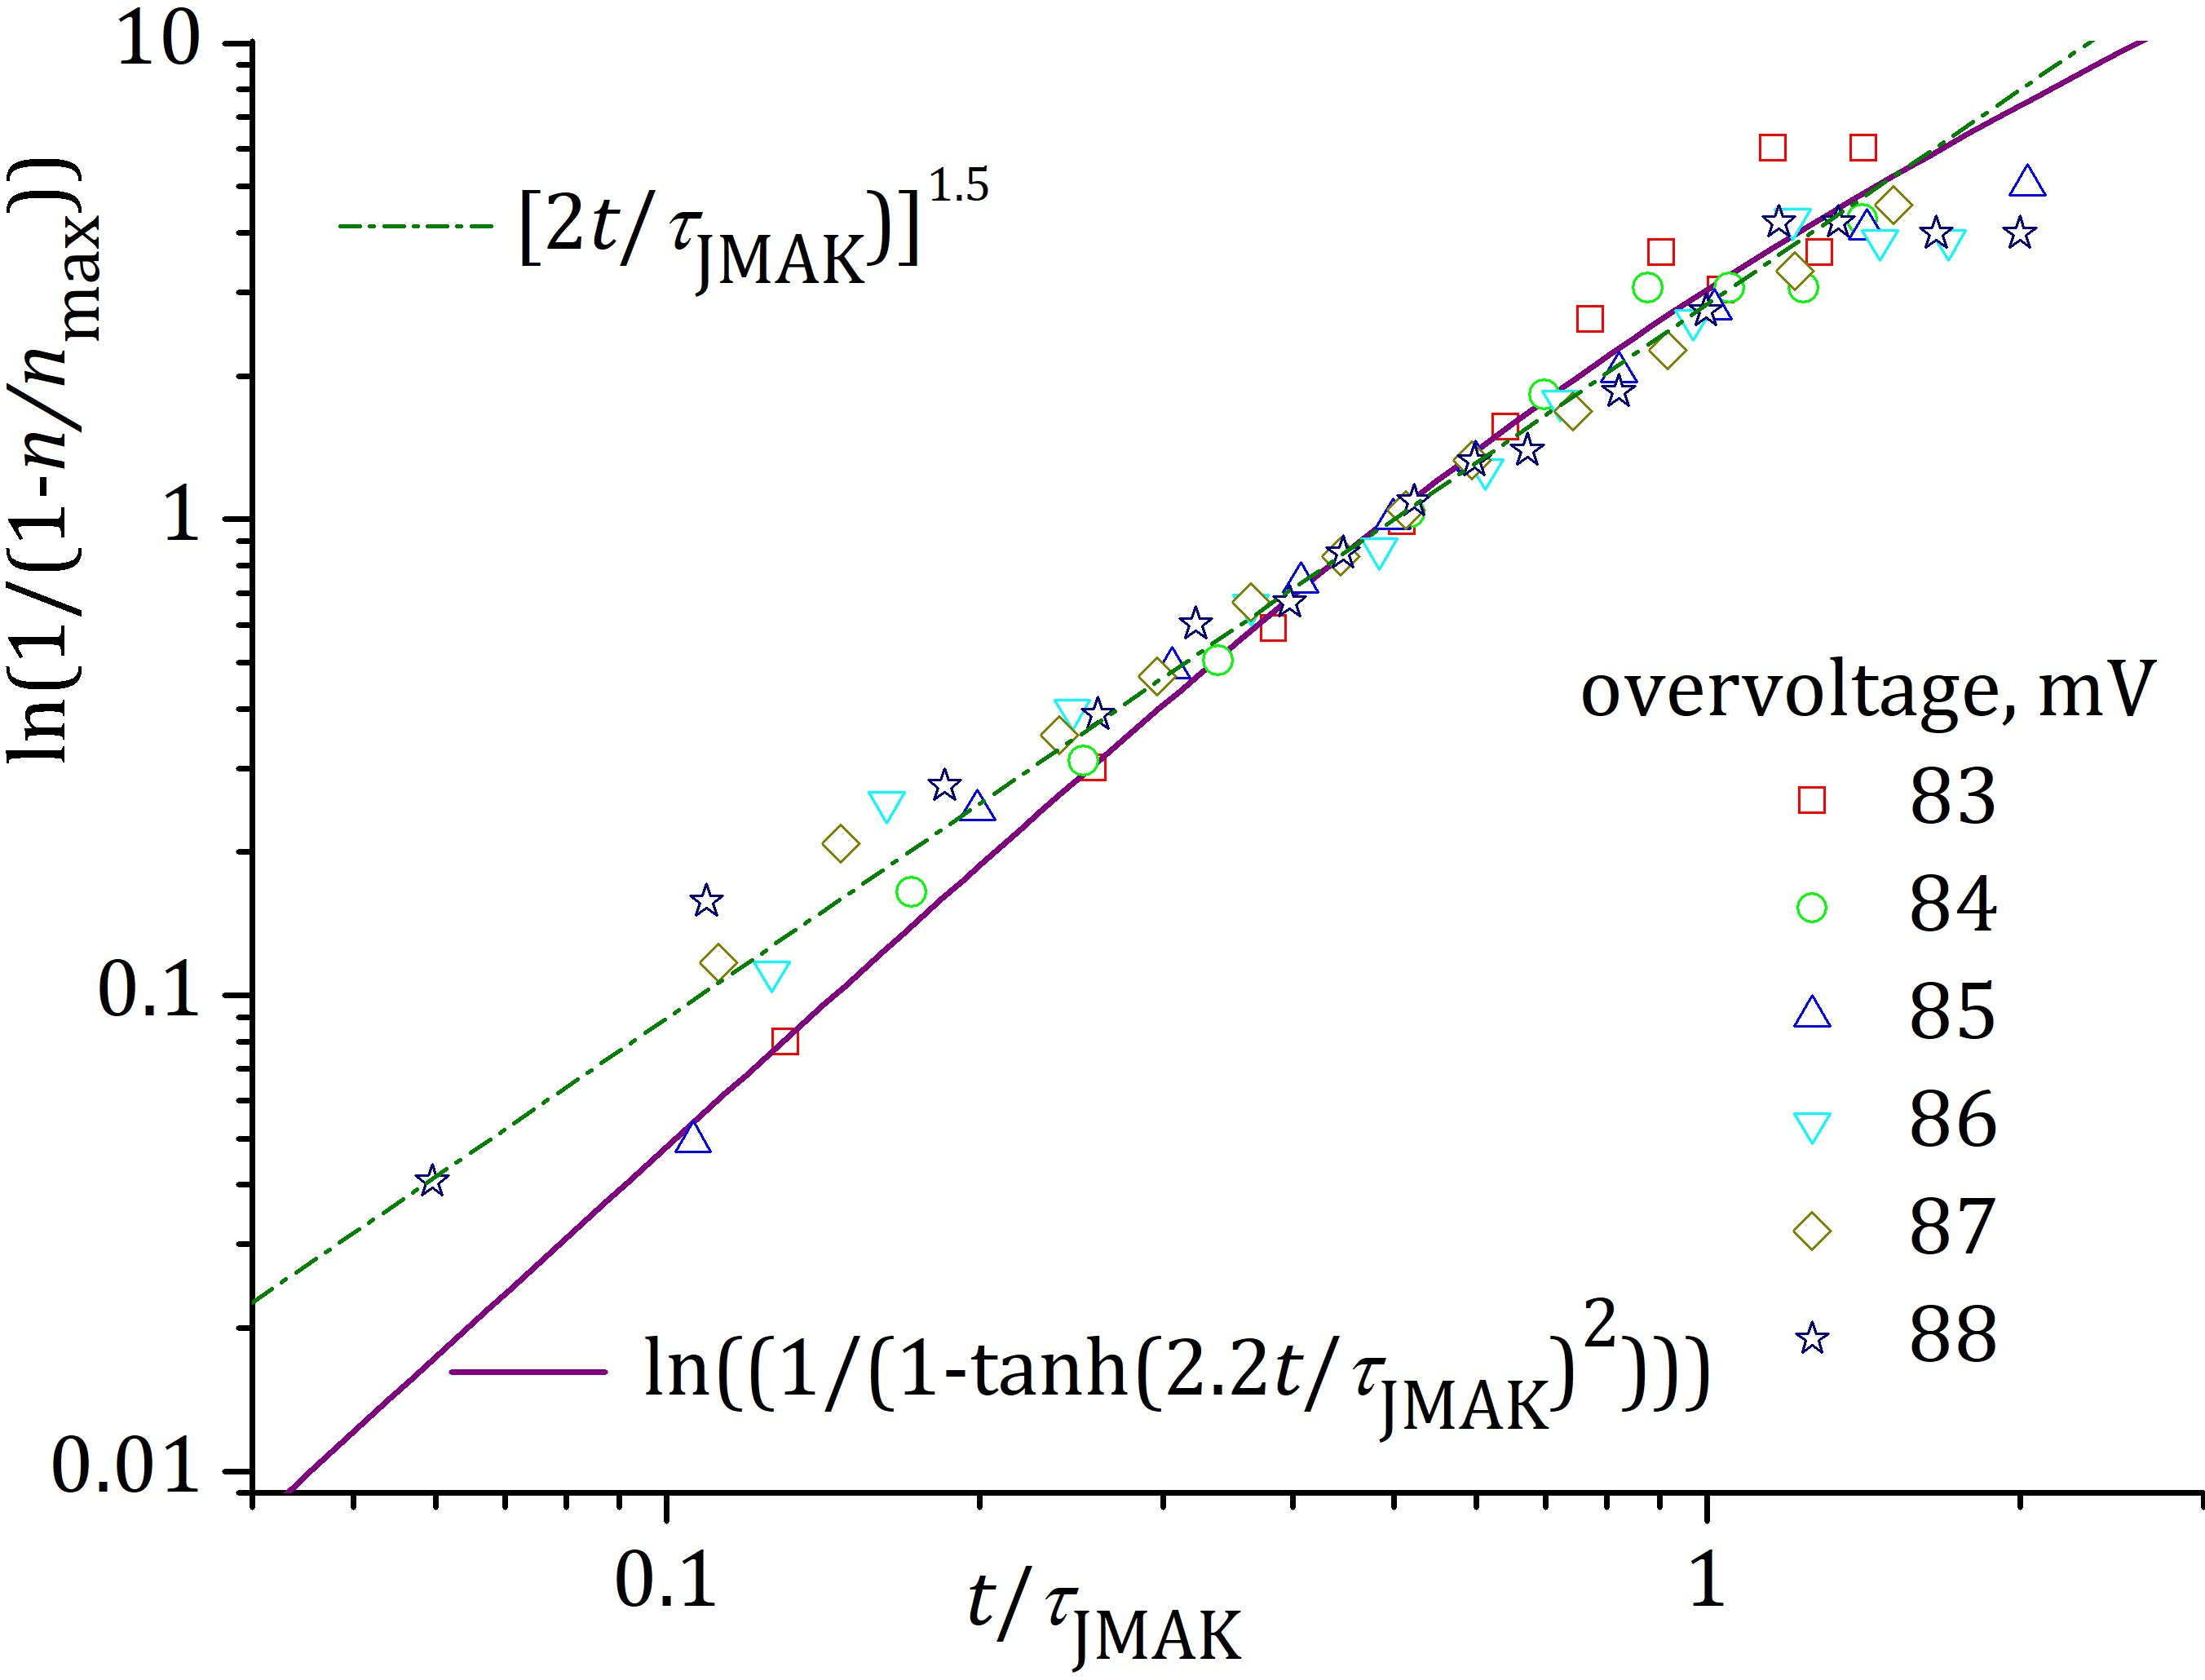
\includegraphics[width=0.48\textwidth]{ivan_markov_graphs/Fig6-jmak_rescaled_inAvramiCoordinates.jpg}}
    \caption{Рескалирани данни от JMAKn за различни свръхпотенциали в Аврами координати}
    \label{fig:jmakn_ivan_markov_avrami_plot}
\end{figure}
\autoref{fig:jmakn_ivan_markov_avrami_plot} представя много ясно основните слабости на JMAKn - несъответствието на модела на поведението на данните в Аврами координати за малки $\alpha$ и завоят за $\alpha \rightarrow 1$ спрямо $n$.

Липсата на универсална крива може да бъде пропуснато тук заради близките стойности на $n$, т.е. получените резултати за този параметър грубо да бъдат закръглени, но това ще доведе до съответно понижаване на $R^2$, тъй като моделът е нелинеен и чувствителен към промените на $n$.
\subsubsection{Модел \texorpdfstring{$\alpha_{21}$}{α21}}
\begin{figure}[H]
    \centering
        \subfloat[Фиг. 5]{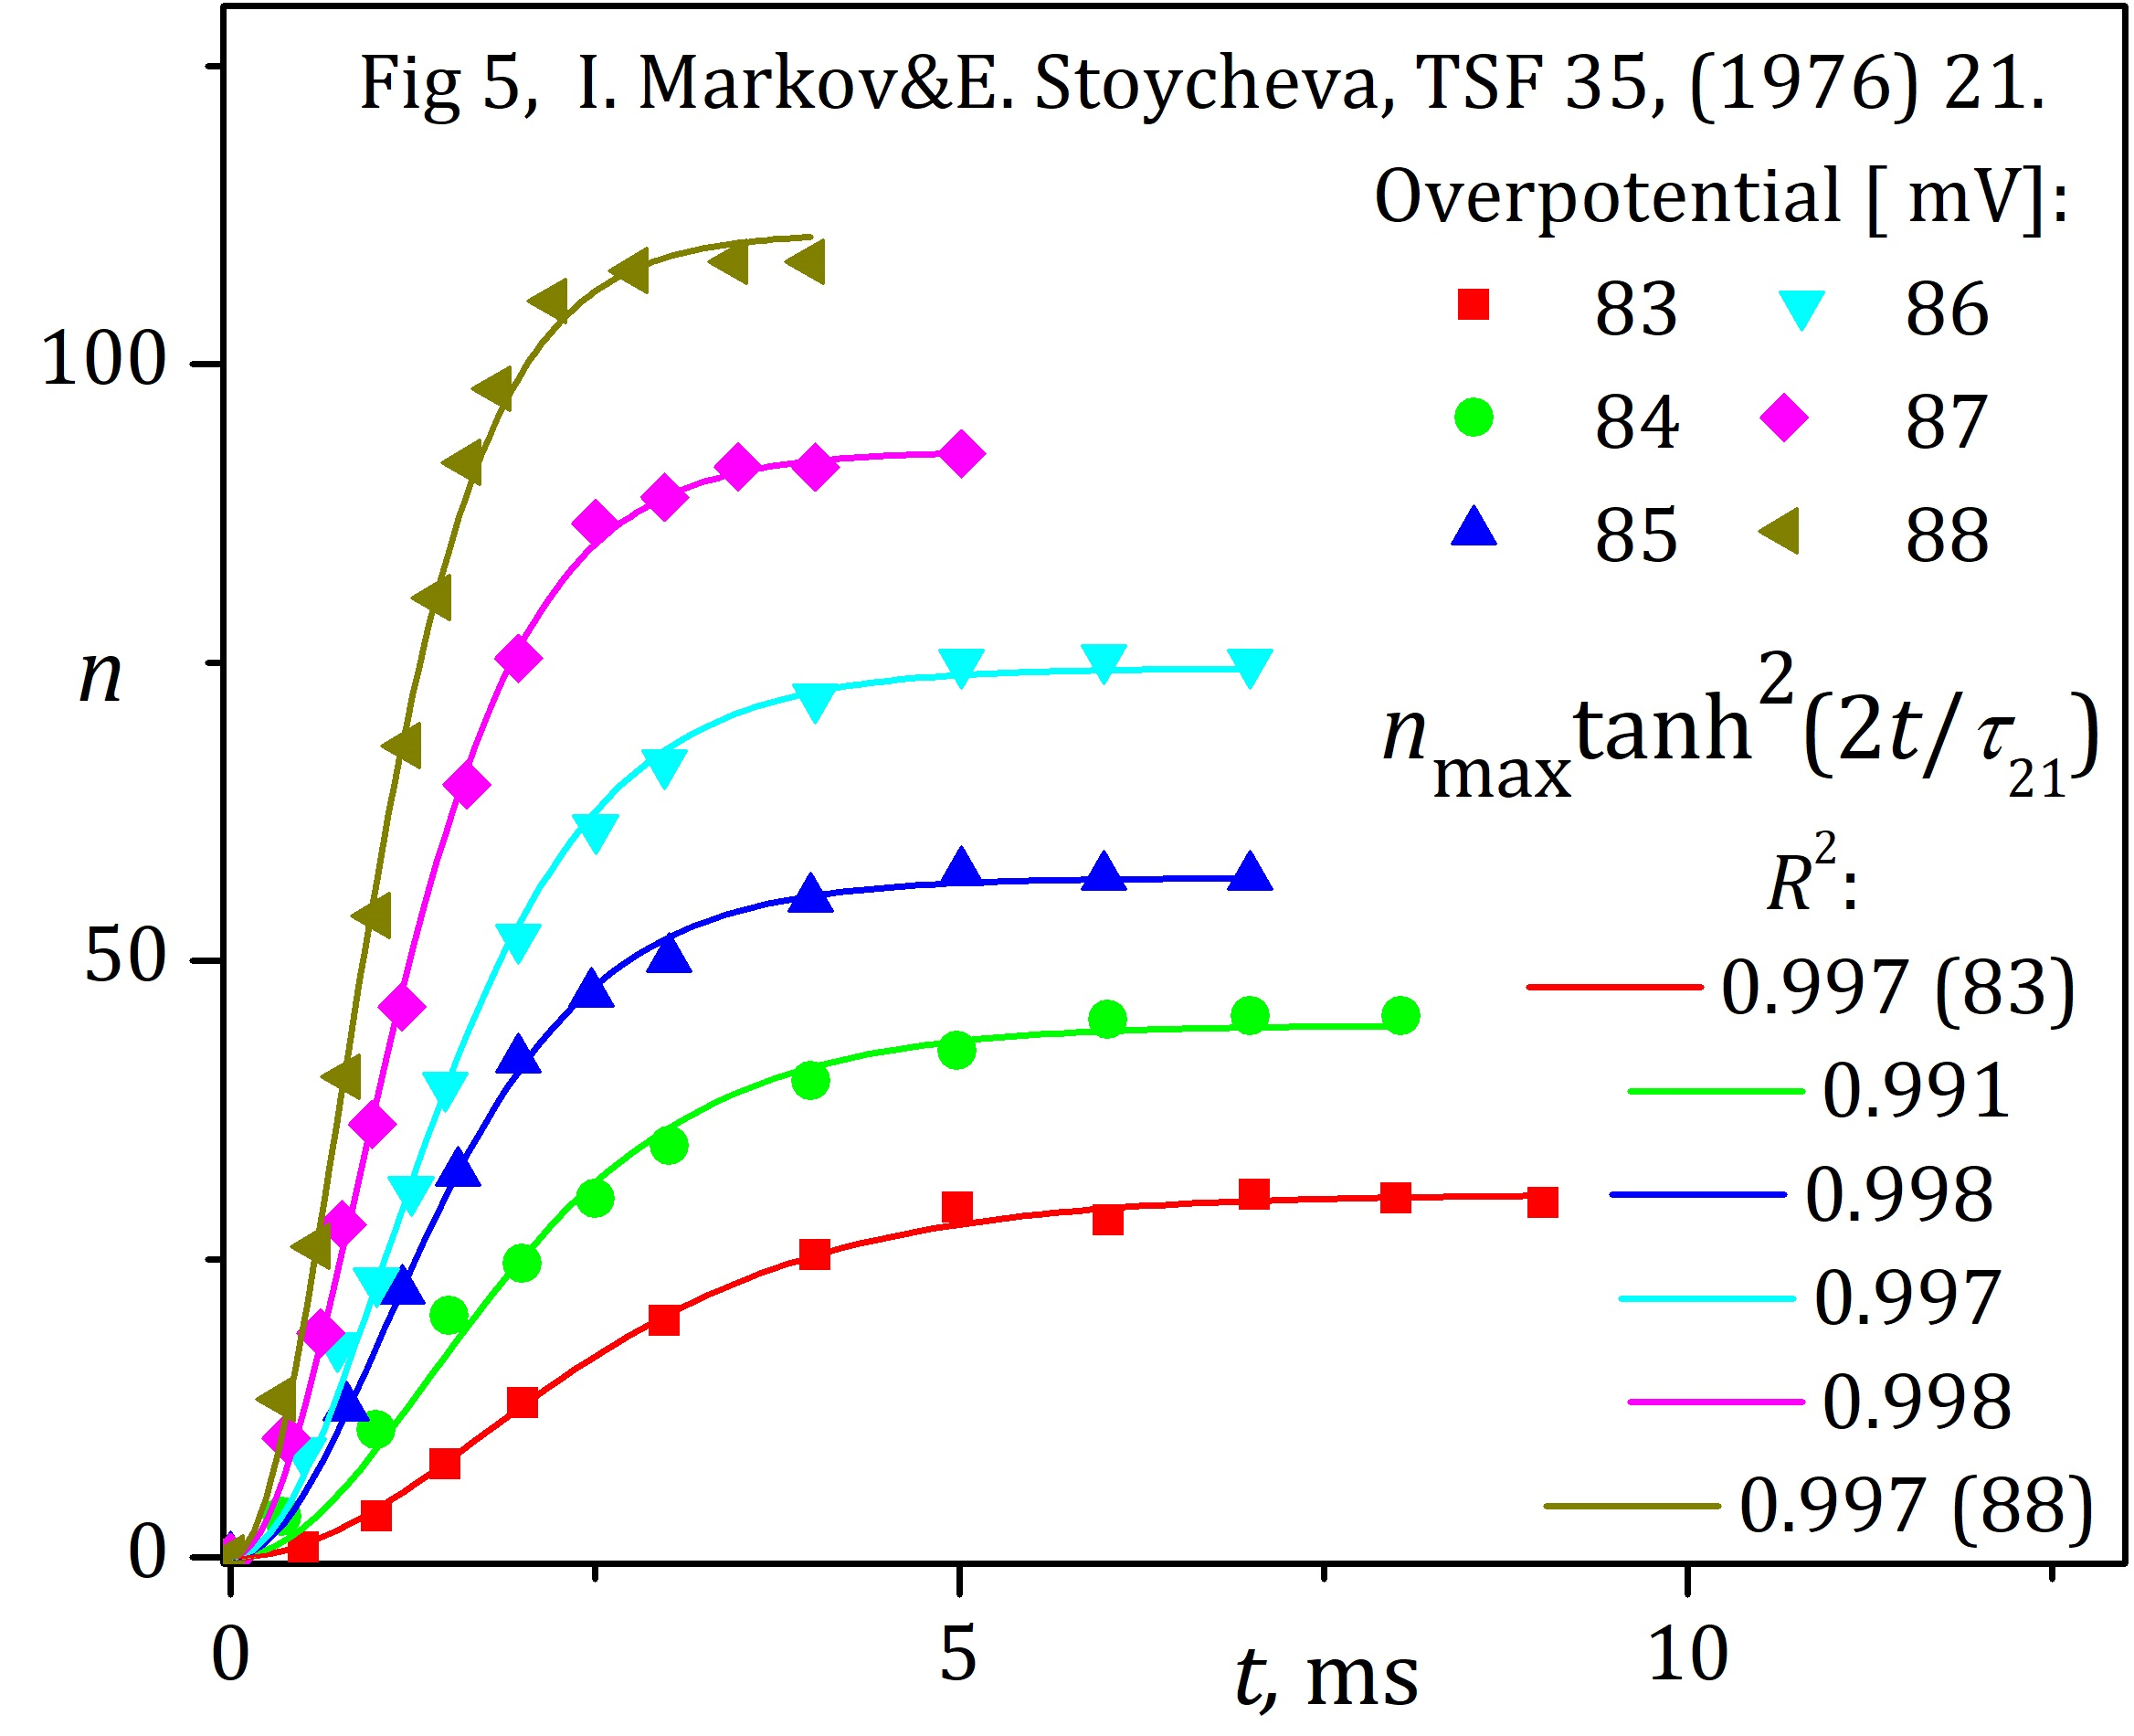
\includegraphics[width=0.48\textwidth]{ivan_markov_graphs/Fig5-alfa21-direct.jpg}}
        \subfloat[Фиг. 6]{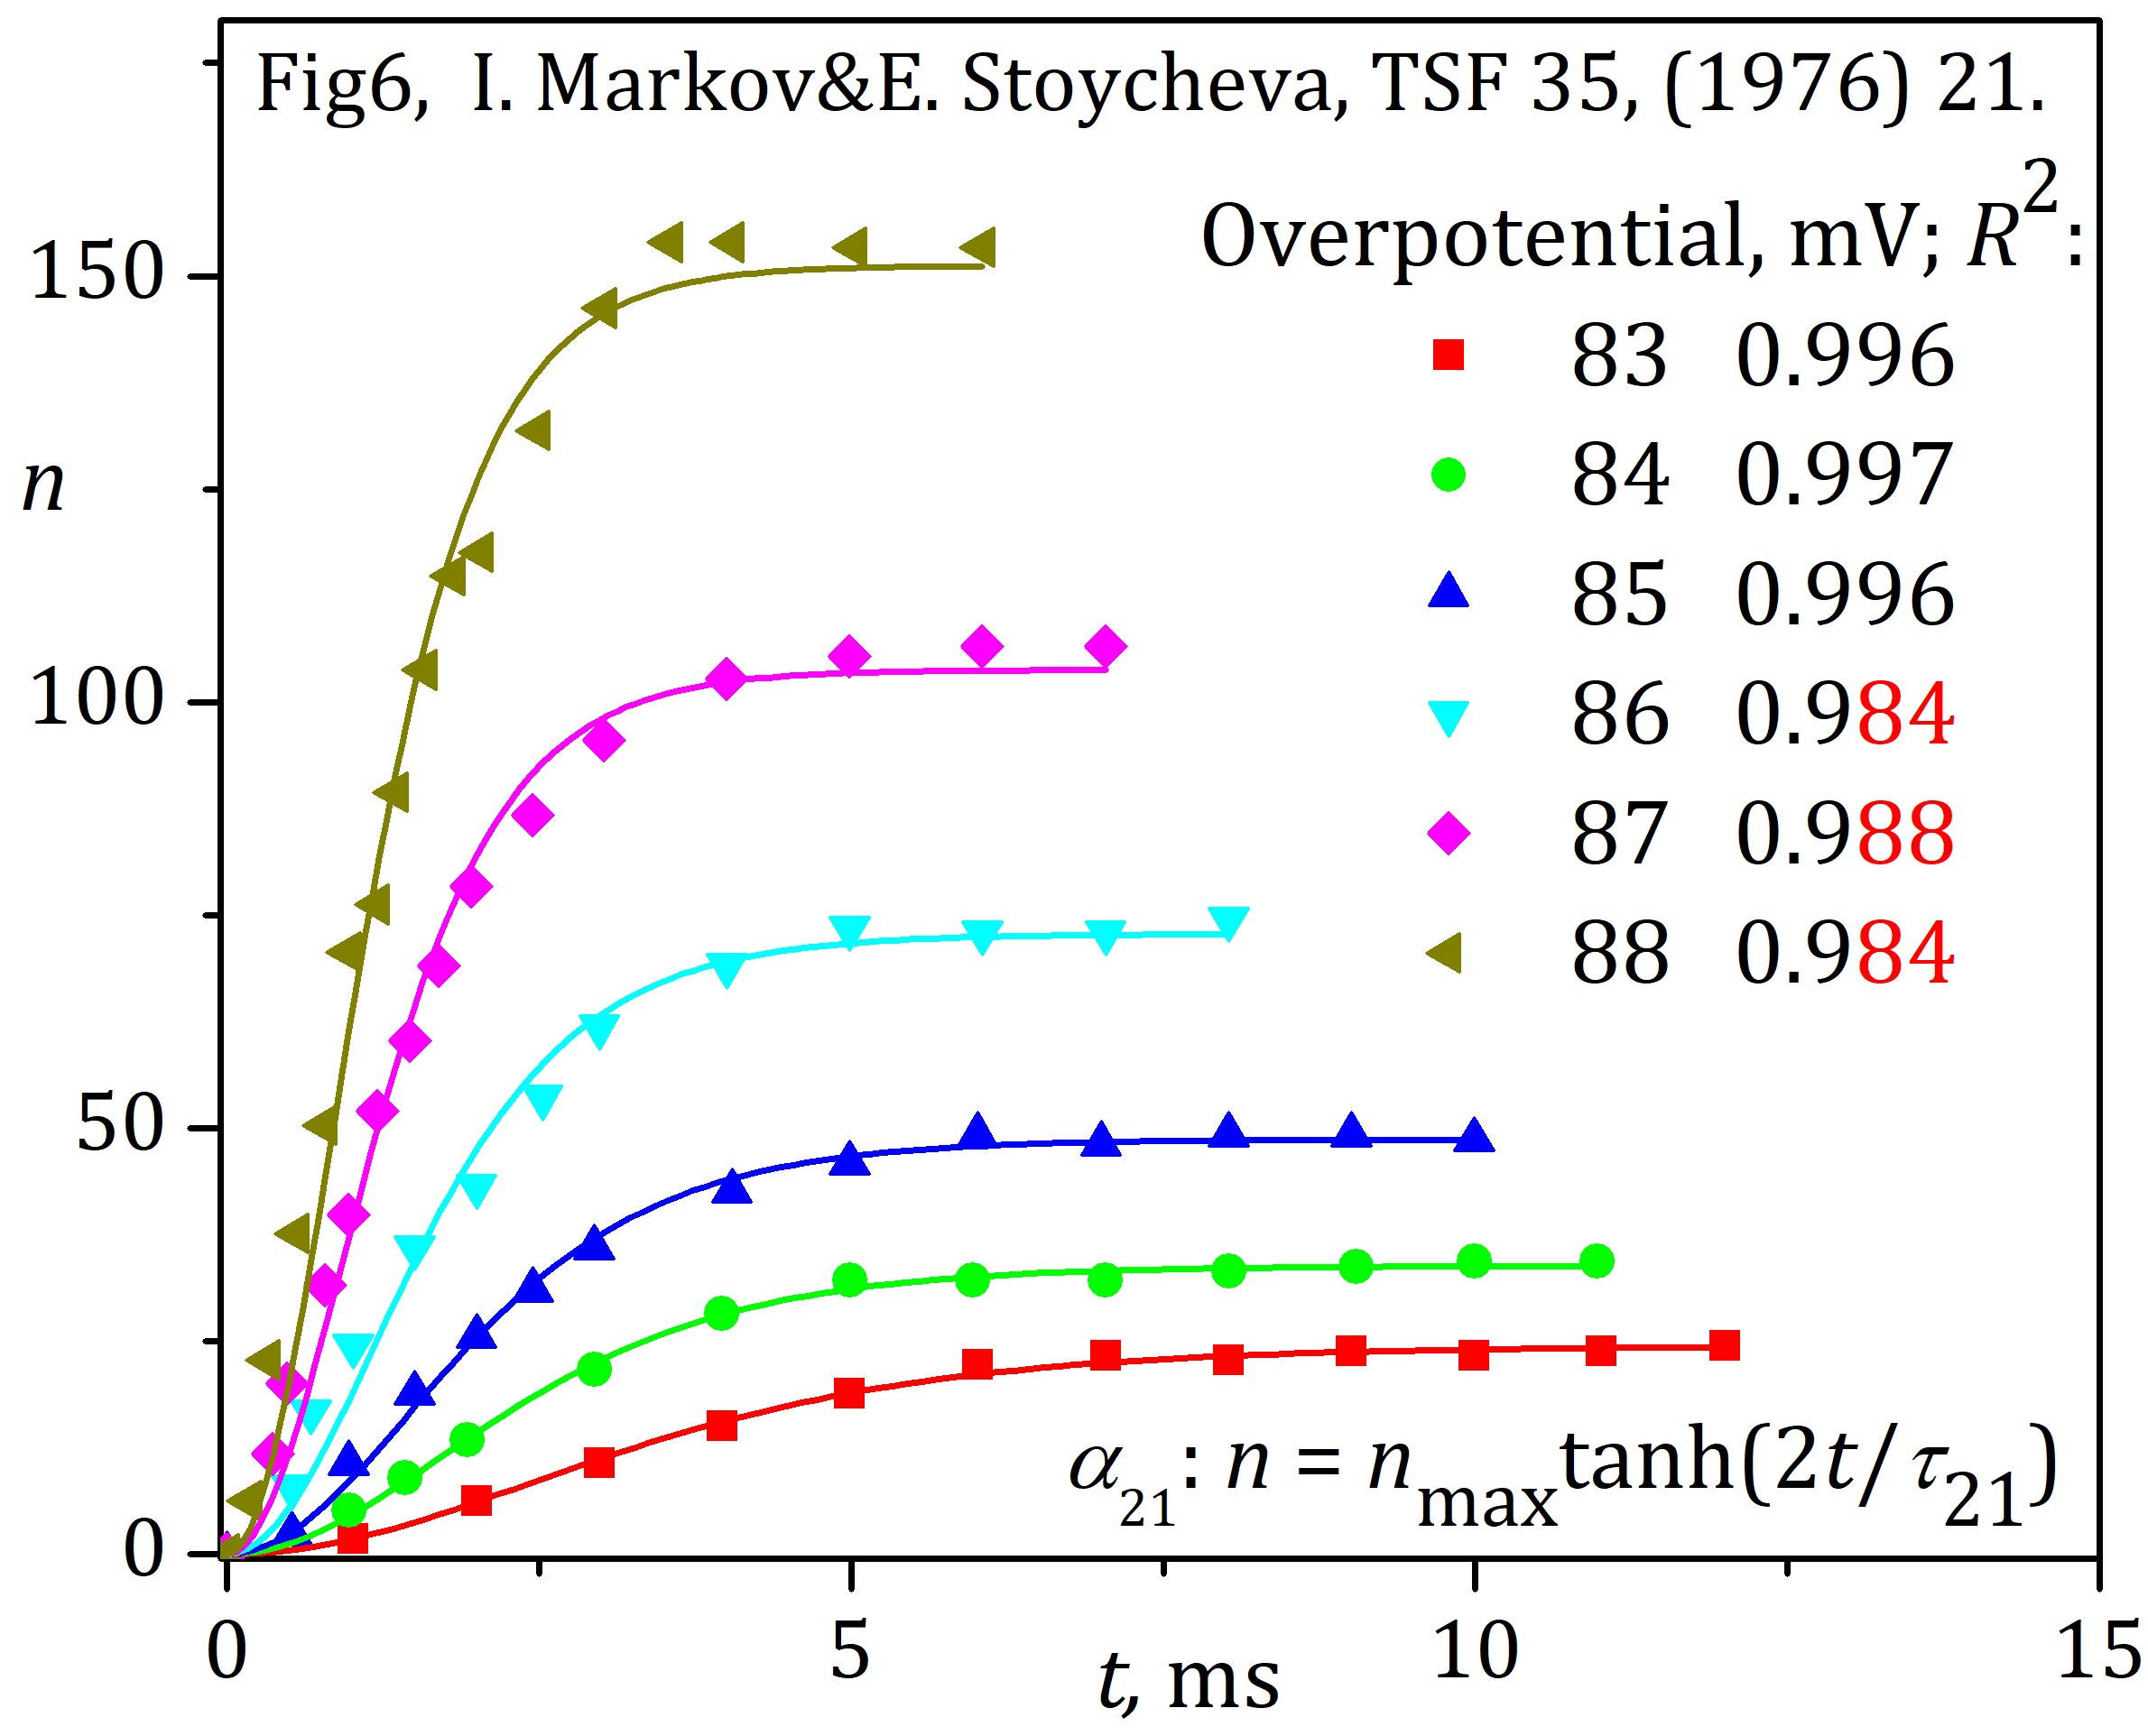
\includegraphics[width=0.48\textwidth]{ivan_markov_graphs/Fig6_alfa21-direct.jpg}}
    \caption{Данни от \cite{Markov1976} и съответните криви за $\alpha_{21}$ и съответни стойности за $R^2$}
\end{figure}

Тъй като имаме единствен параметър ($\tau_{21}$) освен $N_{max}$, можем да представим всички данни на универсална крива. Това е и основно достойнство на изведения от нас модел.

\begin{figure}[H]
    \centering
        \subfloat[Фиг. 5]{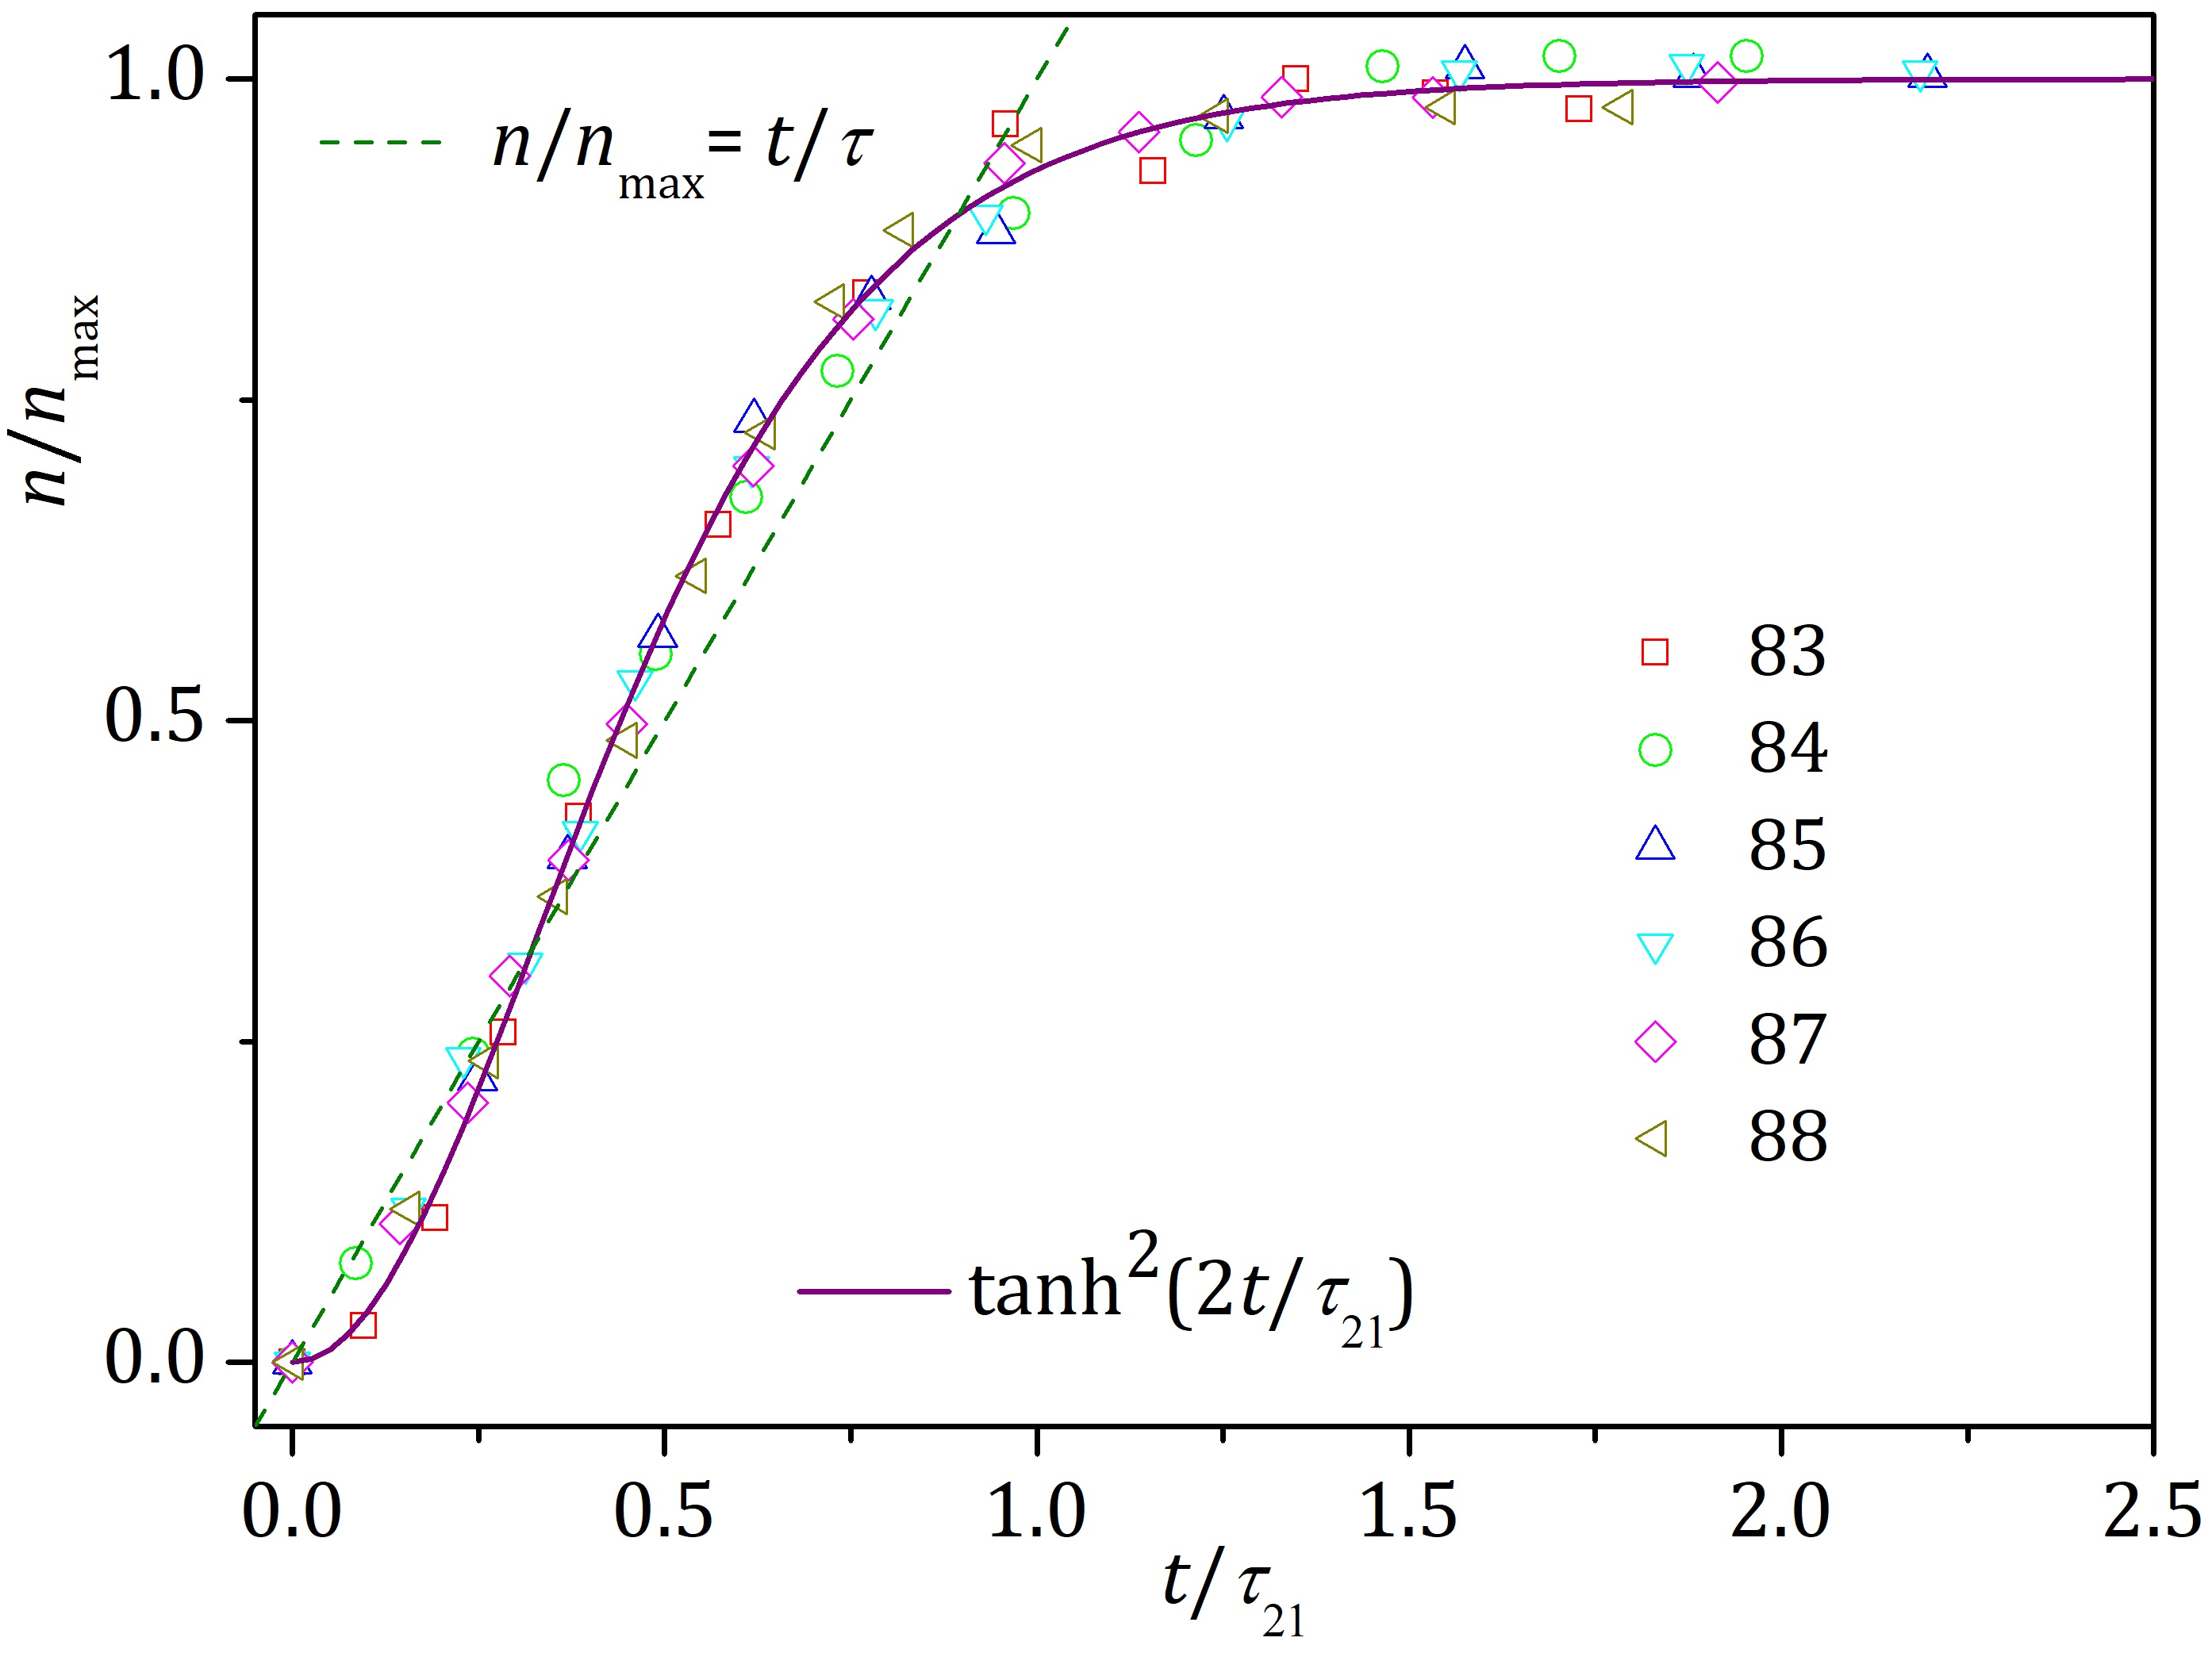
\includegraphics[width=0.48\textwidth]{ivan_markov_graphs/Fig5-alfa21_rescaled.jpg}}
        \subfloat[Фиг. 6]{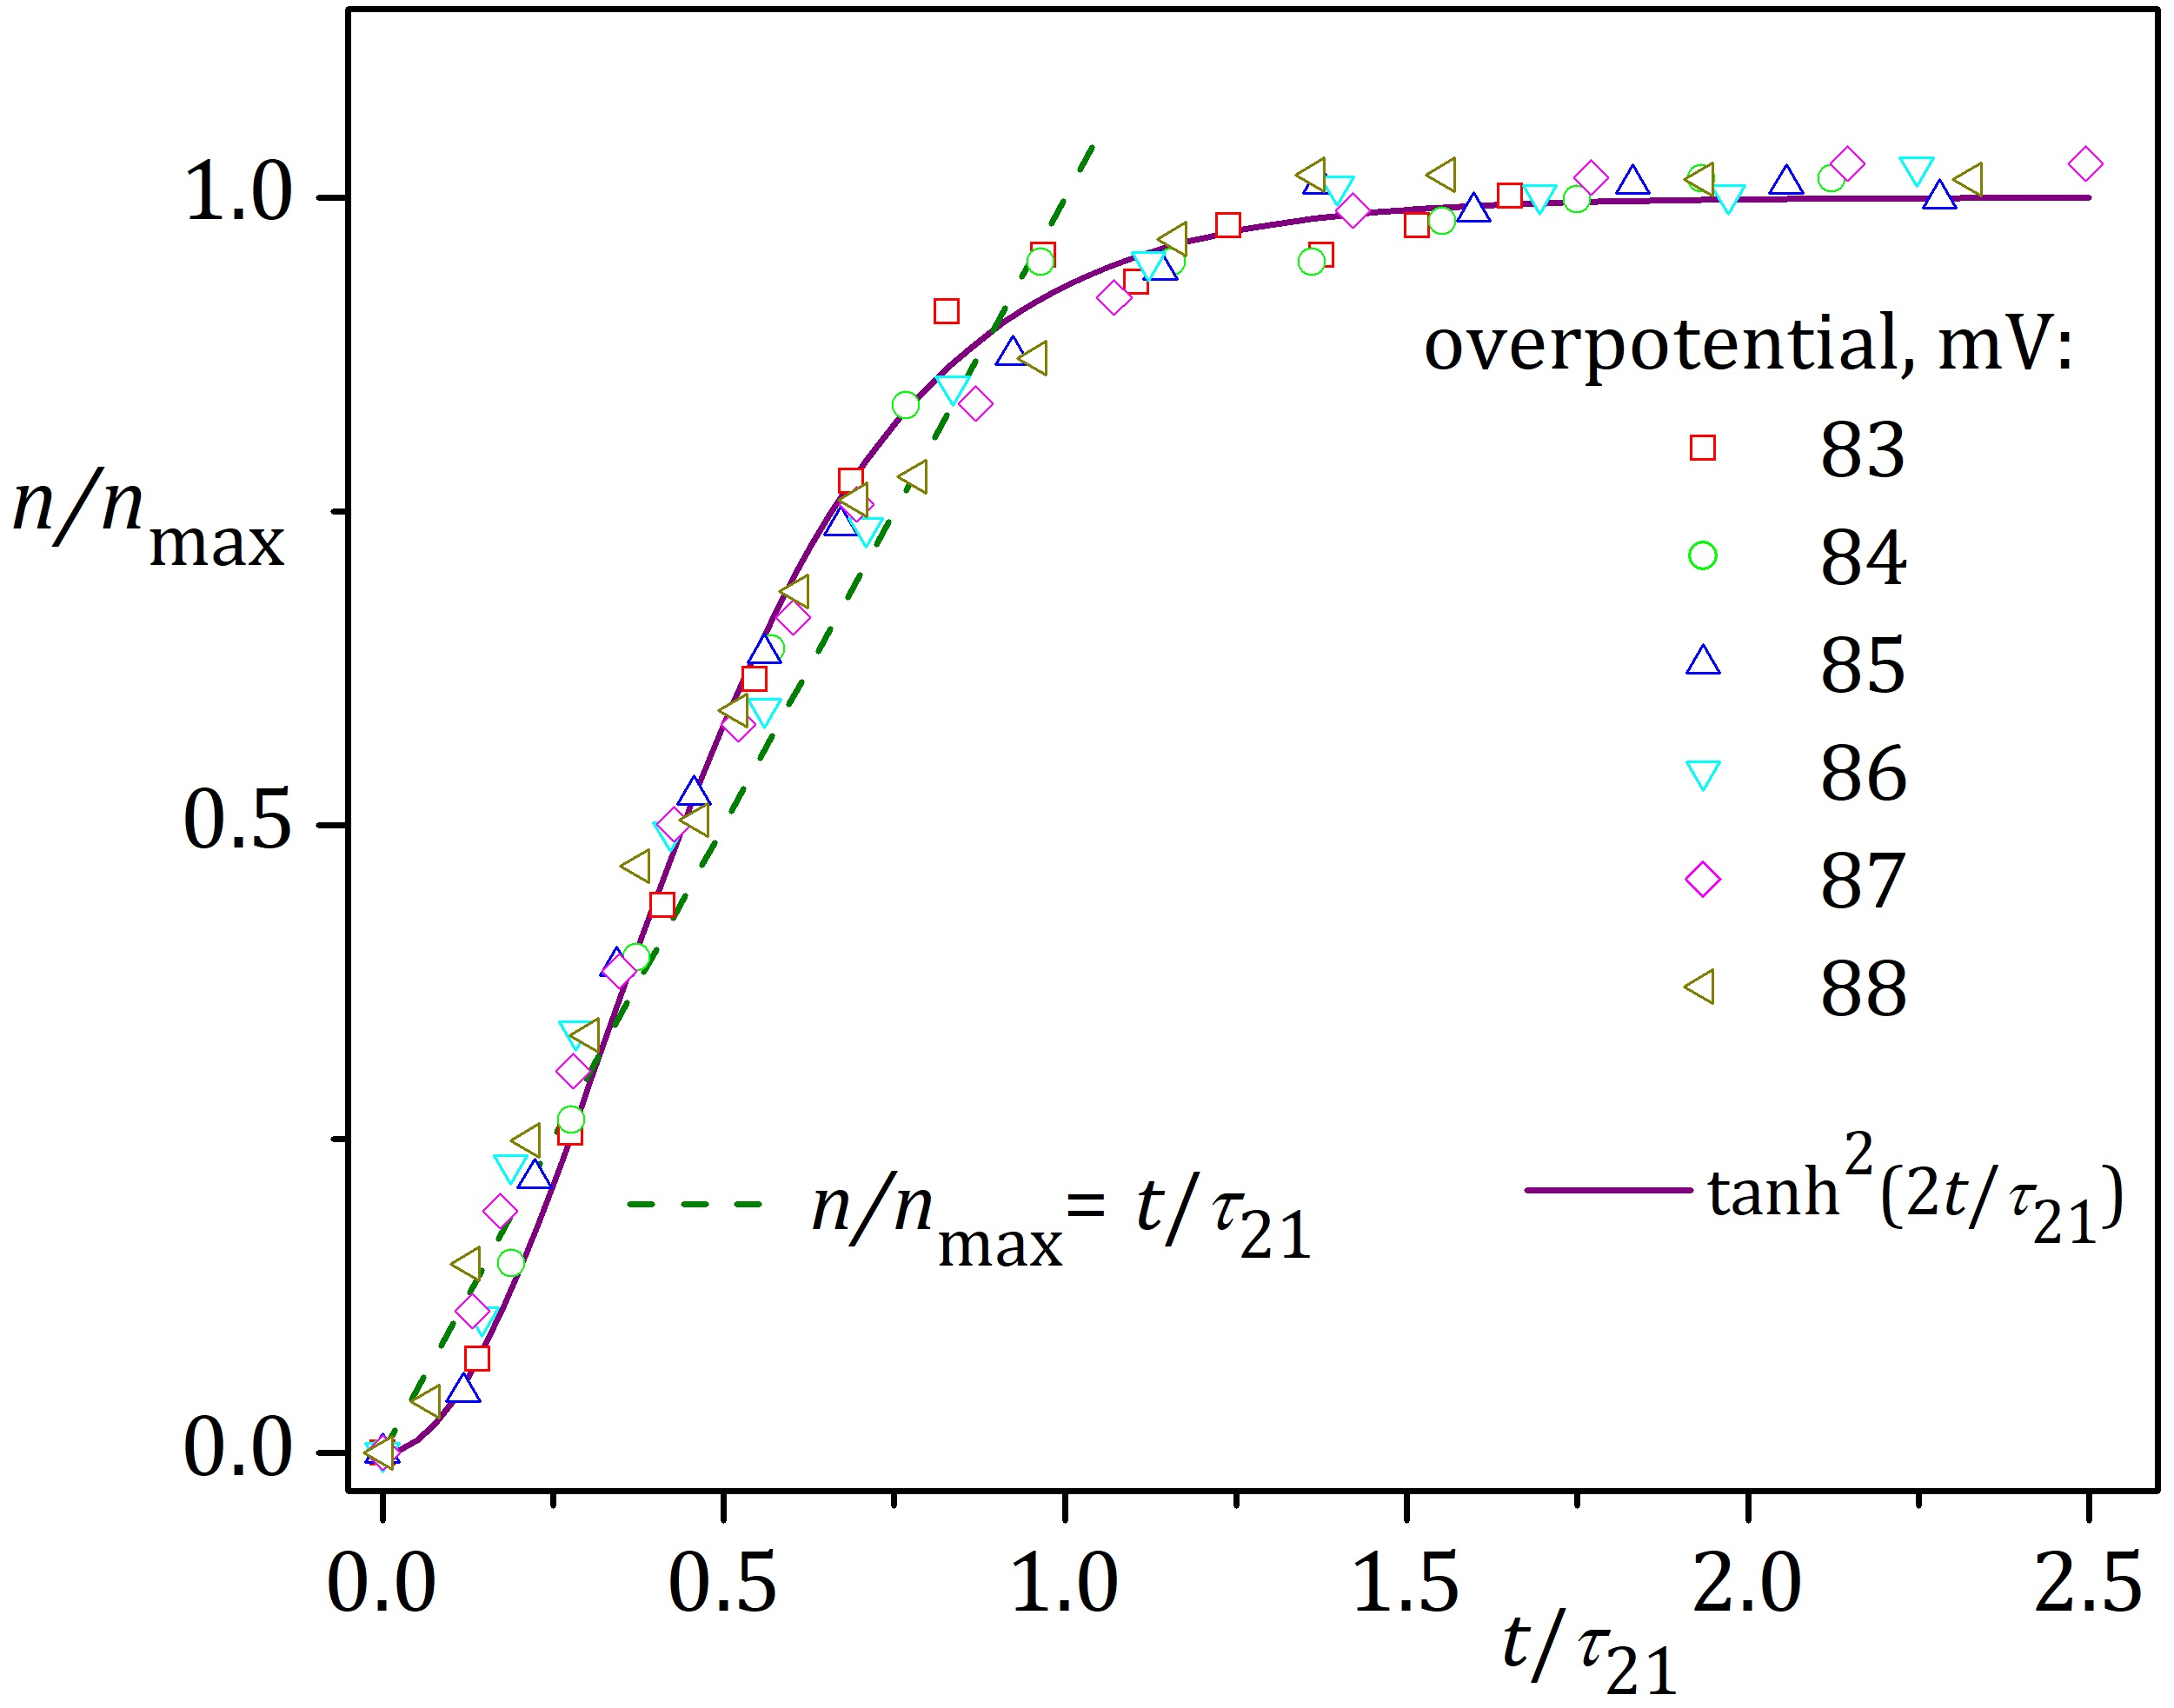
\includegraphics[width=0.48\textwidth]{ivan_markov_graphs/Fig6_alfa21_rescaled.jpg}}
    \caption{Рескалирани данни от \cite{Markov1976} и универсалната крива за $\alpha_{21}$}
    \label{fig:alfa21_ivan_markov_master_curve}
\end{figure}
\autoref{fig:alfa21_ivan_markov_master_curve} представя апотеоза на нашите разглеждания до тук - от чисто физичните съображения (потвърдени с резултатите за $n$ от JMAKn) избрахме $\aDg$ аналитична крива. За различните експериментални условия определихме $N_{max}$ и $\tau$. Тези параметри използваме след това, за да рескалираме експерименталните данни. Така получаваме универсално поведение, което не може да бъде разкрито с моделите с повече параметри.
\begin{figure}[H]
    \centering
        \subfloat[Фиг. 5\label{subfig:alfa21_params_fig5}]{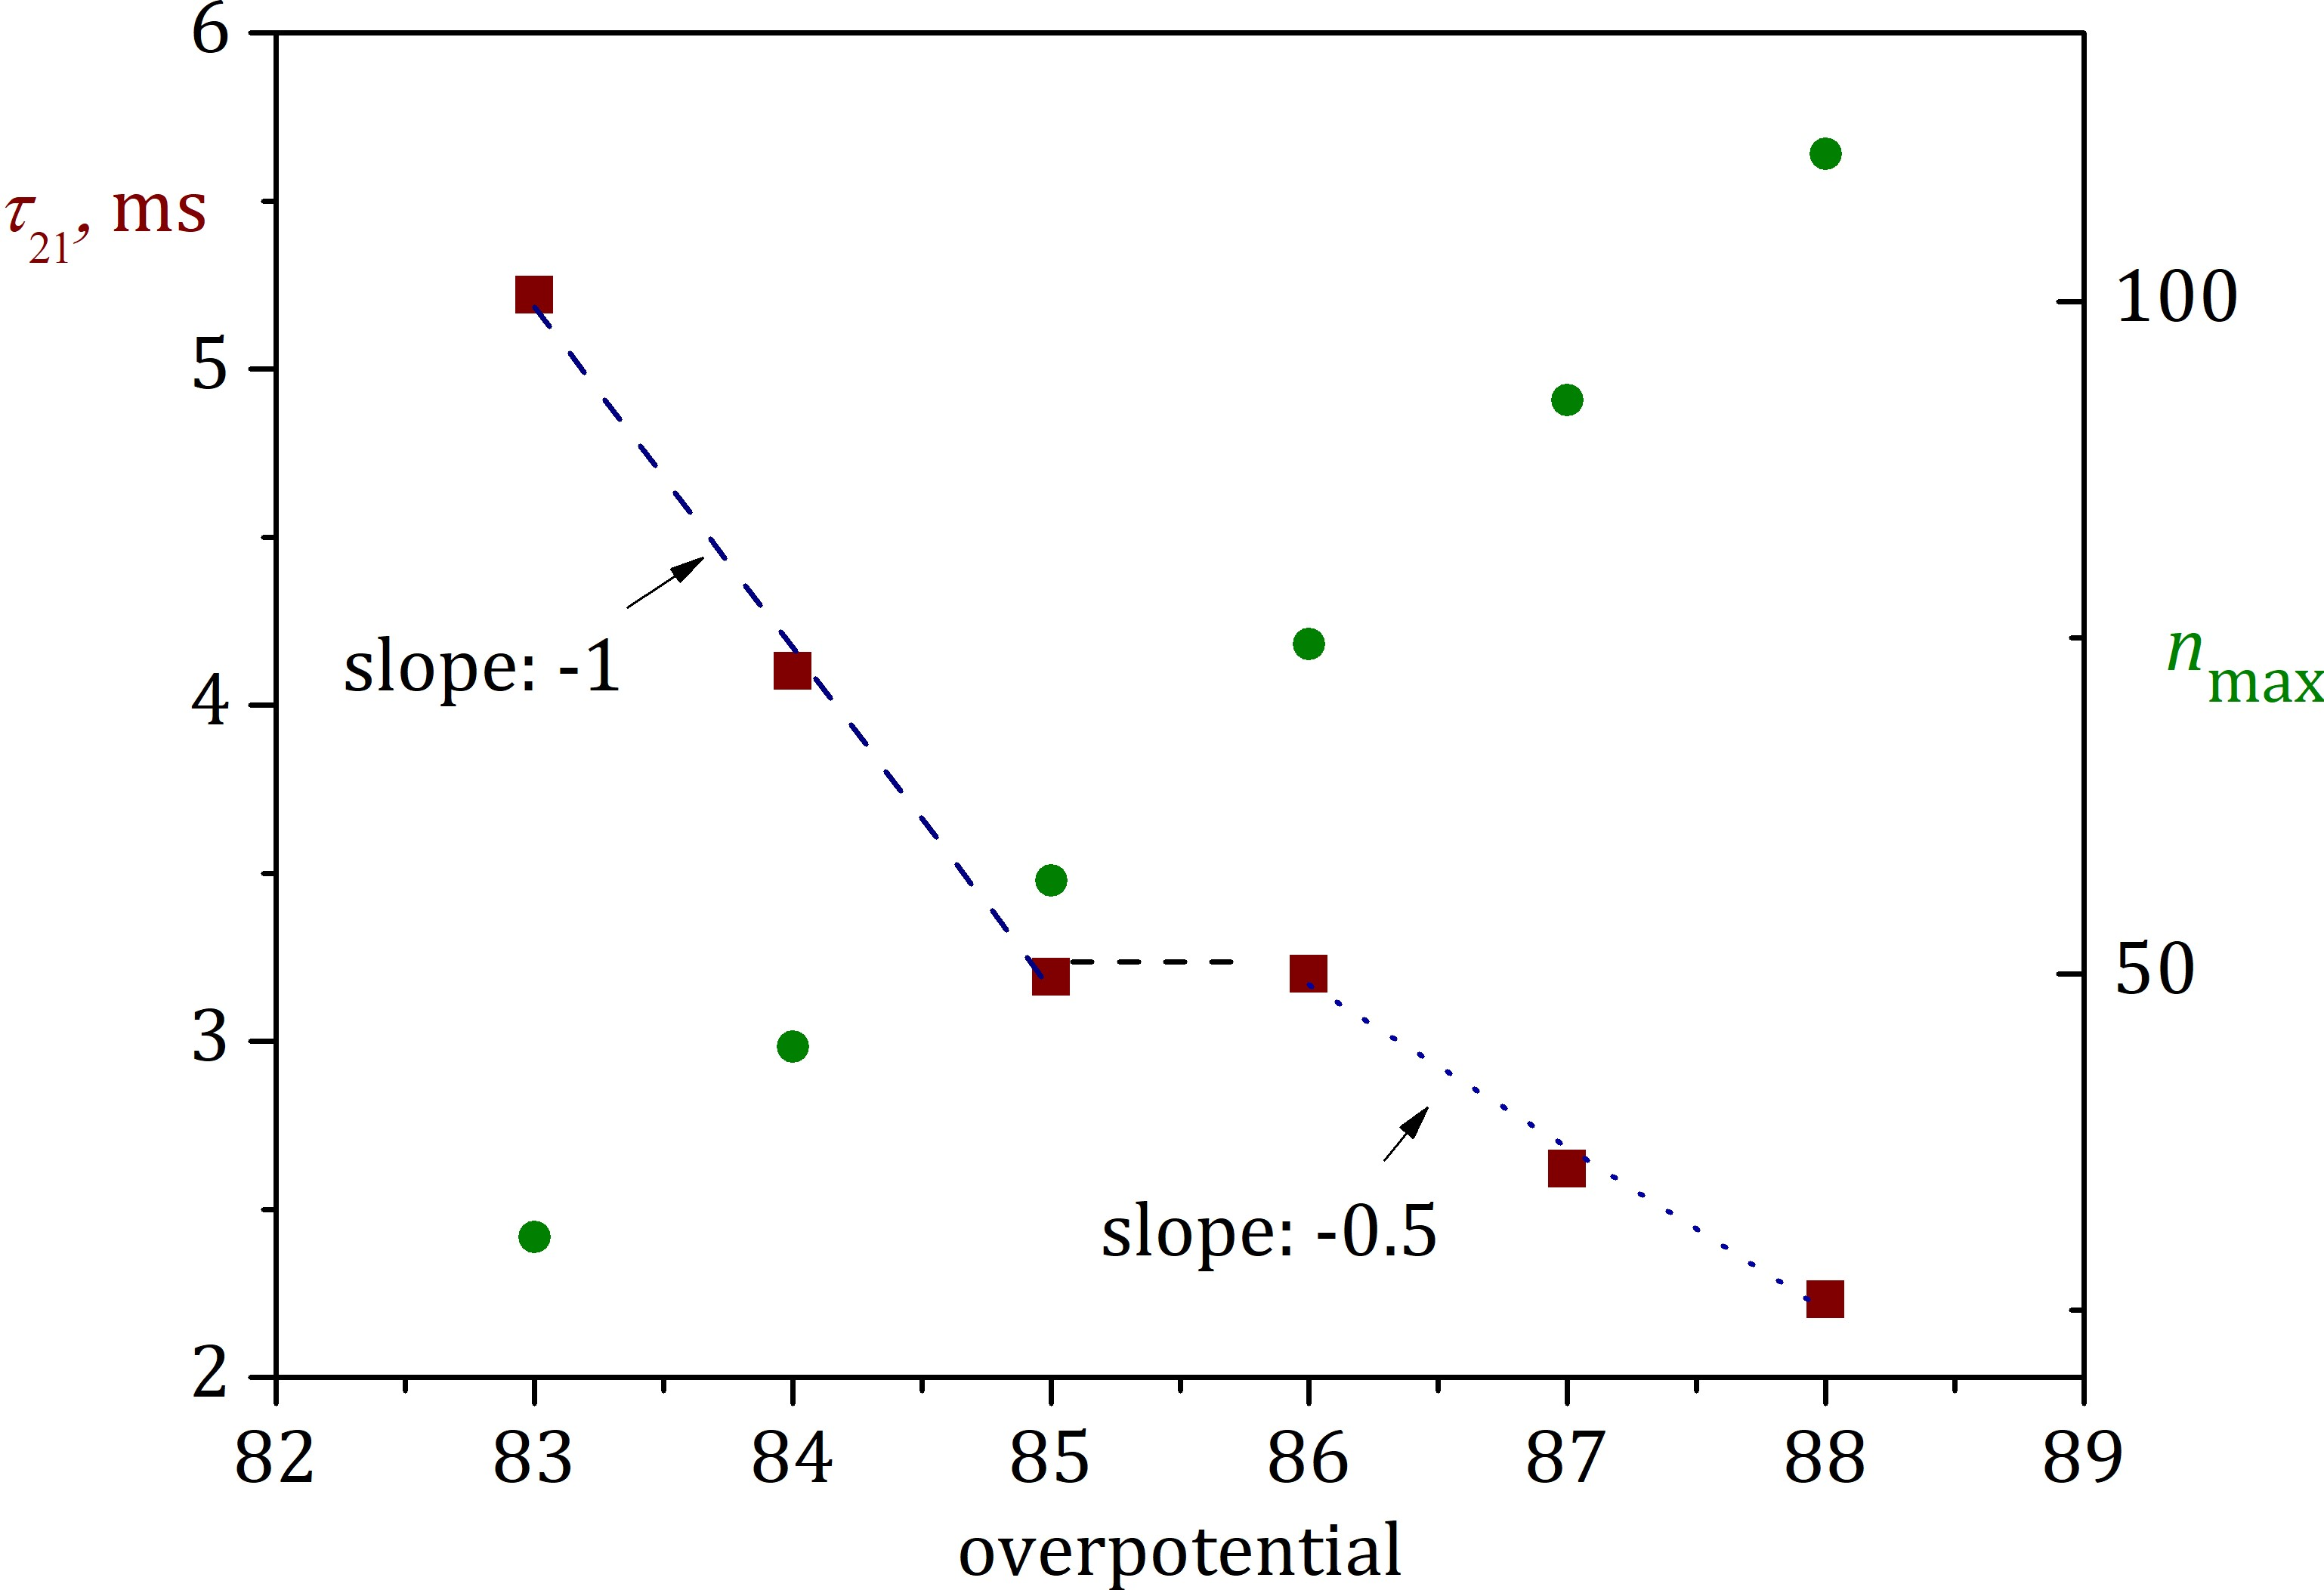
\includegraphics[width=0.48\textwidth]{ivan_markov_graphs/Fig5-alfa21_tau-overpotential.jpg}}
        \subfloat[Фиг. 6\label{subfig:alfa21_params_fig6}]{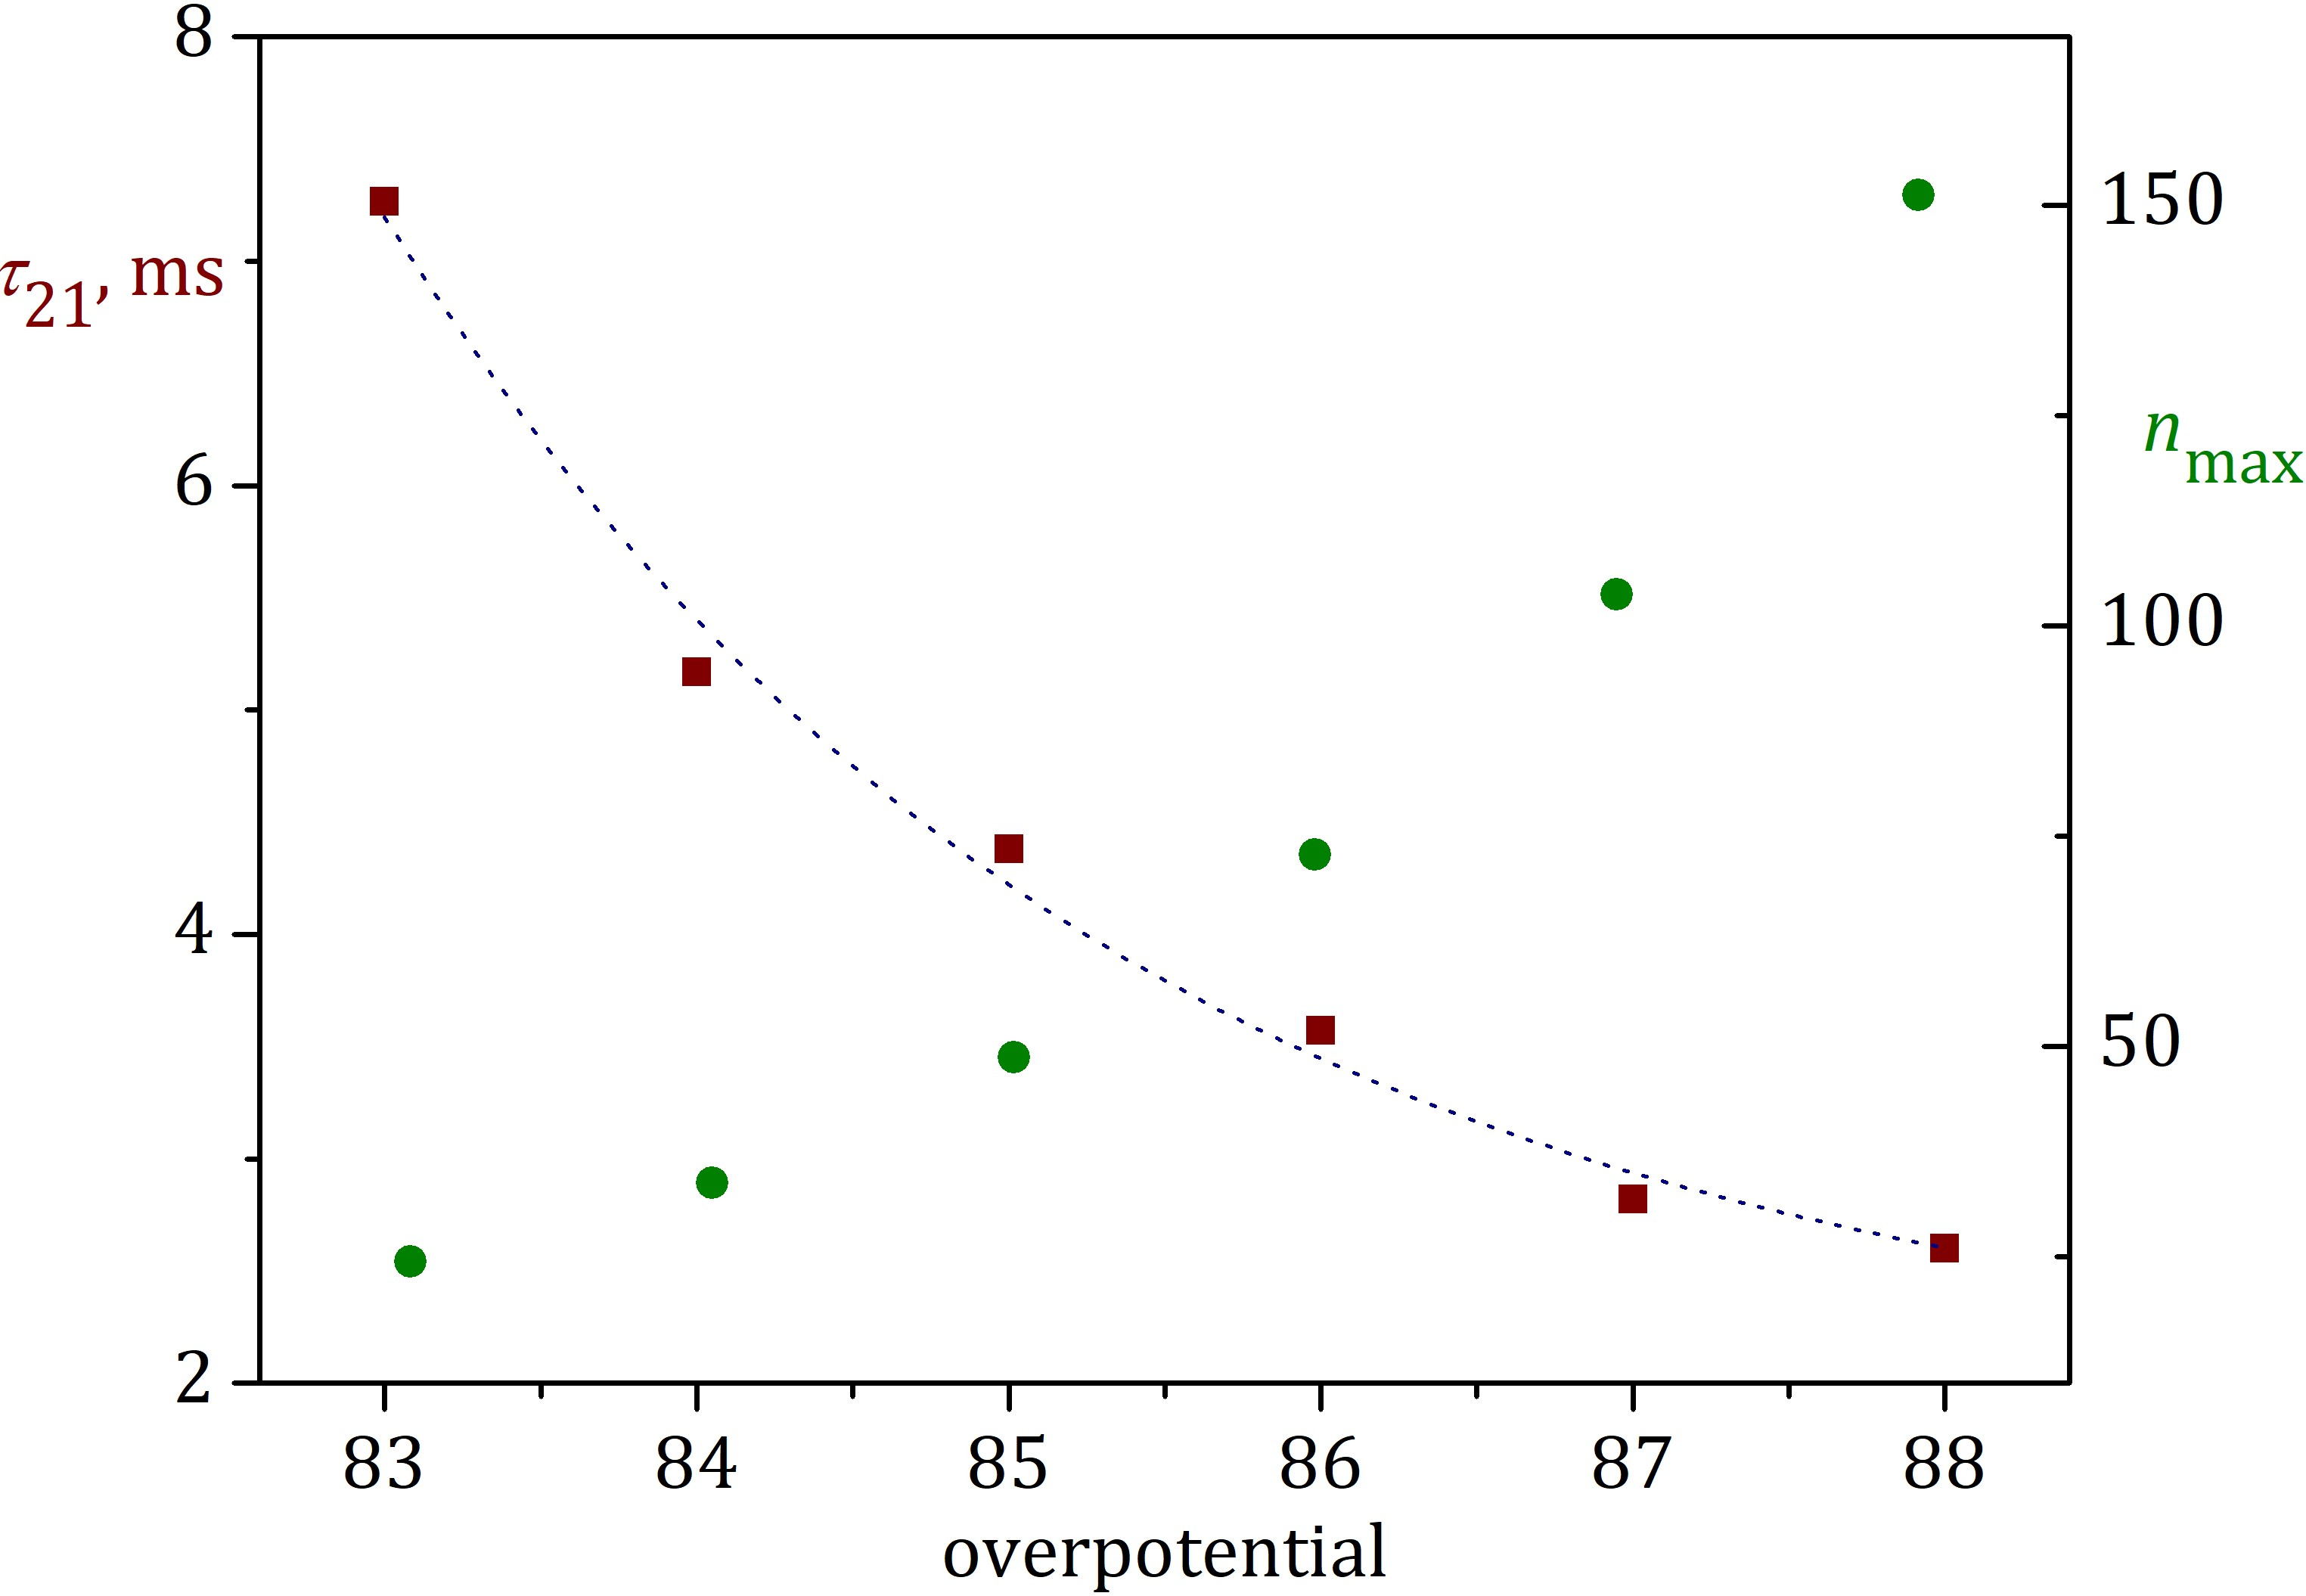
\includegraphics[width=0.48\textwidth]{ivan_markov_graphs/Fig6-alfa21_tau-overpotential.jpg}}  
    \caption[Зависимост на параметрите на модела от свръхпотенциала]{Зависимост на $N_{max}$ (\tikz\draw[darkgreen,fill=darkgreen] (0,0) circle (.5ex);) и $\tau_{21}$ (\tikz\draw[wine,fill=wine] (0,0) rectangle (1ex, 1ex);) от свръхпотенцила (пресищането) за $\alpha_{21}$}
    \label{fig:alfa21_ivan_markov_tau_nmax_overpot}
\end{figure}

\autoref{fig:alfa21_ivan_markov_tau_nmax_overpot} представлява връщането от безразмерна универсална крива - загуба на информация с цел потвърждаване на общия механизъм при различните експериментални условия. 

Изследването на зависимостта на скалите, с които е обезразмерен модела и как те зависят от свръхпотенциала (експерименталните условия) разкрива особености в поведението на системата.  На \autoref{subfig:alfa21_params_fig5} между $85~mV$ и $86~mV$ се наблюдава ясен сигнал за промяна на режима - наклонът на зависимостта $\tau_{21} (V)$ на практика намалява наполовина със скок. \autoref{subfig:alfa21_params_fig6} показва тъкмо обратното - гладко намаляване на характеристичното време $\tau_{21}$ с пресищането. В първия случай данните добре се описват от по части линейна зависимост, докато във втория - от квадратична.  Това поведение на $\tau_{21}$ във \autoref{fig:alfa21_ivan_markov_tau_nmax_overpot} може да бъде сравнено със спинодалния разпад в модела на Ван дер Ваалс за реалния газ (\textit{cusp catastrophy}).

При максималния брой зародиши подобна ,,катастрофа`` не се наблюдава в двата експеримента - и в двата случая имаме нарастване, което може да бъде описано с една гладка крива. На \autoref{subfig:alfa21_params_fig5} нарастването на максималния брой зародиши в системата $N_{max}$ е по-скоро линейно, докато \autoref{subfig:alfa21_params_fig6} е квадратично.

\subsubsection{Числени стойности на параметрите}
\autoref{tabl:fig5_table_data} и \autoref{tabl:fig6_table_data} показват, че на практика за всеки от моделите и наборите данни $R^2 \approx 0.99$, т.е. по този критерий (остатъчна дисперсия) те трудно могат да бъдат разделени. Максималният брой зародиши $N_{max}$ и времевите скали $\tau$ също са близки за всяка от колоните на таблиците (трудно можем да различим експериментално $N_{max} = 72, 74.5, 73$ например). Определящ тогава ще е изцяло броят параметри и физичният смисъл, който стои зад тях. 

При JMAKn не можем да дадем физическо обяснение за получените оптимални стойности за $n$, a фиксирането на $n = 2$ води до значително влошаване на $R^2$. Аналогично, при модела на Ричардс стойностите за $q$ не предполагат нито класически логистичен растеж, нито по модела на Гомперц. Фиксирането на този параметър също значително влошава $R^2$, като и физическото обяснение на параметрите е още по-трудно от това за JMAKn.

Изборът на конкретно кривата $\alpha_{21}$ \textit{a priori} предполага дифузионно контролиран квази-двумерен растеж, каквито и са заложените в експеримента условия. Параметрите $N_{max}$ и $\tau_{21}$ са напълно ясни в своя смисъл. Нещо повече - те представляват скалите за брой зародиши $N$ и време $t$, което позволява да получим универсалното поведение показано на \autoref{fig:alfa21_ivan_markov_master_curve}. 

За JMAKn и Ричардс параметрите не очертават ясна зависимост от свръхпотенциала. Експонентите $n$ и $q$ съответно и в двата случая намаляват и се насищат при високи потенциали. При, $\alpha_{21}$ както беше показано в предния параграф, се наблюдава интересна зависимост на времевата скала от експерименталните условия, което може да бъде основа на бъдещи изследвания.
\begin{table}[hb]
\centering
\caption{Данни за параметрите от фиг. 5 получени от моделите в йерархията. Скалата за Ричардс не е получена директно от фитването на данните. Параметрите $t_i$ и $t_k$ не са показани, тъй като не са използвани в дискусията на резултатите.}
\label{tabl:fig5_table_data}
\resizebox{\textwidth}{!}{%
\begin{tabular}{cccccccccccc} 
\toprule
\multirow{2}{*}{overvoltage, mV} & \multicolumn{3}{c}{$\alpha_{21}$}                                                           & \multicolumn{4}{c}{JMAKn}                                                                                                & \multicolumn{4}{c}{Richards}                                                                                           \\
                                 & \multicolumn{1}{l}{$N_{max}$} & \multicolumn{1}{l}{$\tau_{21}$} & \multicolumn{1}{l}{$R^2$} & \multicolumn{1}{l}{$N_{max}$} & \multicolumn{1}{l}{$\tau_{JMAKn}$} & \multicolumn{1}{l}{$n$} & \multicolumn{1}{l}{$R^2$} & \multicolumn{1}{l}{$N_{max}$} & \multicolumn{1}{l}{$\tau_{21}$} & \multicolumn{1}{l}{$q$} & \multicolumn{1}{l}{$R^2$}  \\ 
\hline
83                               & 30.43                         & 5.22                            & 0.9974                    & 29.9                          & 5.6                                & 1.89                    & 0.9977                    & 30.29                         & 5.20                            & 0.83                    & 0.9967                     \\
84                               & 44.61                         & 4.11                            & 0.9937                    & 45.78                         & 4.75                               & 1.39                    & 0.9986                    & 46.28                         & 3.93                            & 0.53                    & 0.9981                     \\
85                               & 56.94                         & 3.19                            & 0.9986                    & 56.86                         & 3.51                               & 1.67                    & 0.998                     & 57.36                         & 3.28                            & 0.64                    & 0.9984                     \\
86                               & 74.51                         & 3.20                            & 0.9976                    & 75.06                         & 3.61                               & 1.58                    & 0.9992                    & 75.60                         & 3.09                            & 0.79                    & 0.9988                     \\
87                               & 92.7                          & 2.62                            & 0.9988                    & 92.37                         & 2.89                               & 1.70                    & 0.9995                    & 93.17                         & 2.52                            & 0.96                    & 0.9989                     \\
88                               & 111.01                        & 2.23                            & 0.9974                    & 109.19                        & 2.40                               & 1.86                    & 0.999                     & 109.57                        & 2.09                            & 1.35                    & 0.9983                     \\
\bottomrule
\end{tabular}
}
\end{table}

\begin{table}[hb]
\centering
\caption{Данни за параметрите от фиг. 6 получени от моделите в йерархията. Аналогично на Фиг.5 скалата за Ричардс е получена индиректно и параметрите $t_i$ и $t_k$ не са показани.}
\label{tabl:fig6_table_data}
\resizebox{\textwidth}{!}{%
\begin{tabular}{cccccccccccc} 
\toprule
\multirow{2}{*}{overvoltage, mV} & \multicolumn{3}{c}{$\alpha_{21}$} & \multicolumn{4}{c}{JMAKn}                  & \multicolumn{4}{c}{Richards}            \\
                                  & $N_{max}$ & $\tau_{21}$ & $R^2$   & $N_{max}$ & $\tau_{JMAKn}$ & $n$  & $R^2$  & $N_{max}$ & $\tau_{R}$ & $q$  & $R^2$   \\ 
\hline
83                                & 24.41     & 7.27        & 0.9966  & 23.92     & 7.79           & 1.91 & 0.9978 & 24.12     & 6.95       & 1.18 & 0.9963  \\
84                                & 33.84     & 5.17        & 0.9977  & 33.68     & 5.69           & 1.72 & 0.9978 & 33.93     & 4.98       & 0.93 & 0.9971  \\
85                                & 48.69     & 4.38        & 0.9969  & 48.97     & 4.92           & 1.55 & 0.9985 & 48.19     & 4.62       & 0.43 & 0.9987  \\
86                                & 72.78     & 3.57        & 0.9890  & 74.50     & 4.13           & 1.38 & 0.9967 & 73.07     & 3.36       & 0.51 & 0.9948  \\
87                                & 103.77    & 2.82        & 0.9923  & 106.51    & 3.30           & 1.38 & 0.9993 & 103.81    & 2.68       & 0.54 & 0.9990  \\
88                                & 151.22    & 2.60        & 0.9891  & 156.27    & 3.03           & 1.35 & 0.9971 & 151.30    & 2.43       & 0.52 & 0.9958  \\
\bottomrule
\end{tabular}
}
\end{table}